\documentclass{pracalicmgr}
\usepackage[utf8]{inputenc}
\usepackage{graphicx}
\usepackage{textcomp}
\usepackage{titlesec}
\usepackage[T1]{fontenc}
\usepackage{float}
\usepackage[english]{babel}
\usepackage{gensymb}
\usepackage{enumitem}
\usepackage{chngcntr}
\usepackage{epstopdf}
\usepackage{color}
\usepackage{indentfirst}
\usepackage{mathtools}
\usepackage{lmodern}
\usepackage{amsfonts}
\usepackage{hyperref}
\usepackage{xurl}
\usepackage{braket}
\usepackage{amsmath}
\usepackage{longtable}
%\setcounter{secnumdepth}{4}
\usepackage{wrapfig}

%\linespread{2}
\raggedbottom
%\counterwithin{figure}{section}

\author{Wojciech Noskowiak}

\nralbumu{417909}

\title{Calculations of electric dipole moments in two-electron diatomic molecules}

\tytulang{Obliczenia elektrycznych momentów dipolowych dla dwuelektronowych dwuatomowych cząsteczek}

\kierunek{Physics}

%\specjalnosc{Metody jądrowe w fizyce ciała stałego}

\opiekun{\\prof. dr hab. Krzysztof Pachucki\\Chair of quantum optics and atomic physics\\ Institute of Theoretical Physics\\\vspace{0.3cm plus 1.5fill}\\mgr Michał Siłkowski\\Chair of quantum optics and atomic physics\\ Institute of Theoretical Physics\\}

%\dziedzina{13.200}
\dziedzina{13.2 Fizyka}

\date{September 2022}

\keywords{High-precision calculations, dipole moment, two-electron diatomic molecules, helium hydride ion, Kołos-Wolniewicz, variational method, electronic structure}

\overfullrule=1pt
\begin{document}
\maketitle
\let\cleardoublepage\clearpage

\begin{abstract}
    An efficient approach to high-precision calculations of expectation values of electronic operators in two-electron diatomic molecules is outlined and explored. A detailed description of the method and its usefulness is provided and illustrated with numerical calculations of the permanent dipole moment and energy of the HeH\textsuperscript{+} molecule in its ground state. A comparison of obtained results against values present in the literature is provided and discussed.
\end{abstract}

\tableofcontents

\newpage

\chapter*{Introduction}
\label{sec:intro}
\addcontentsline{toc}{chapter}{\nameref{sec:intro}}

Diatomic two-electron molecules have historically been a common subject of research in quantum electrodynamics.

The simple structure of those systems allows one to perform calculations with very high precision, which in turn makes possible the verification of the quantum electrodynamics theory. 

This work explores a computationally efficient method of performing numerical calculations for diatomic two-electron particles with arbitrary precision. A program implementing such a method is also described. 

This thesis also provides an example calculation made with said software, specifically it attempts to calculate the ground state energy and the permanent dipole moment of the HeH\textsuperscript{+} molecule. 

The precise values of the permanent dipole moment for this molecule weren't previously calculated. It also has a significant role in astrophysics and chemistry. It is the simplest polar hetero-nuclear molecule, and was also abundantly present in the early universe. \cite{chem} \cite{astro}
 

\chapter{Kołos-Wolniewicz basis and the \texorpdfstring{$f$}{TEXT} function formalism}
\label{rob}

\section{Description of the system}

\begin{figure}[H]
    \center
    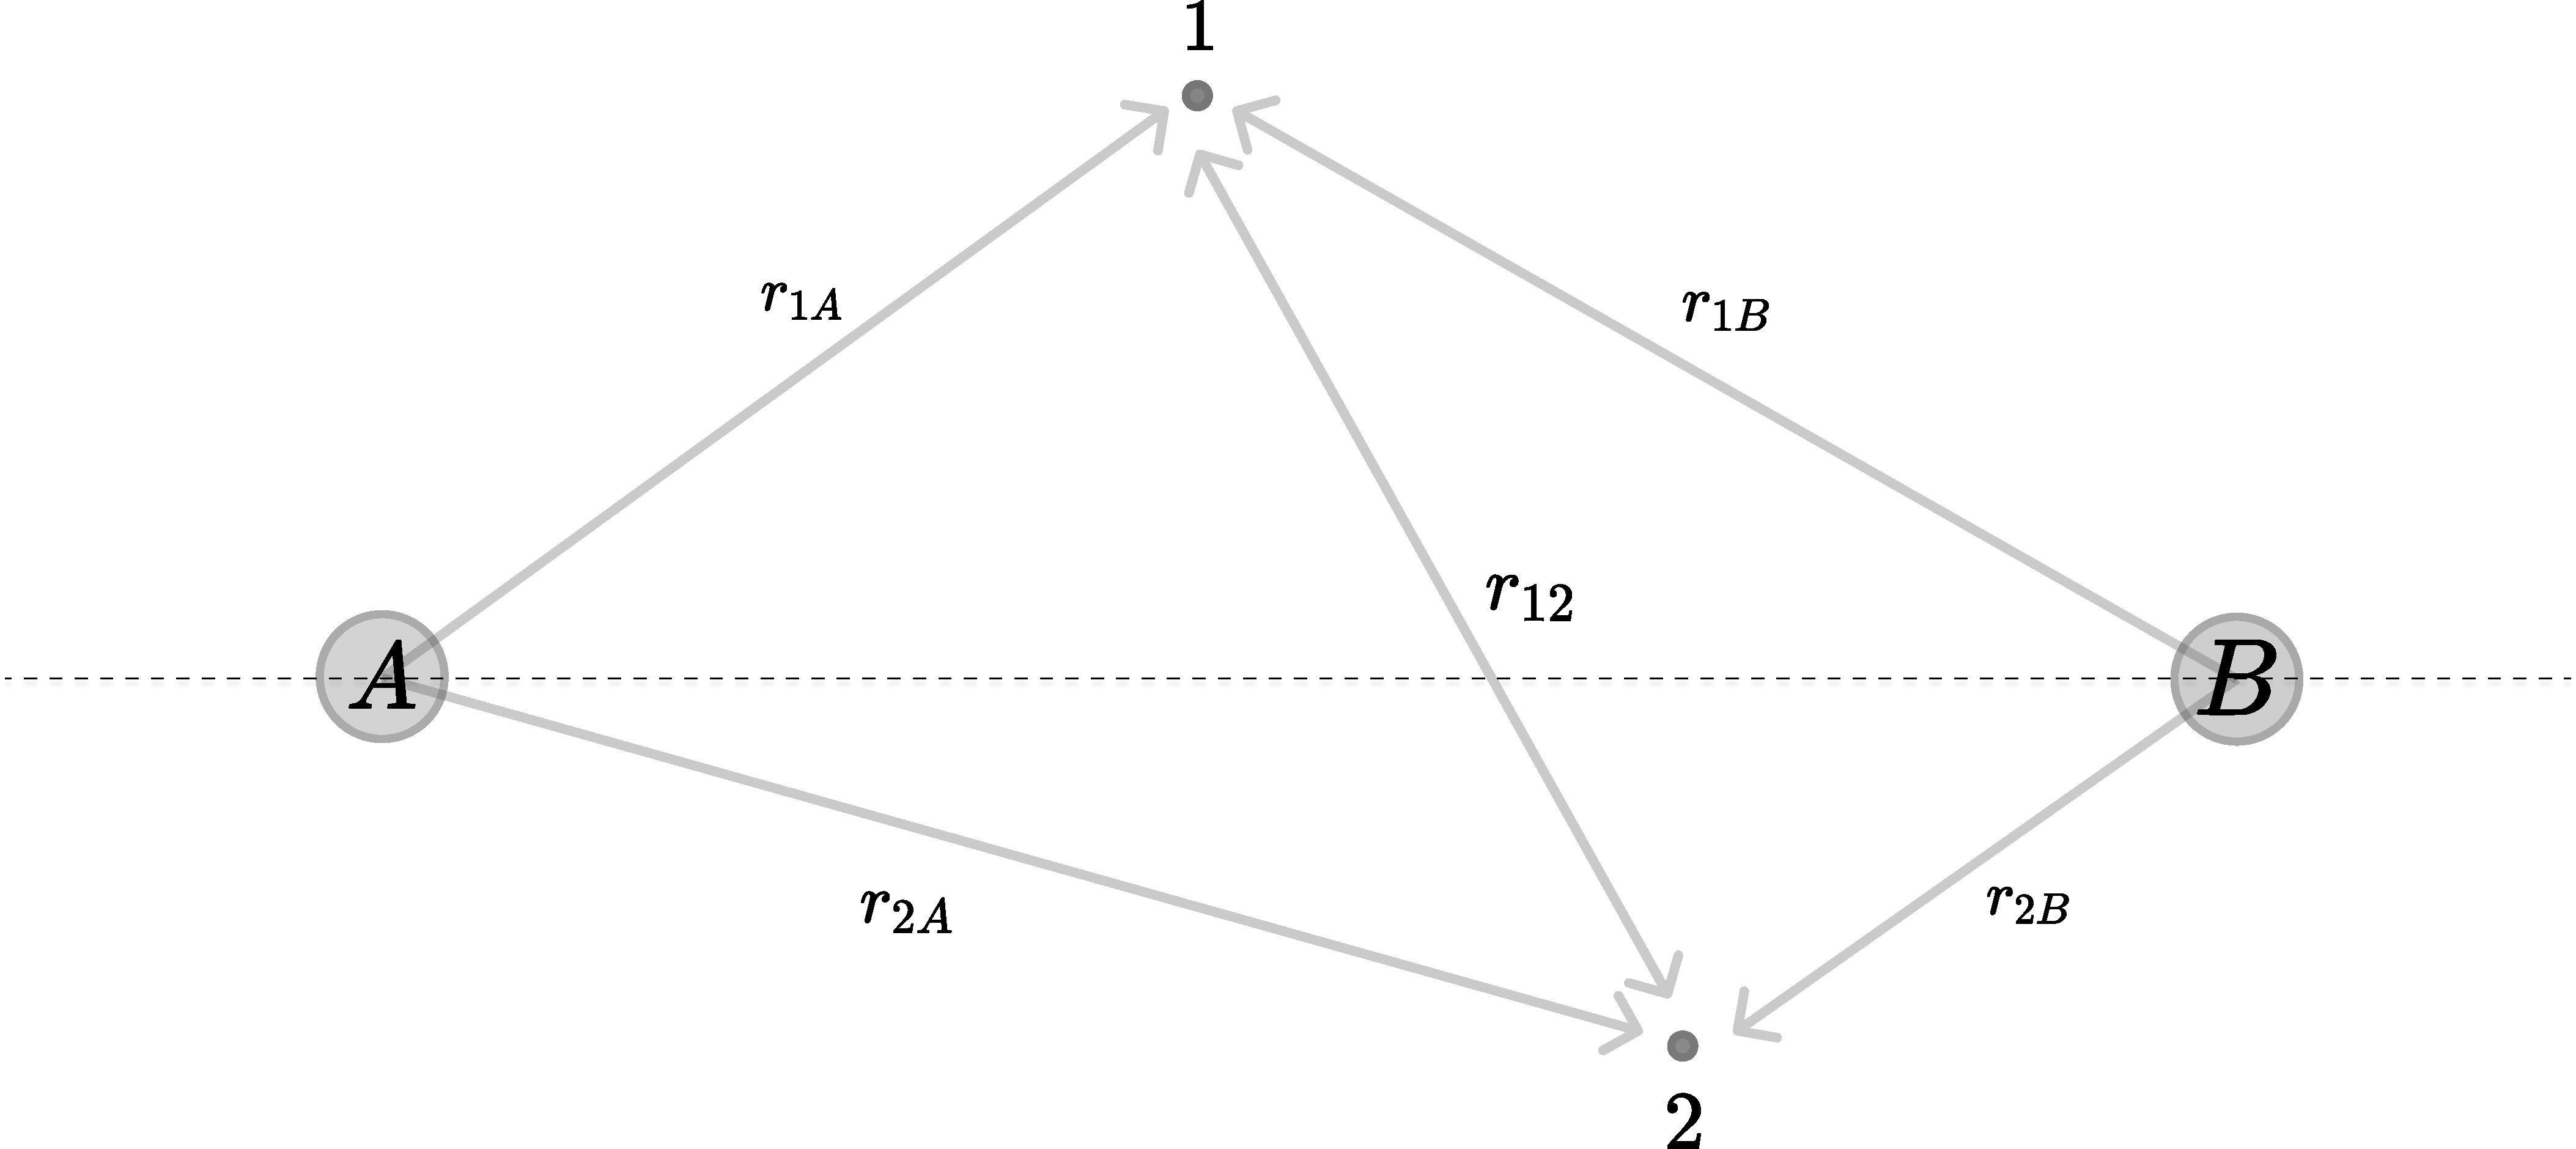
\includegraphics[width=0.6\textwidth]{system.pdf}
    \caption{Visual representation of the system}
    \label{system}
\end{figure}

The two electron diatomic particle described in the title will be represented by a system comprised of two electrons and two nuclei.

In the latter used convention aliases $1$ and $2$ will be assigned to each of the electrons. Similarly, aliases $A$ and $B$ will be used to describe the nuclei. Henceforth, the distance between two elements of the system will be denoted as $r$ with the aliases of its two defining elements in its subscript (e.g. $r_{12}$ represents the distance between the electrons). Mass of each of the nuclei will be represented by $M$ with the alias of the nuclei in its subscript

\section{Kołos-Wolniewicz basis}

\subsection{Description of the basis}

The calculations will be performed using the method first described in \cite{metoda} that builds upon the way Kołos and Wolniewicz \cite{Kolos1} \cite{Kolos2} performed calculations of the ground state energies of the $H_2$ molecule. This method allows for an efficient and precise numerical calculation of the ground state energy of diatomic two electron molecules as well as the expected values of a plethora of operators.

The method uses the Kołos-Wolniewicz basis, which is  defined as a family of functions described by the equation
\begin{multline}
    \psi_{n_0 n_1 n_2 n_3 n_4} \left( r_{1A}, r_{1B}, r_{2A}, r_{2B}, r_{12} \right) = e^{-y\left(r_{1A}-r_{1B}\right)-x\left(r_{2A}-r_{2B}\right)-u\left(r_{1A}+r_{1B}\right)-w\left(r_{2A}+r_{2B}\right)}\\
    r_{12}^{n_0}{\left(r_{1A}-r_{1B}\right)}^{n_1}{\left(r_{2A}-r_{2B}\right)}^{n_2}{\left(r_{1A}+r_{1B}\right)}^{n_3}{\left(r_{2A}+r_{2B}\right)}^{n_4}
    \label{KWdef}
\end{multline}

For all natural values of the $n$. Here nonlinear parameters $y$, $x$, $u$ and $w$ characterize the specific basis and are the same for all of it's comprising functions.
The dependence of the basis functions on the distance between the electrons (represented by $R_{12}$) makes the basis explicitly correlated, allowing it to accurately describe the two-electron system 

It should be noted at this point that the above described basis is not orthogonal, but in light of its  mathematical properties that will be described later this does not diminish its practicality.

\subsection{Interpretation of the linear combinations of interelectronic coordinates}

\begin{figure}[H]
    \center
    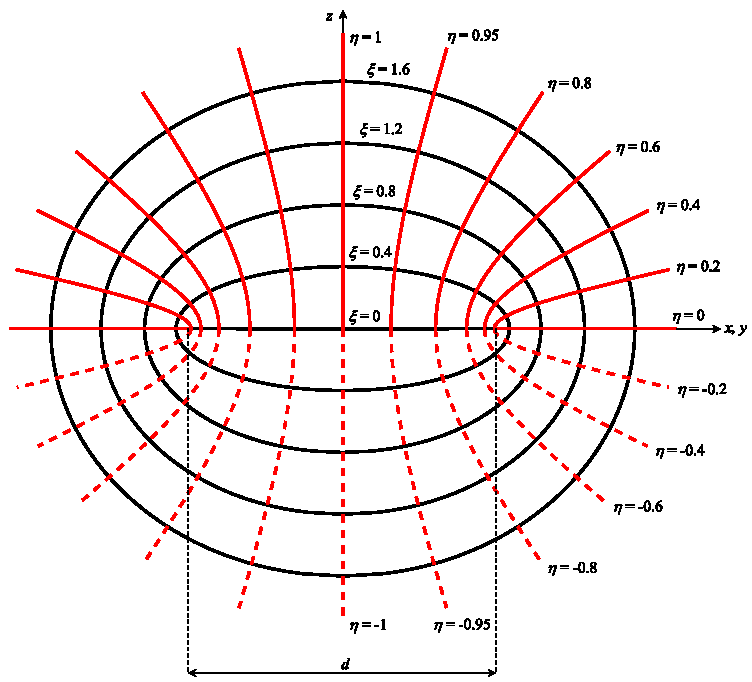
\includegraphics[width=0.70\textwidth]{oblate.pdf}
    \caption{Representation of the elliptic coordinate system, source: \cite{EllipticRys} }
    \label{eliptical}
\end{figure}

It can be observed that the functions in question can be trivially restated as a function dependent on variables $\left(r_{1A}-r_{1B}\right)$, $\left(r_{2A}-r_{2B}\right)$, $\left(r_{1A}+r_{1B}\right)$ and $\left(r_{2A}+r_{2B}\right)$. In the case of a diatomic system these variables can be interpreted respectively as $\zeta_1$, $\zeta_2$, $\eta_1$ and $\eta_2$ in the elliptic coordinate system\cite{eliptic_article} with its focal points placed at the nuclei. Such an interpretation allows one to intuitionally understand why the Kołos-Wolniewicz basis provides a set of functions that properly represents the problem at hand.

\section{Master integral and the \texorpdfstring{$f$}{TEXT} functions}

The usefulness of the chosen method arises from its use of the relation between the family of functions derived from the so-called master integral and the elements of the aforementioned Kołos-Wolniewicz basis.

The master integral is given by the equation

\begin{equation}
    f\left(r\right) = \int{\frac{d^3 r_1}{4 \pi}}\int{\frac{d^3 r_2}{4 \pi}}\frac{e^{-wr_{12}-y\left(r_{1A}-r_{1B}\right)-x\left(r_{2A}-r_{2B}\right)-u\left(r_{1A}+r_{1B}\right)-w\left(r_{2A}+r_{2B}\right)}}{r_{1A} r_{1B} r_{2A} r_{2B} r_{12}}
    \label{MasInt}
\end{equation}

and the family of function is described by

\begin{multline}
    f\left(r,n_0, n_1, n_2, n_3, n_4\right) = \frac{r}{n_0! n_1! n_2! n_3! n_4!} \int{\frac{d^3 r_1}{4 \pi}}\int{\frac{d^3 r_2}{4 \pi}}r_{12}^{n_0}{\left(r_{1A}-r_{1B}\right)}^{n_1}{\left(r_{2A}-r_{2B}\right)}^{n_2}\\
    {\left(r_{1A}+r_{1B}\right)}^{n_3}{\left(r_{2A}+r_{2B}\right)}^{n_4}\frac{e^{-wr_{12}-y\left(r_{1A}-r_{1B}\right)-x\left(r_{2A}-r_{2B}\right)-u\left(r_{1A}+r_{1B}\right)-w\left(r_{2A}+r_{2B}\right)}}{r_{1A} r_{1B} r_{2A} r_{2B} r_{12}}
    \label{f elem}
\end{multline}

For all natural values of $n$.

It should be noted at this point that the non-linear parameter $w$ is present in \ref{MasInt} and \ref{f elem} purely as a mathematical device that proves to be essential in the derivations of relationships defined further, and will later be assumed to have a value of $0$.

The $f$ function described above is essentially an integral of the corresponding function from the previously defined Kołos-Wolniewicz basis \ref{KWdef} $\psi_{n_0 n_1 n_2 n_3 n_4}$ divided by the factor ${r_{1A} r_{1B} r_{2A} r_{2B} r_{12}}$ and integrated over the entire space. Therefore, if a specific operator can be expressed as a polynomial comprised of the different $r$ values then every one of its matrix components can be represented as a linear combination of $f$ functions. For example the element of the overlap matrix is given by

\begin{multline}
    \bra{k_0,\cdots,k_4}\ket{l_0,\cdots,l_4} = \frac{1}{16}
    \left(
    f\left(1 + n_1,n_2,n_3,2 + n_4,2 + n_5\right)\right. -\\ 
    f\left(1 + n_1,n_2,2 + n_3,2 + n_4,n_5\right) - \\
    f\left(1 + n_1,2 + n_2,n_3,n_4,2 + n_5\right) + \\
    \left.f\left(1 + n_1,2 + n_2,2 + n_3,n_4,n_5\right)\right) \\
    \label{overlap}
\end{multline}

where $n_a = k_a + l_a$

Such representation of the matrix element of a specific operator will thereafter be referred to as $f$ function formalism

It should be noted at this point that in further calculation the elements of the overlap matrix will be assumed to be dimensionless. This should be taken into account when representing the operators in the $f$ function formalism, as the dimension of the $f$ function is dependent on the sum of the $n$ parameters\ref{f elem}

It can be observed that all $f$ functions are, in essence, the master integral \ref{MasInt} differentiated a specific number of times in regard to each of the nonlinear coefficients. Specifically

\begin{multline}
    f\left(r,n_0, n_1, n_2, n_3, n_4\right) = \\
    \frac{r}{n_0! n_1! n_2! n_3! n_4!} {\left.{\left(-\frac{\partial}{\partial w}\right)}^{n_0}\right|}_{w=0}{\left(-\frac{\partial}{\partial y}\right)}^{n_1} {\left(-\frac{\partial}{\partial x}\right)}^{n_2} {\left(-\frac{\partial}{\partial u}\right)}^{n_3}{\left(-\frac{\partial}{\partial w}\right)}^{n_4} f\left(r\right)
    \label{DeriDef}
\end{multline}

Therefore, knowing the value of the master integral \ref{MasInt} one can easily obtain any other $r$ function.

\section{Method of calculating the \texorpdfstring{$f$}{TEXT} functions}

\begin{figure}[H]
    \center
    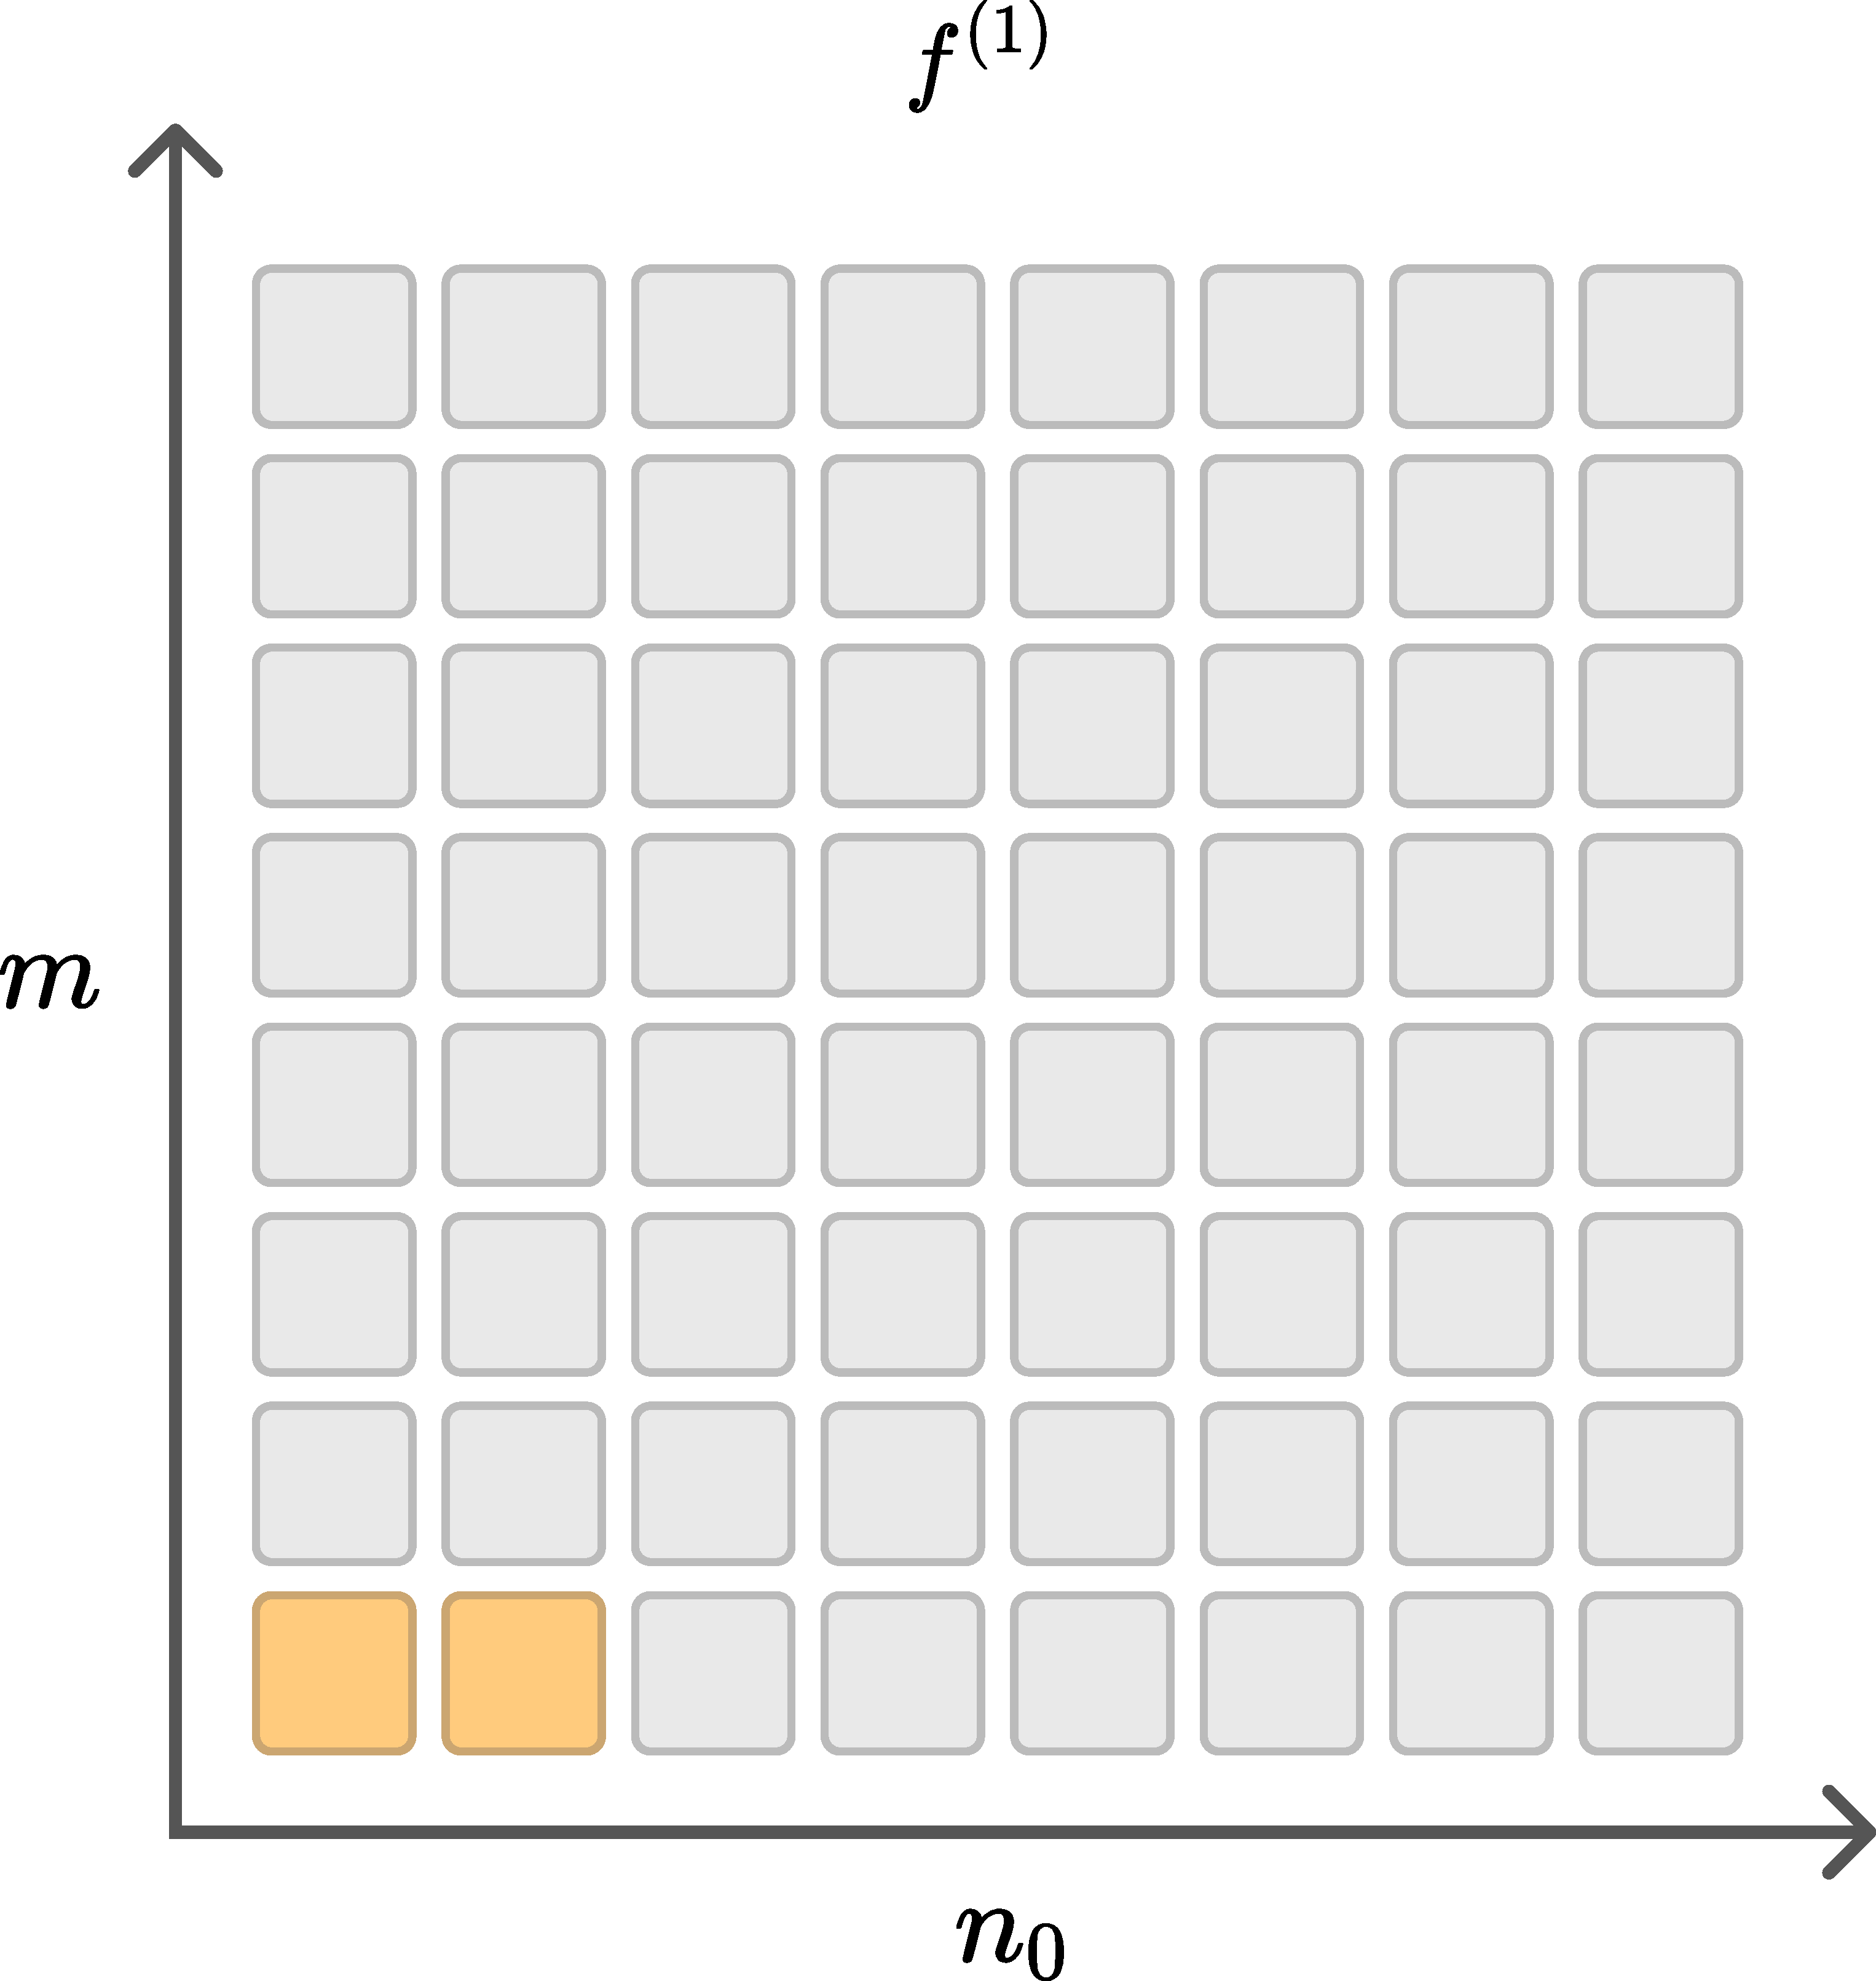
\includegraphics[width=0.30\textwidth]{uno.pdf}
    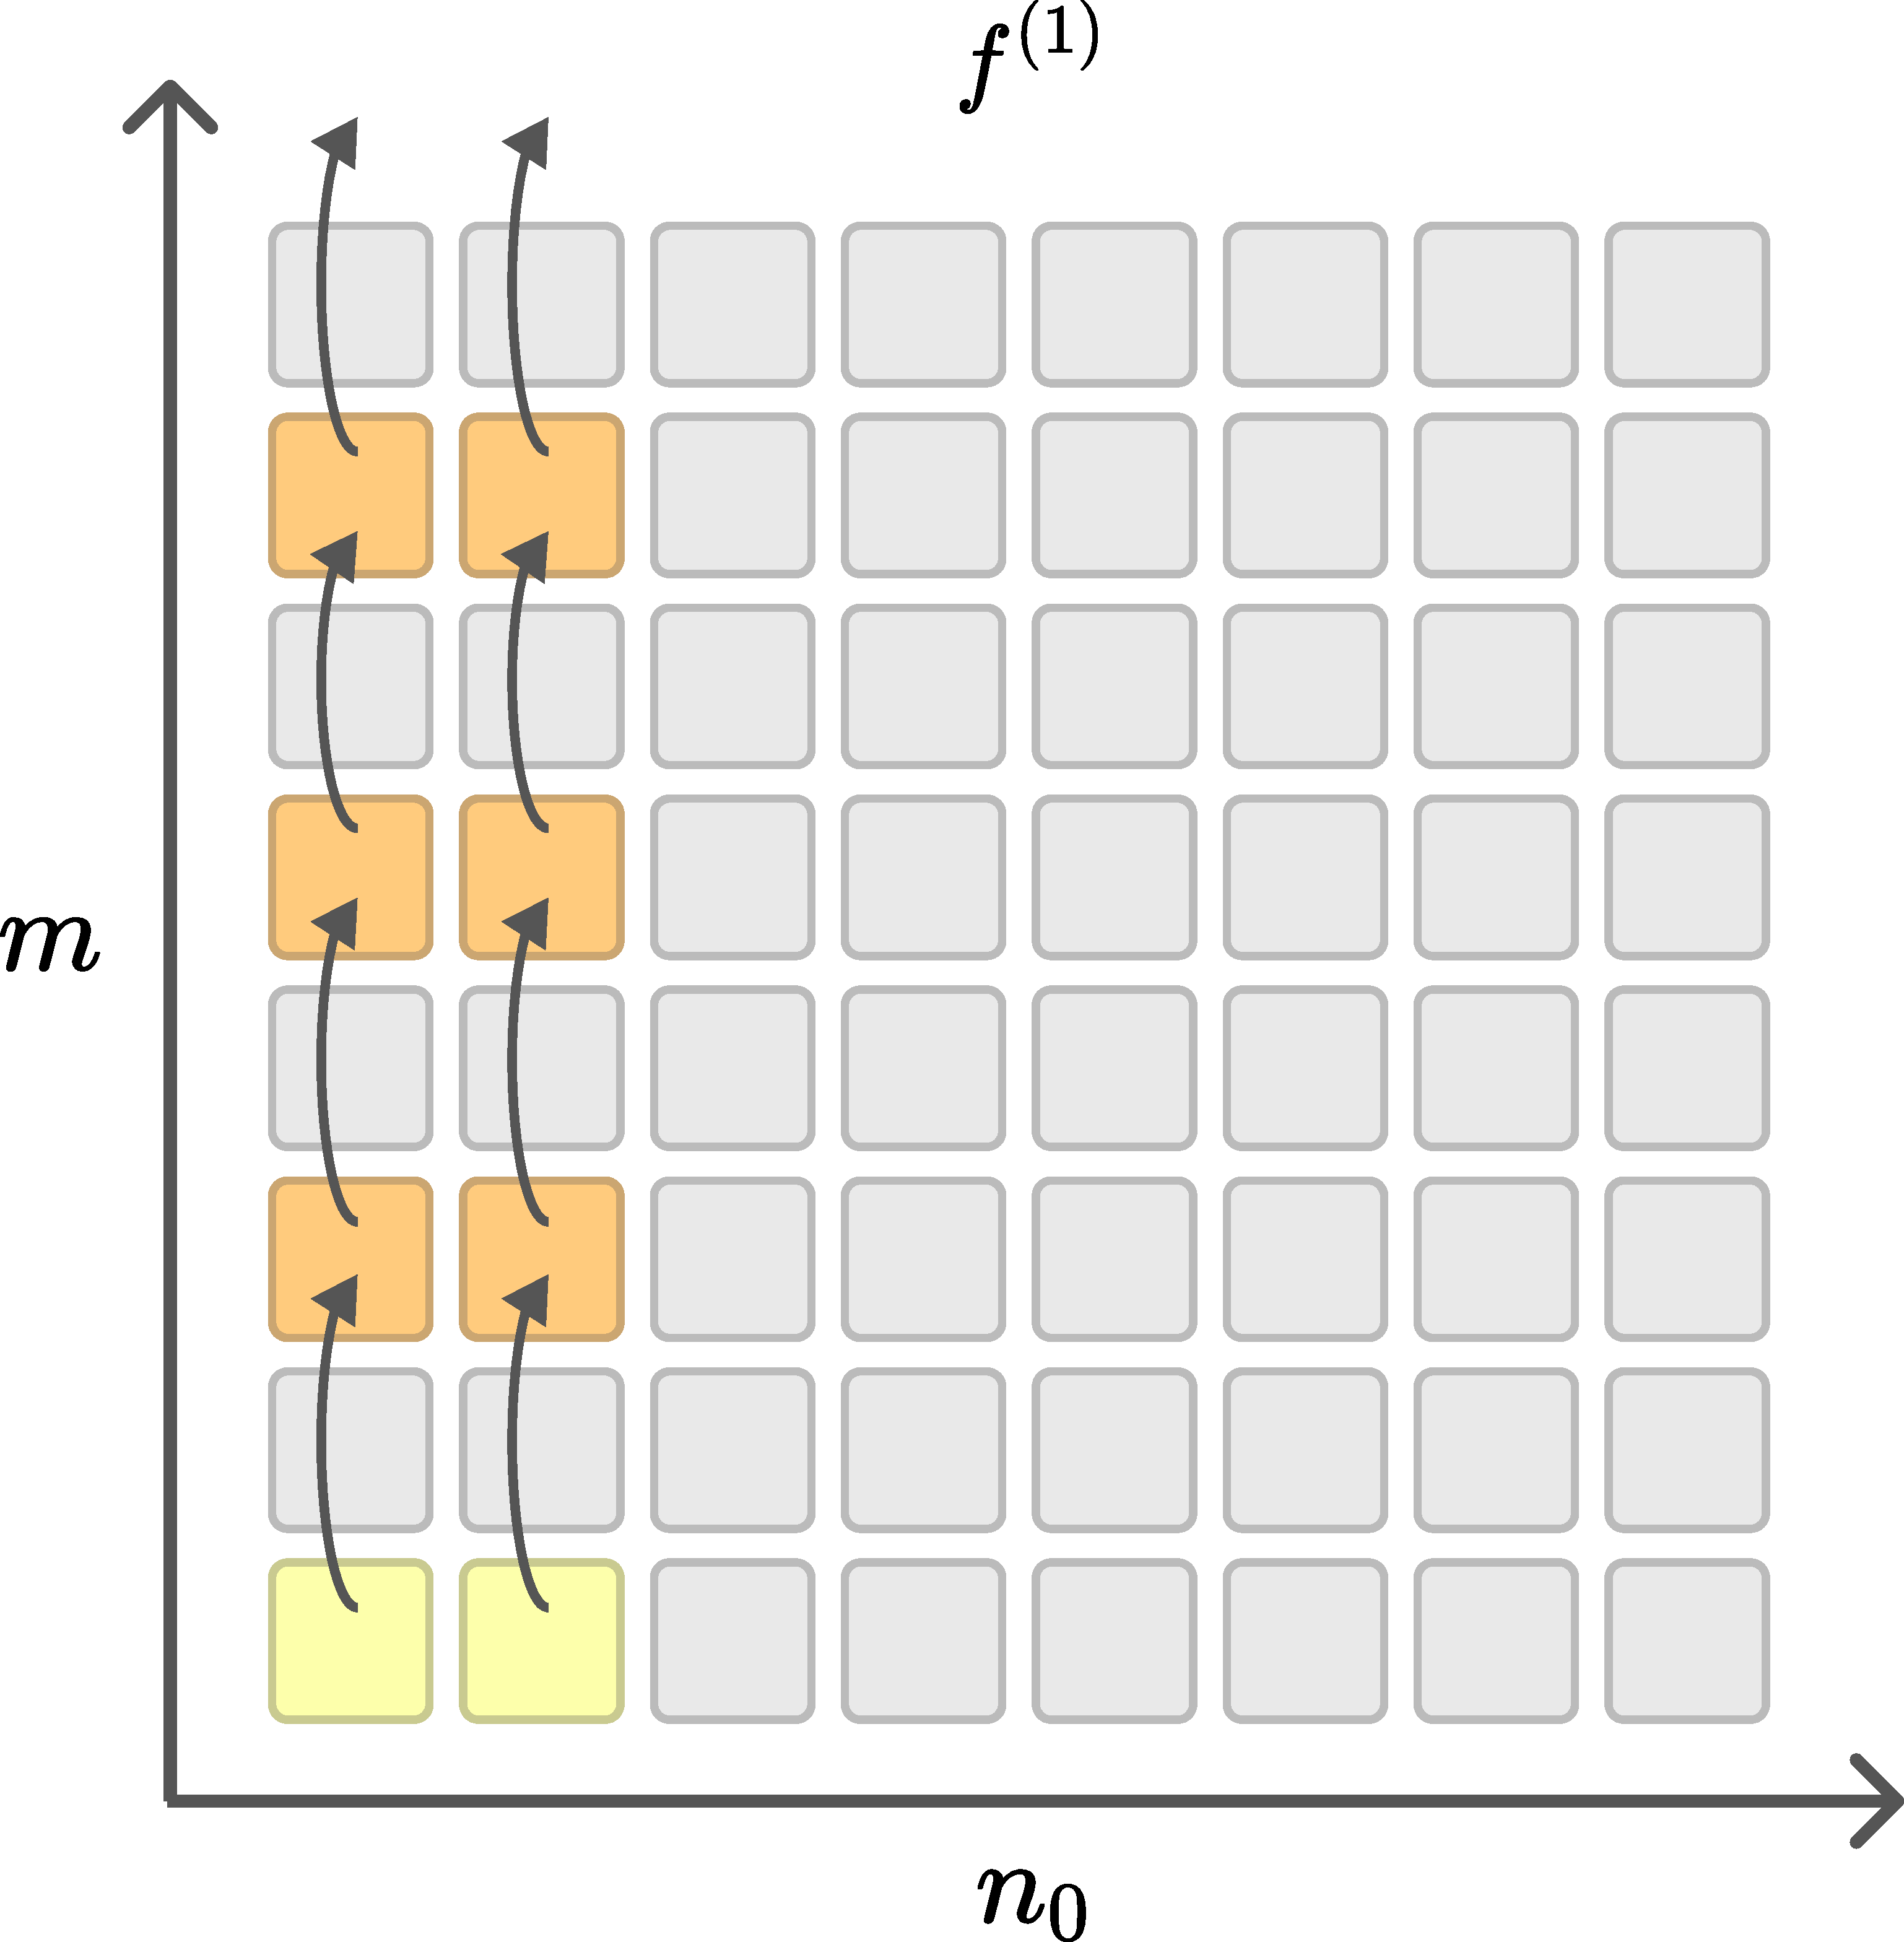
\includegraphics[width=0.30\textwidth]{dos.pdf}
    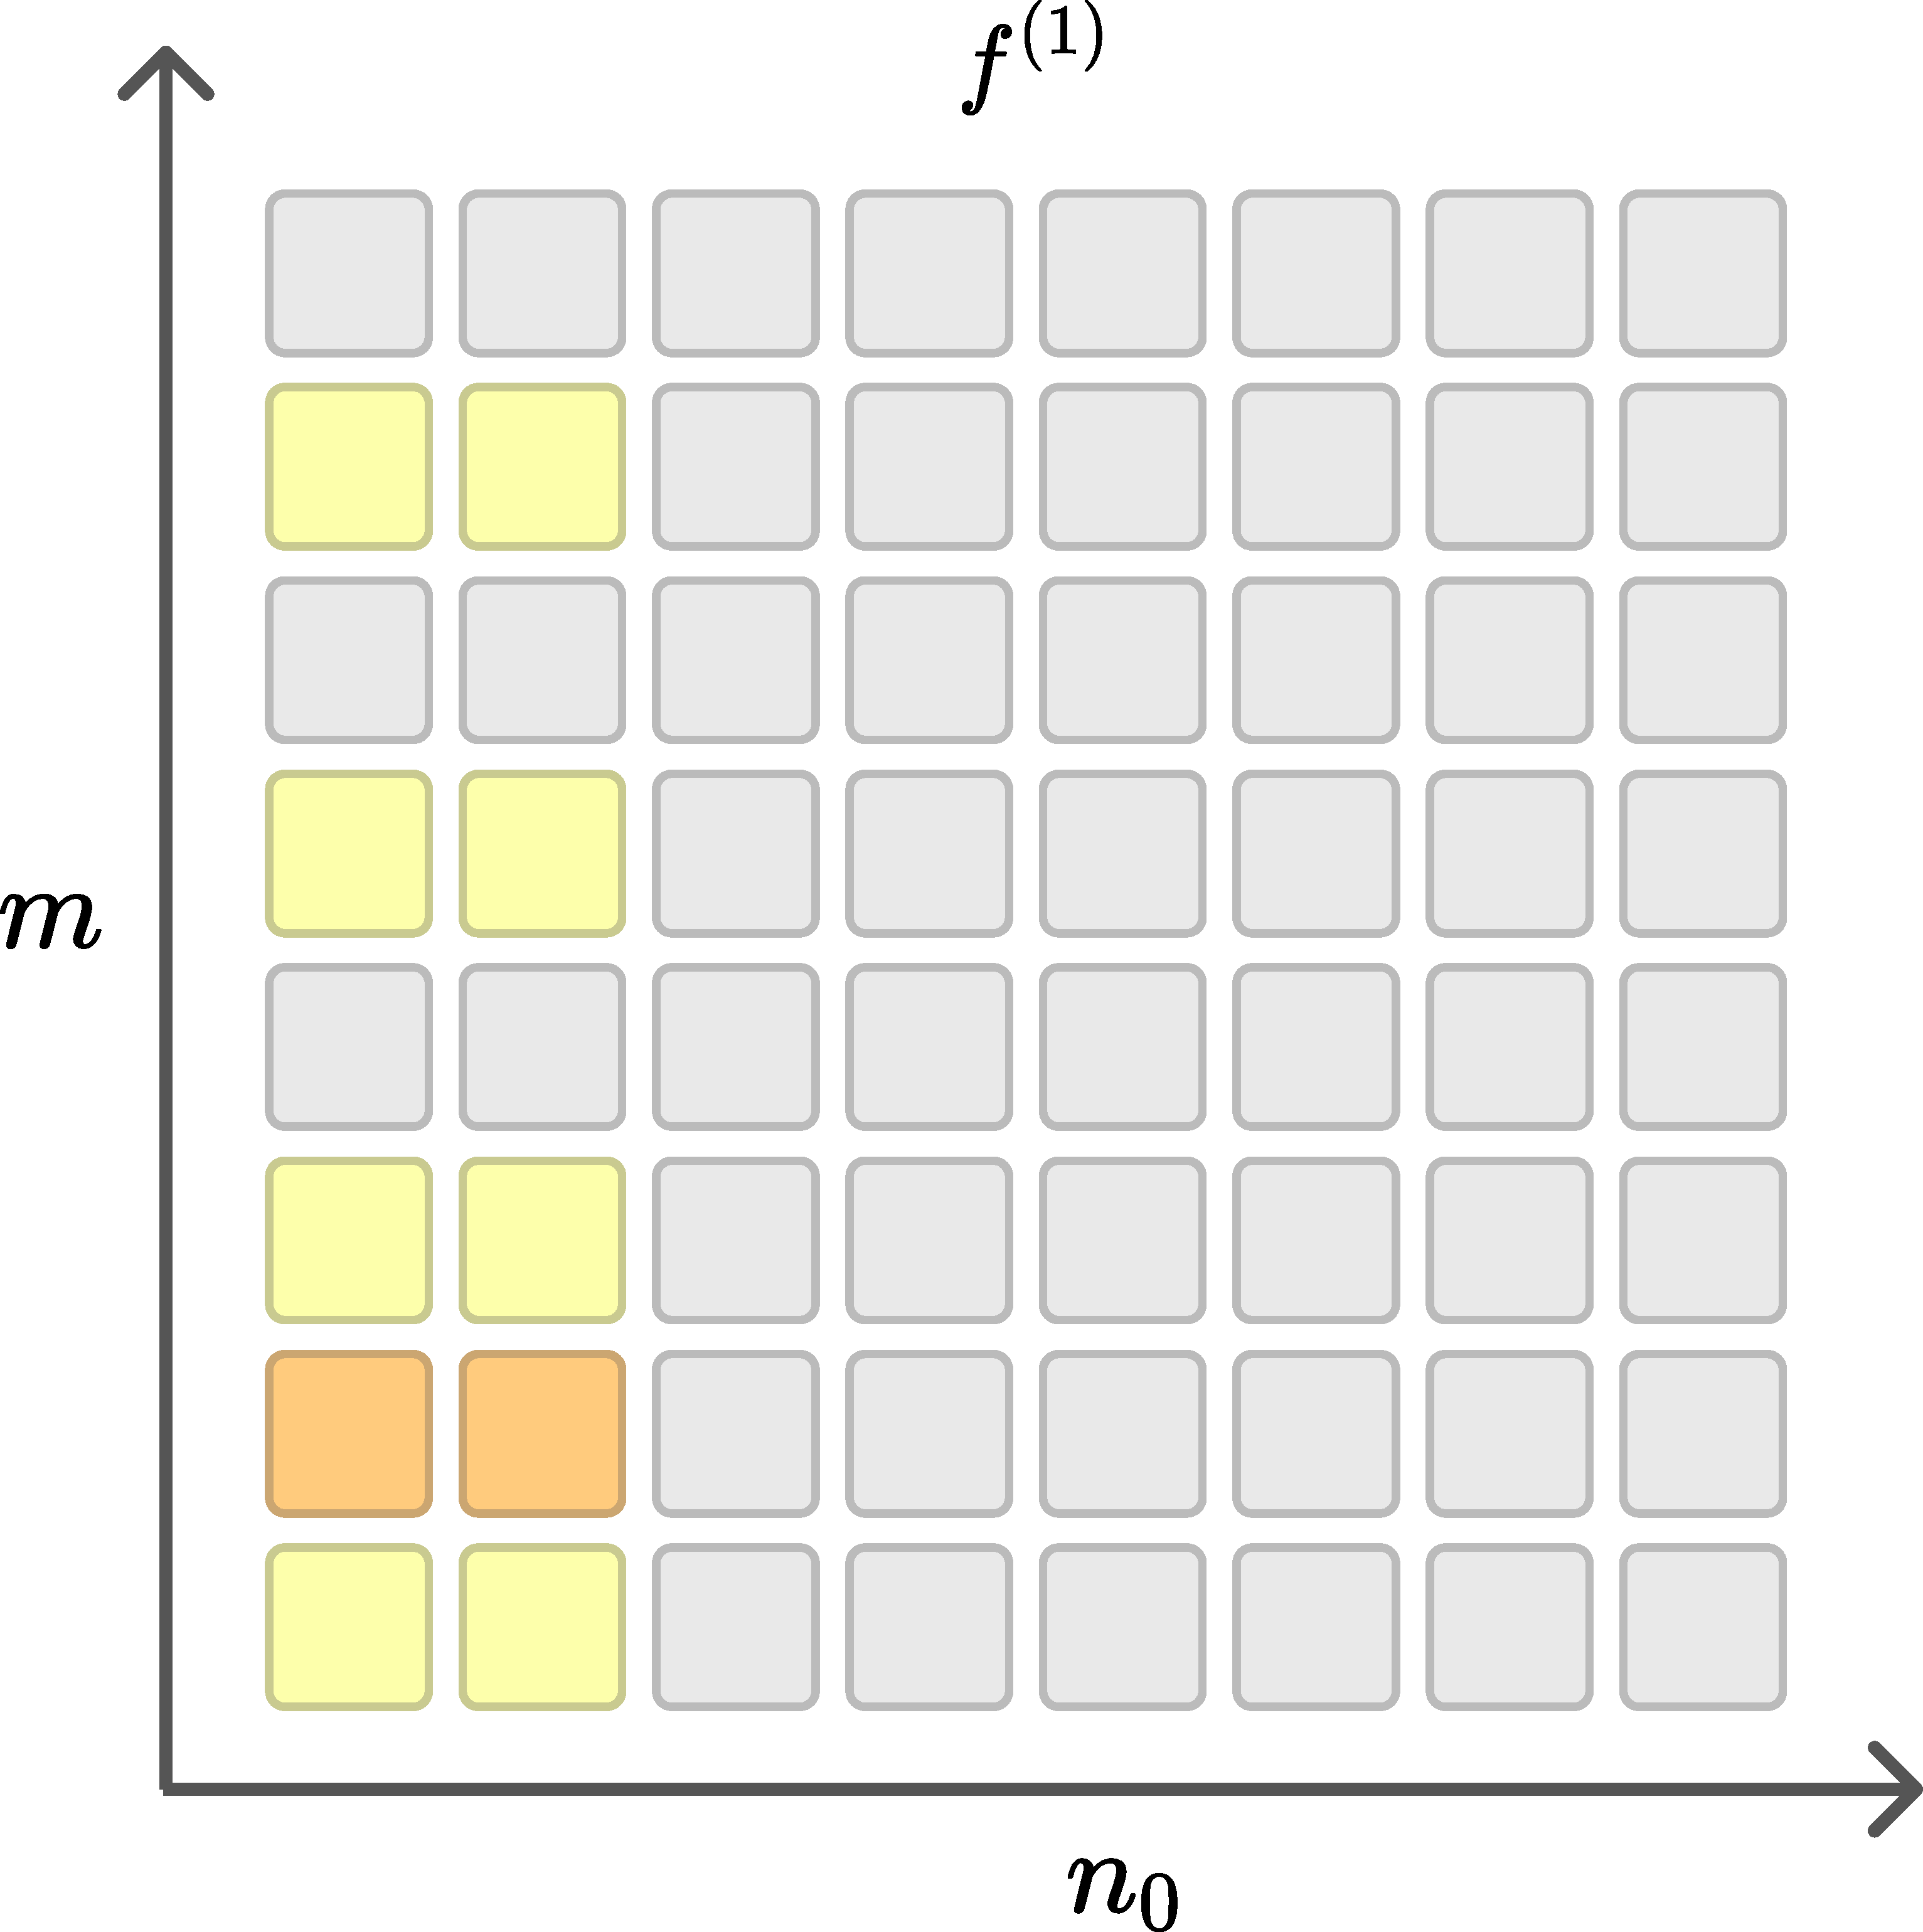
\includegraphics[width=0.30\textwidth]{tres.pdf}
    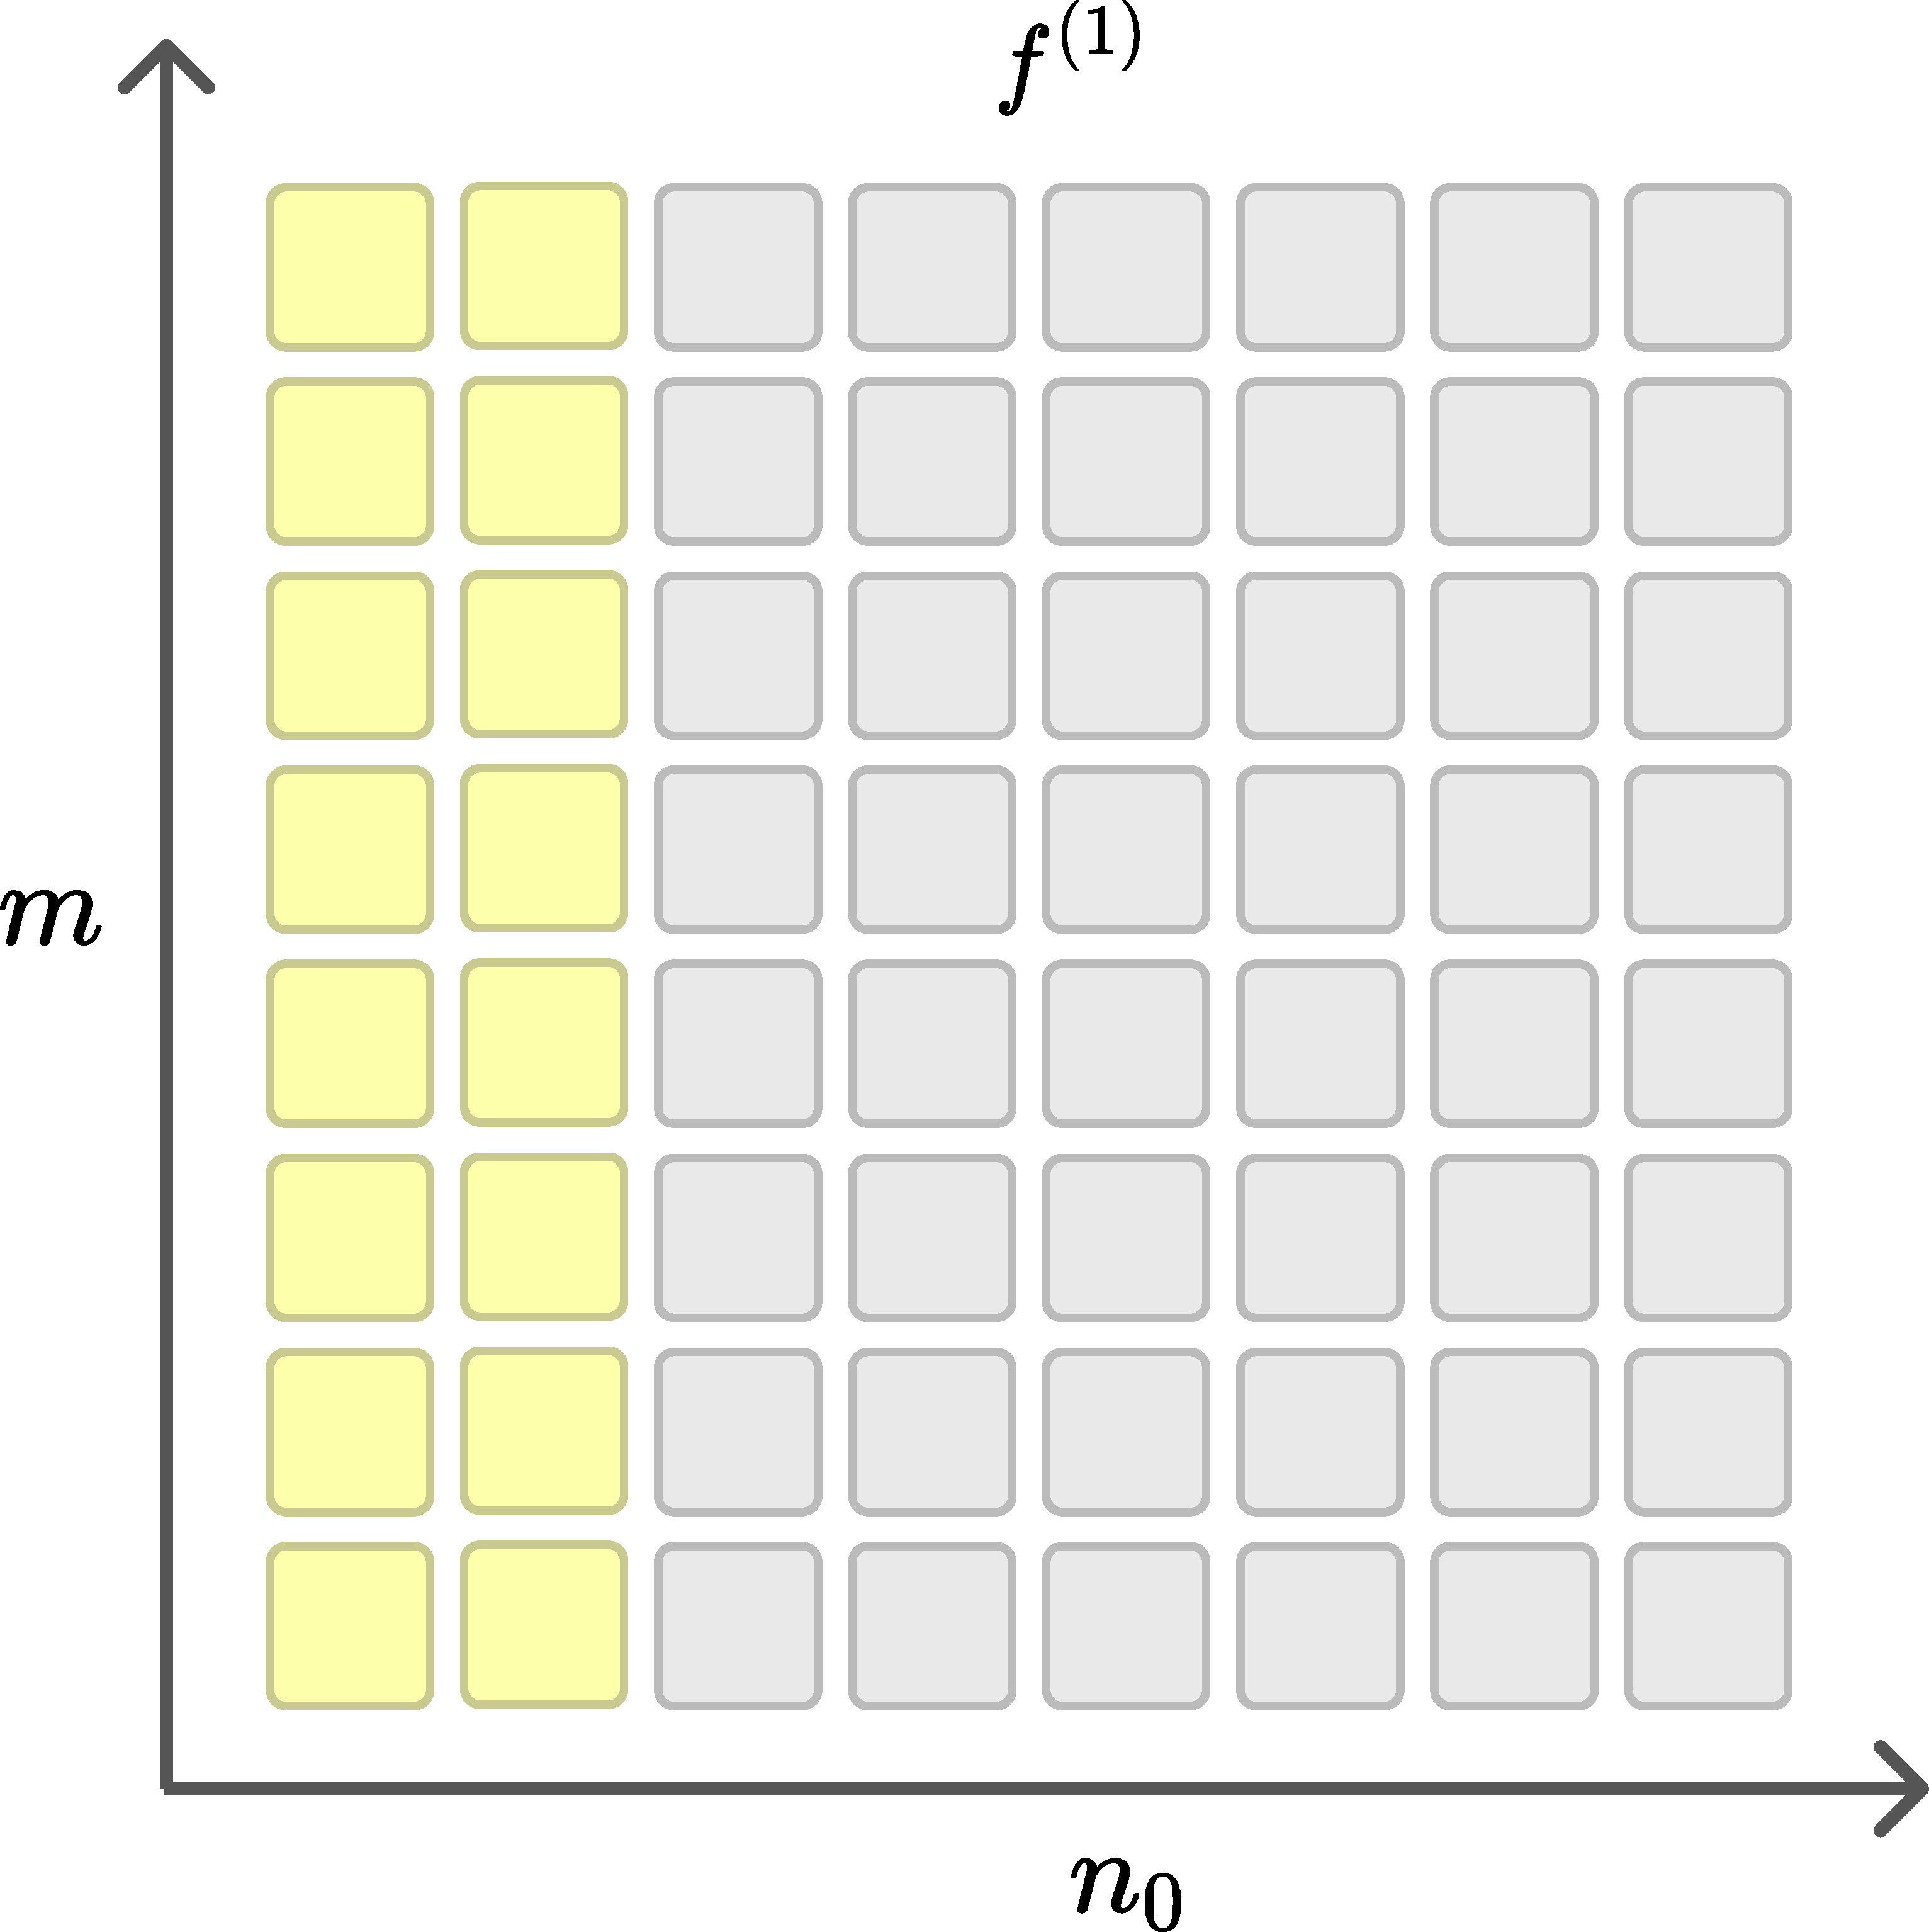
\includegraphics[width=0.30\textwidth]{quatro.pdf}
    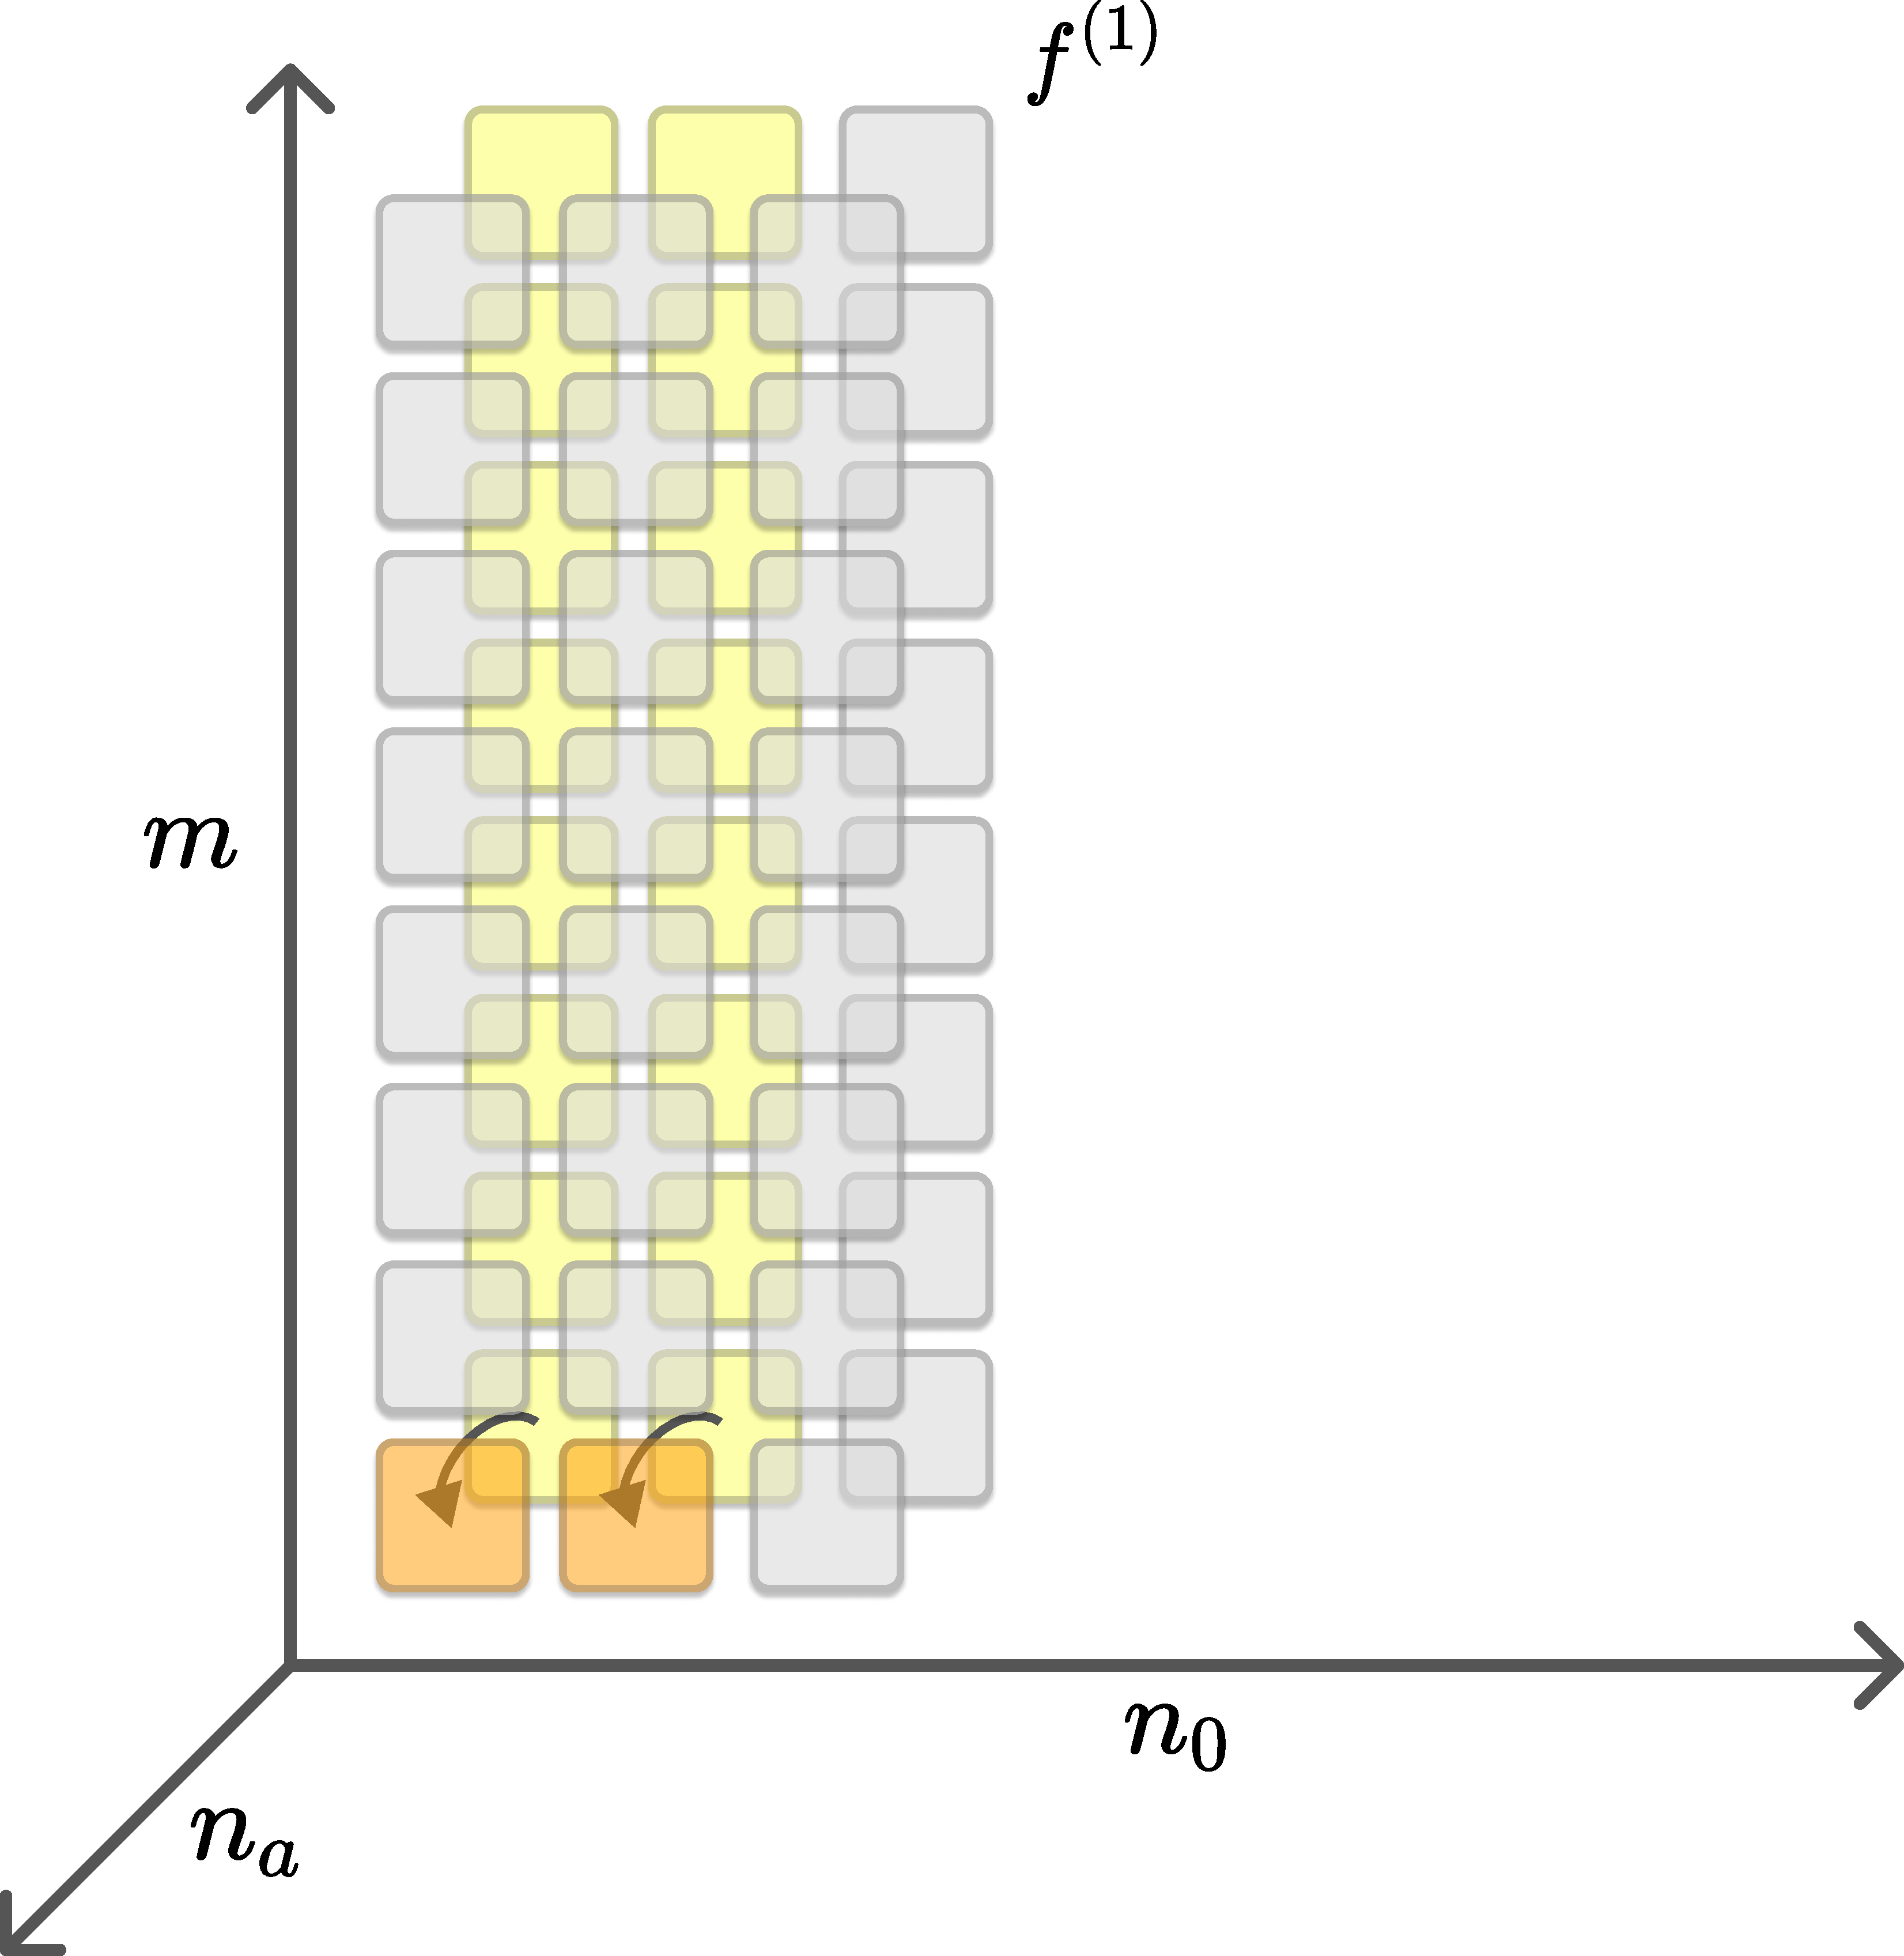
\includegraphics[width=0.30\textwidth]{cinco.pdf}
    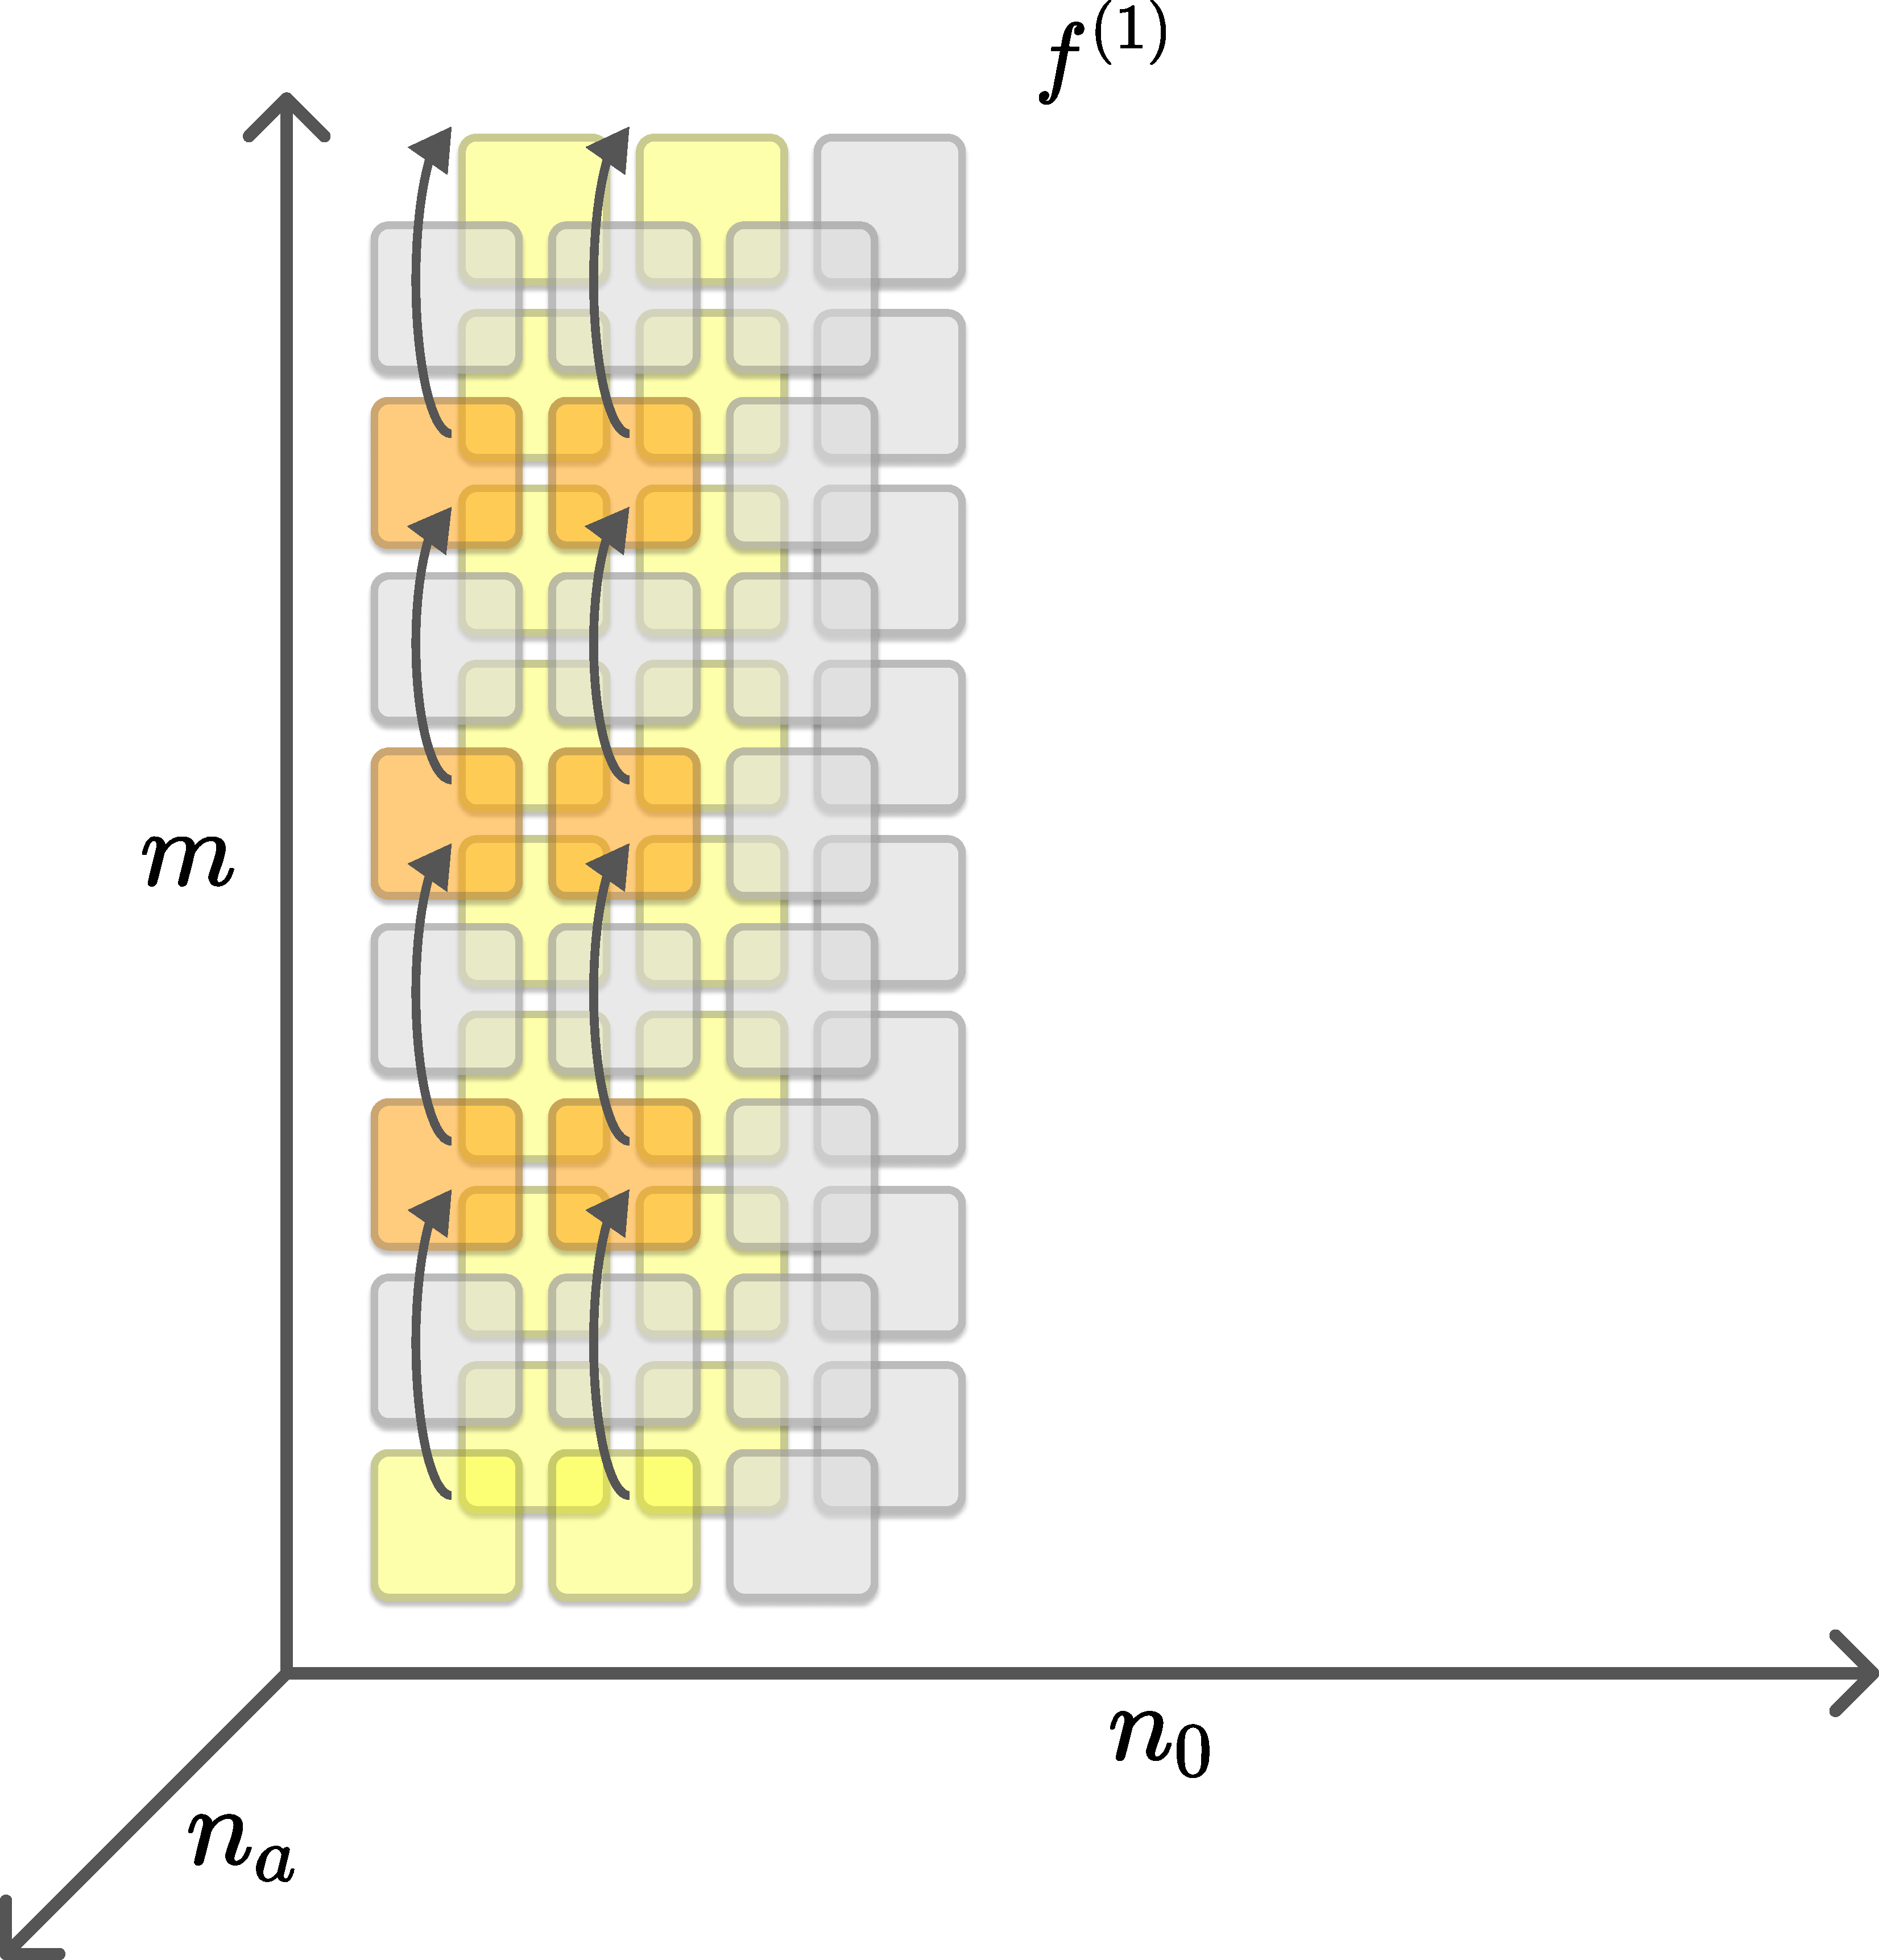
\includegraphics[width=0.30\textwidth]{seis.pdf}
    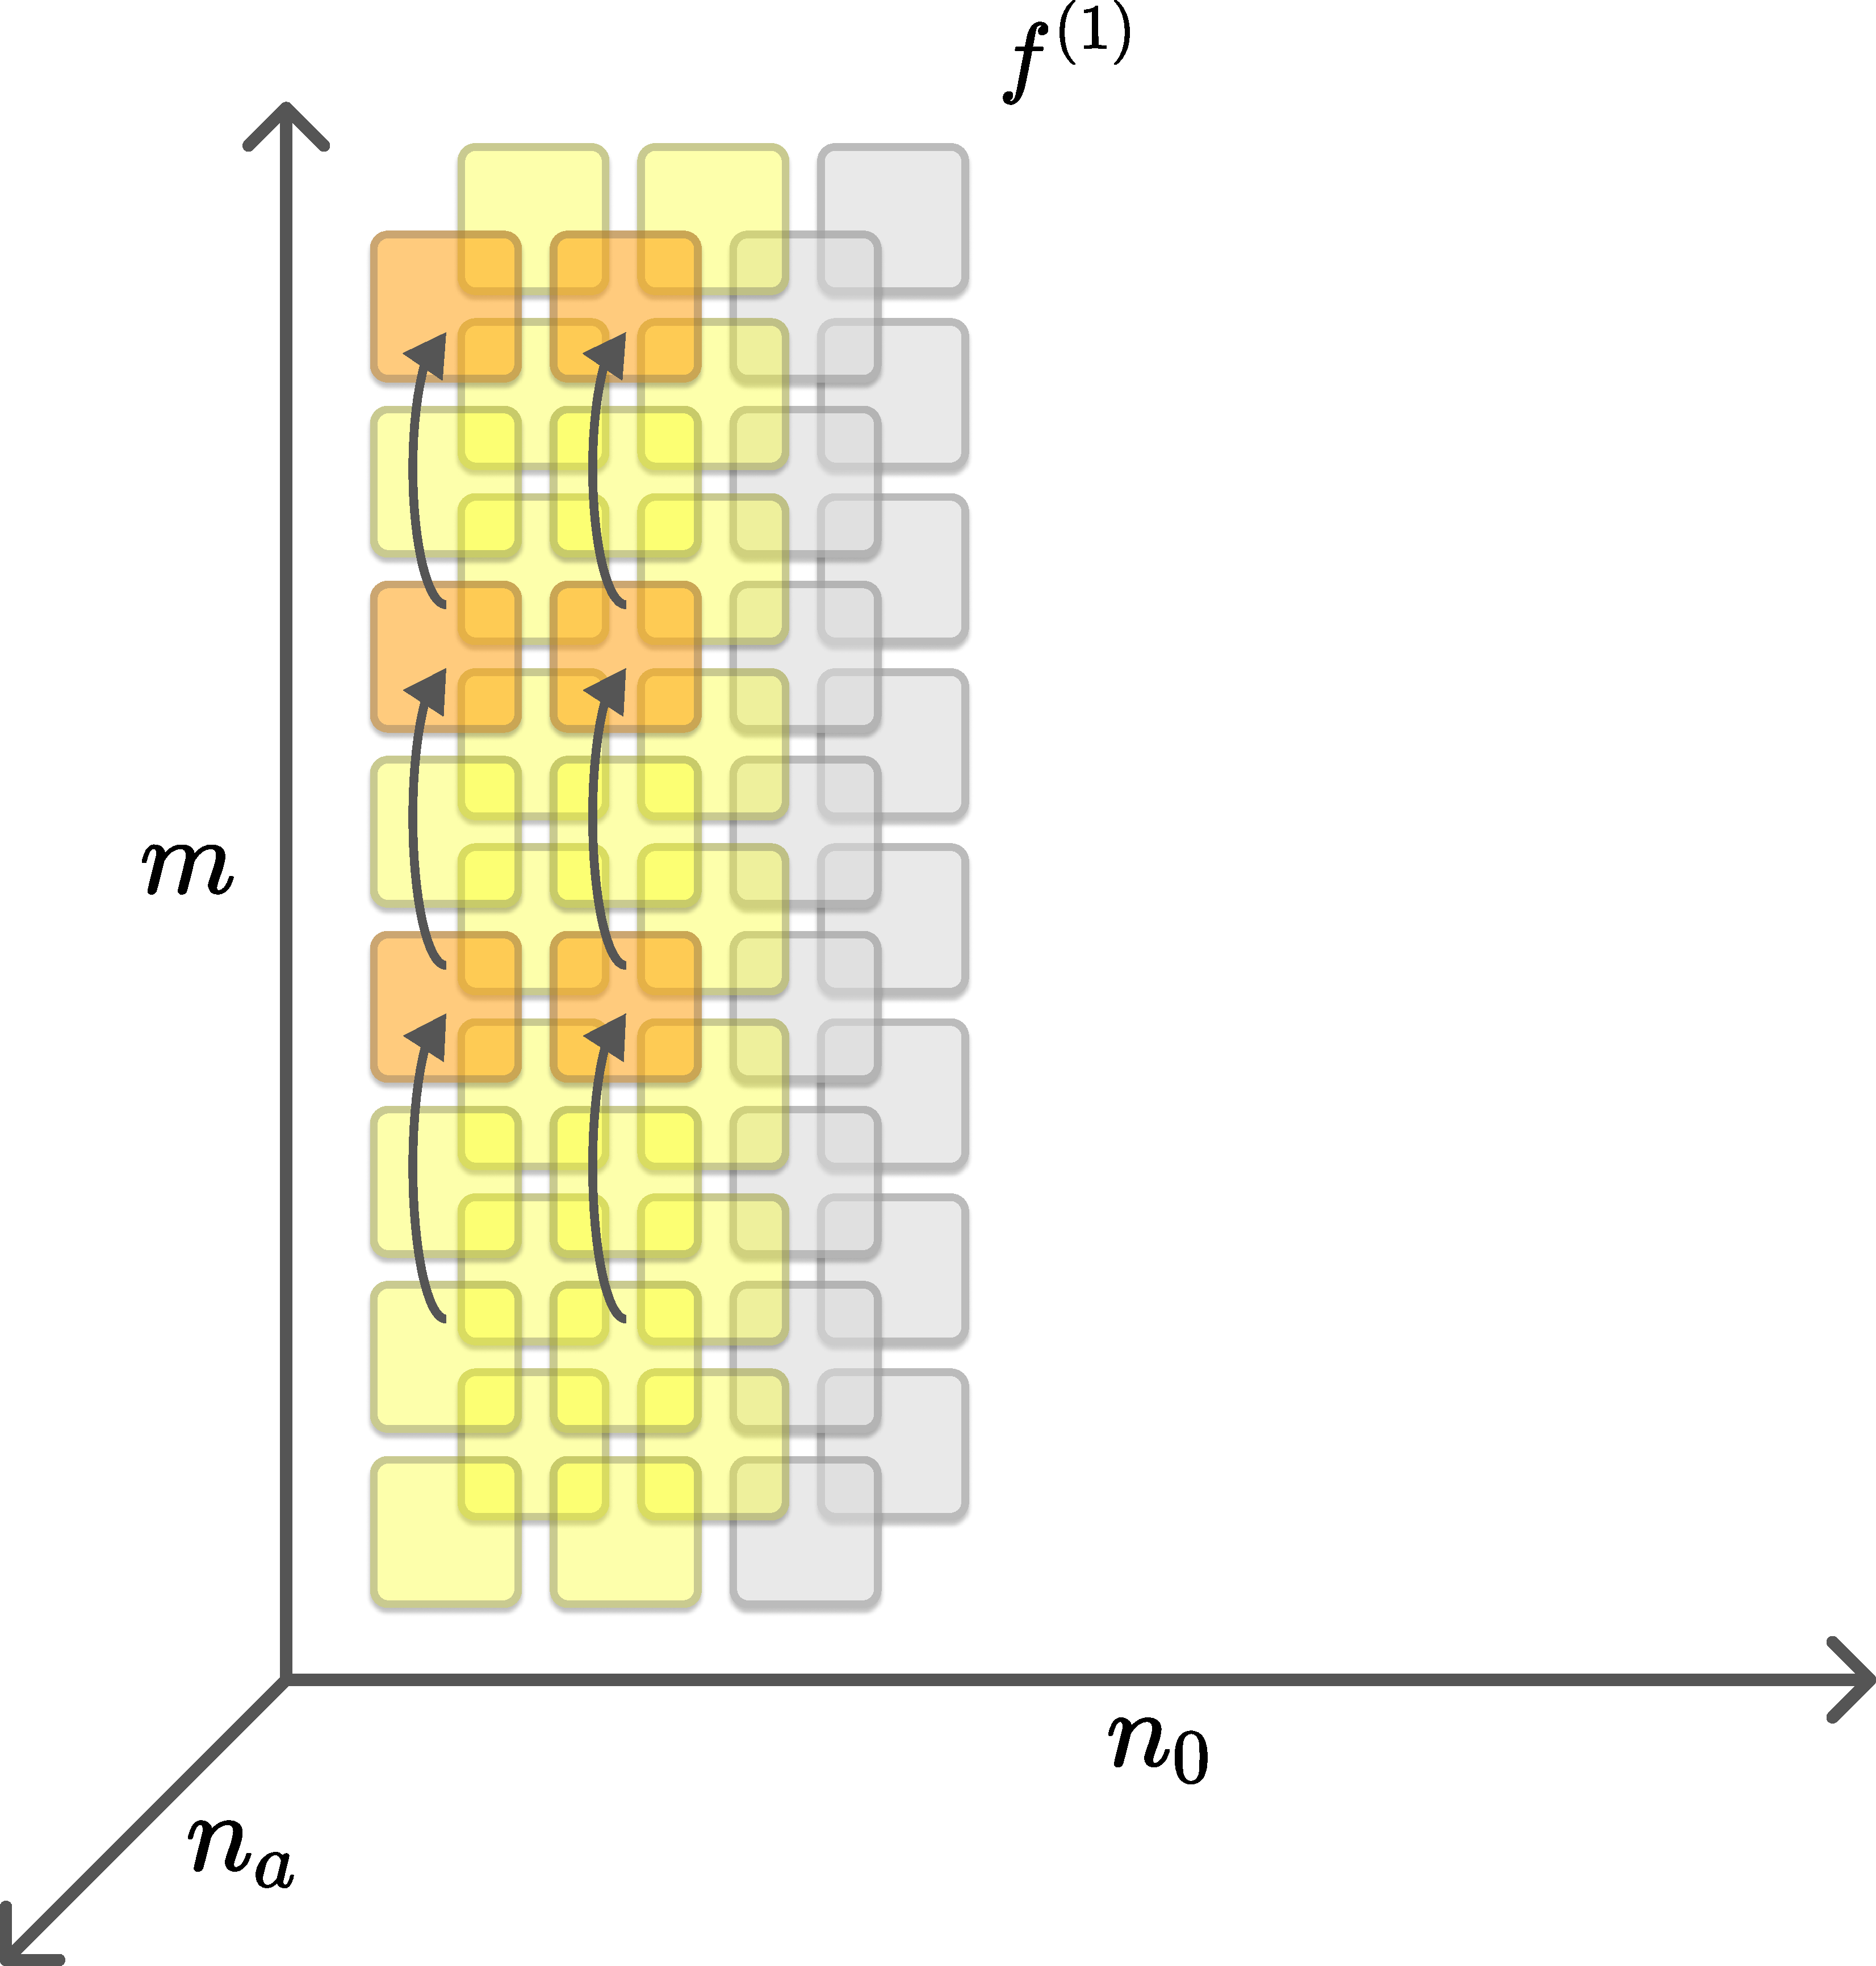
\includegraphics[width=0.30\textwidth]{ocho.pdf}
    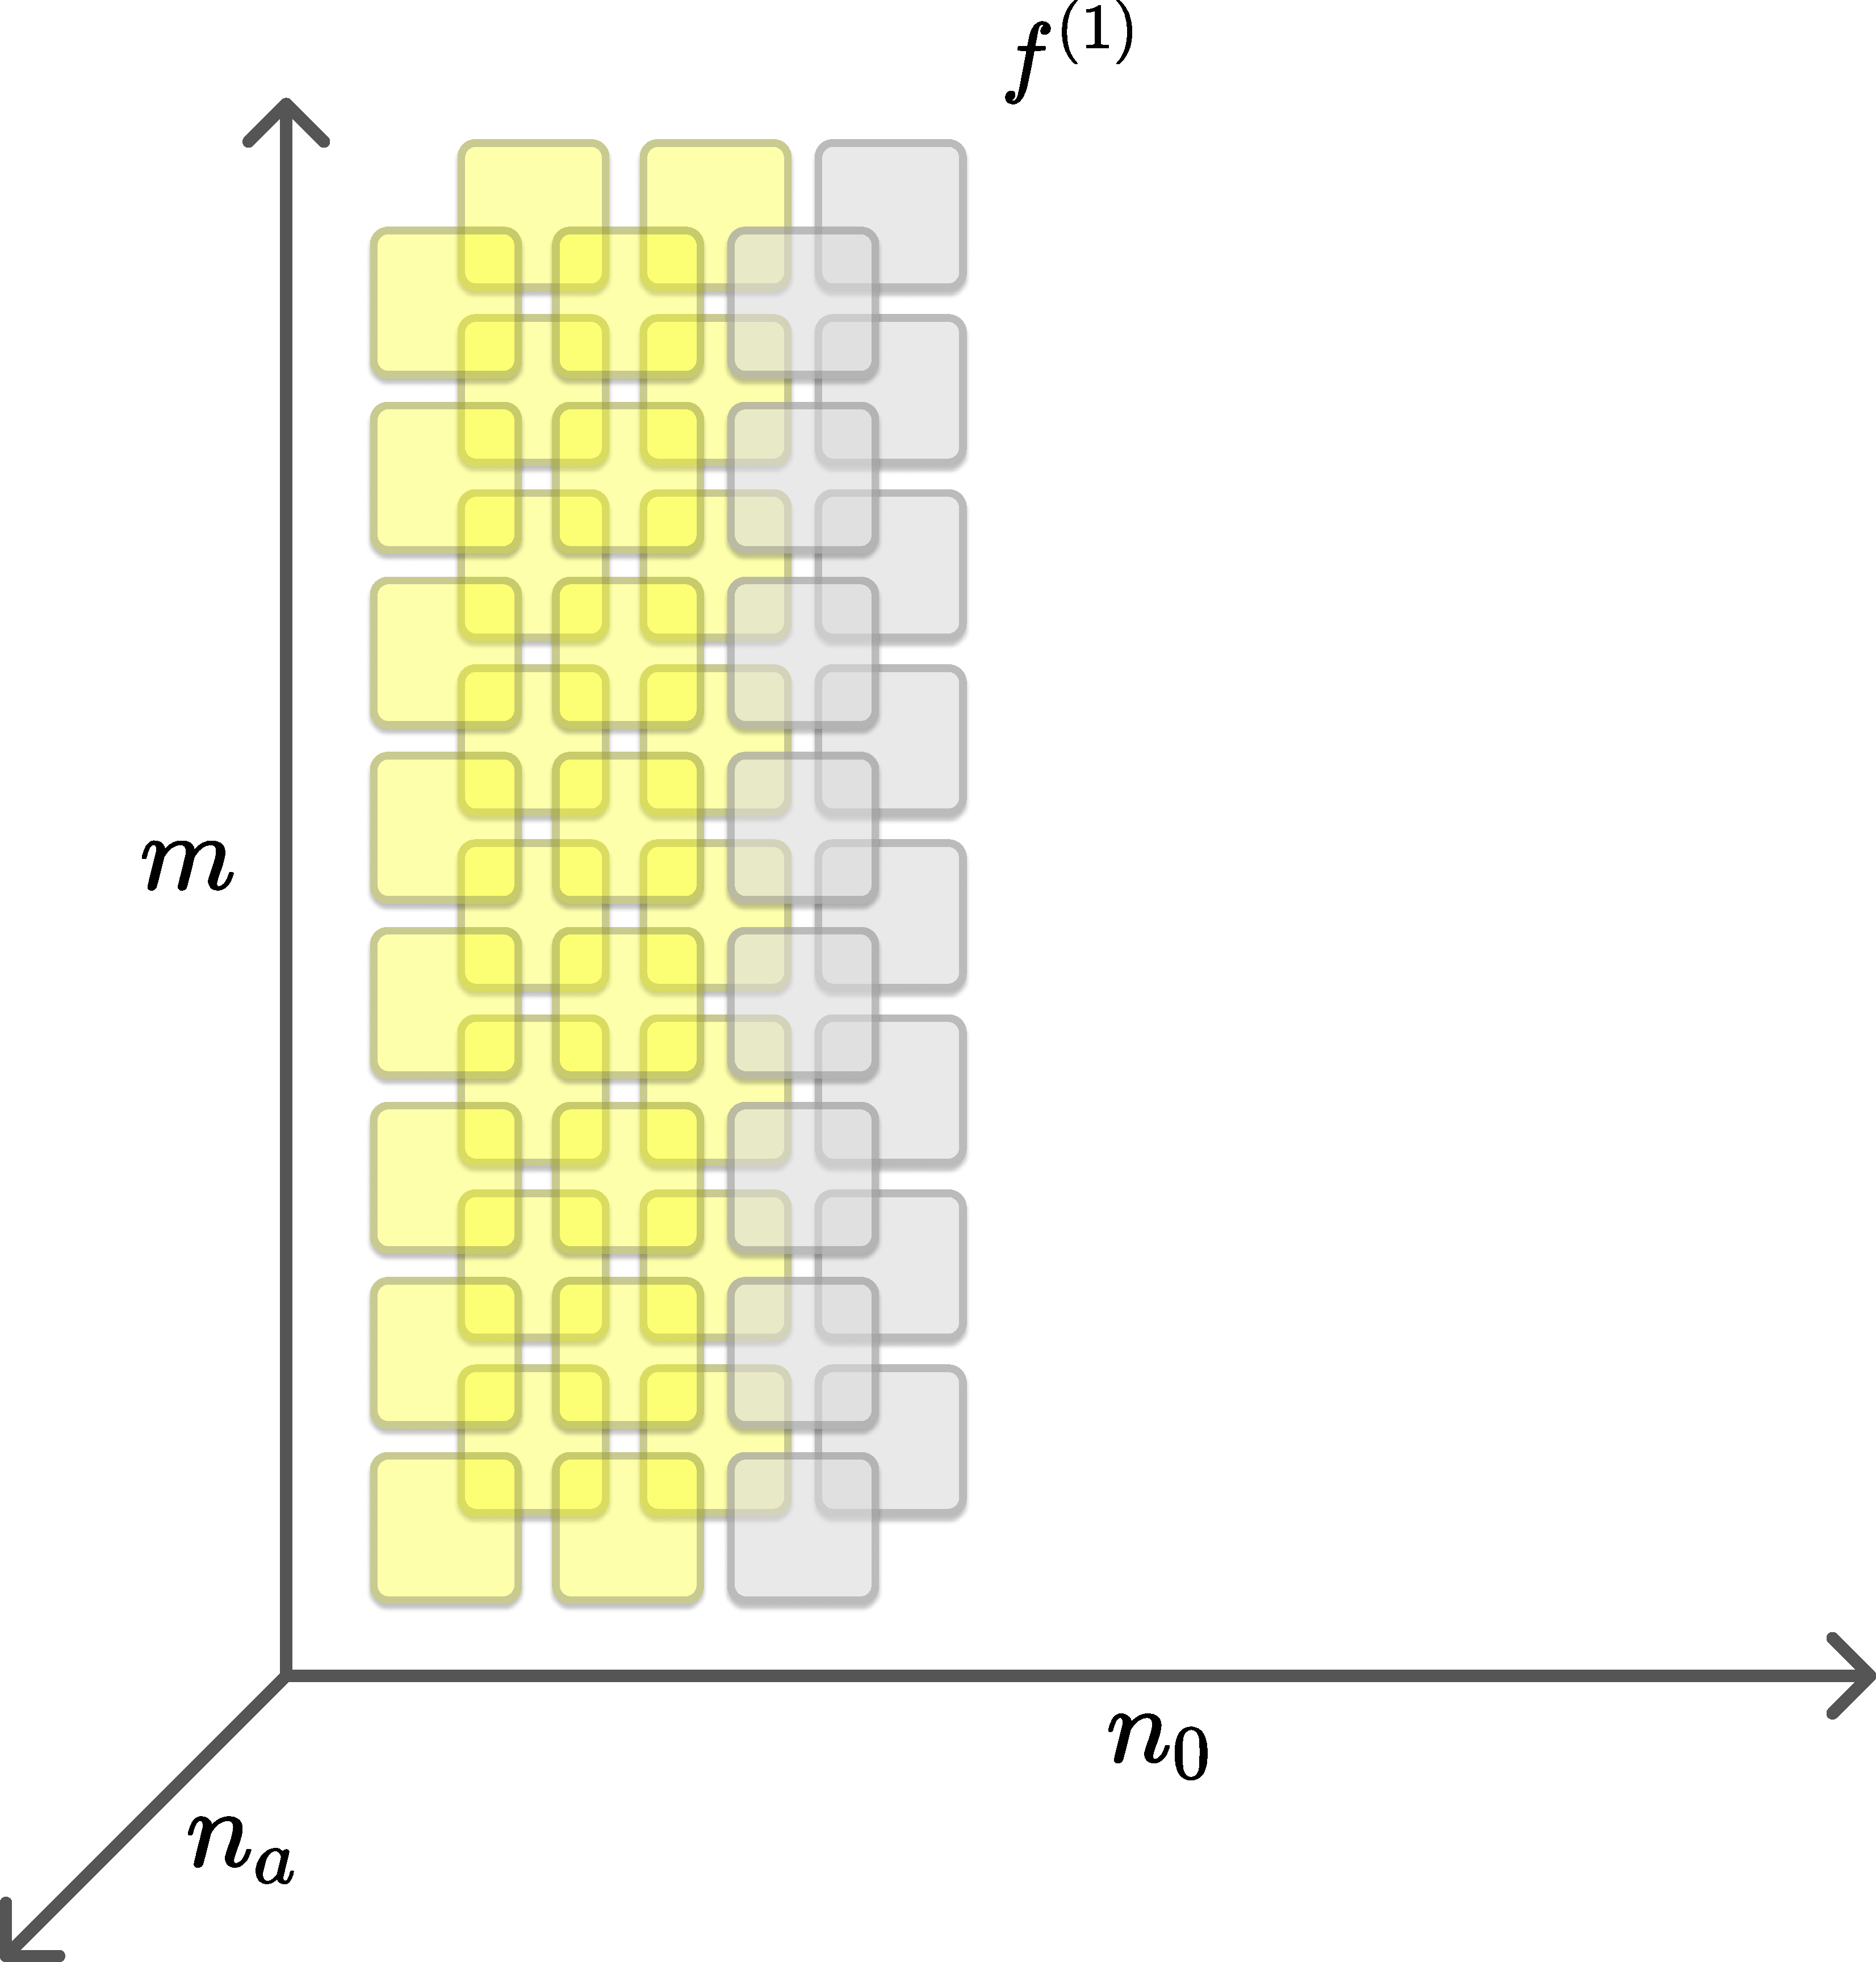
\includegraphics[width=0.30\textwidth]{nueve.pdf}
    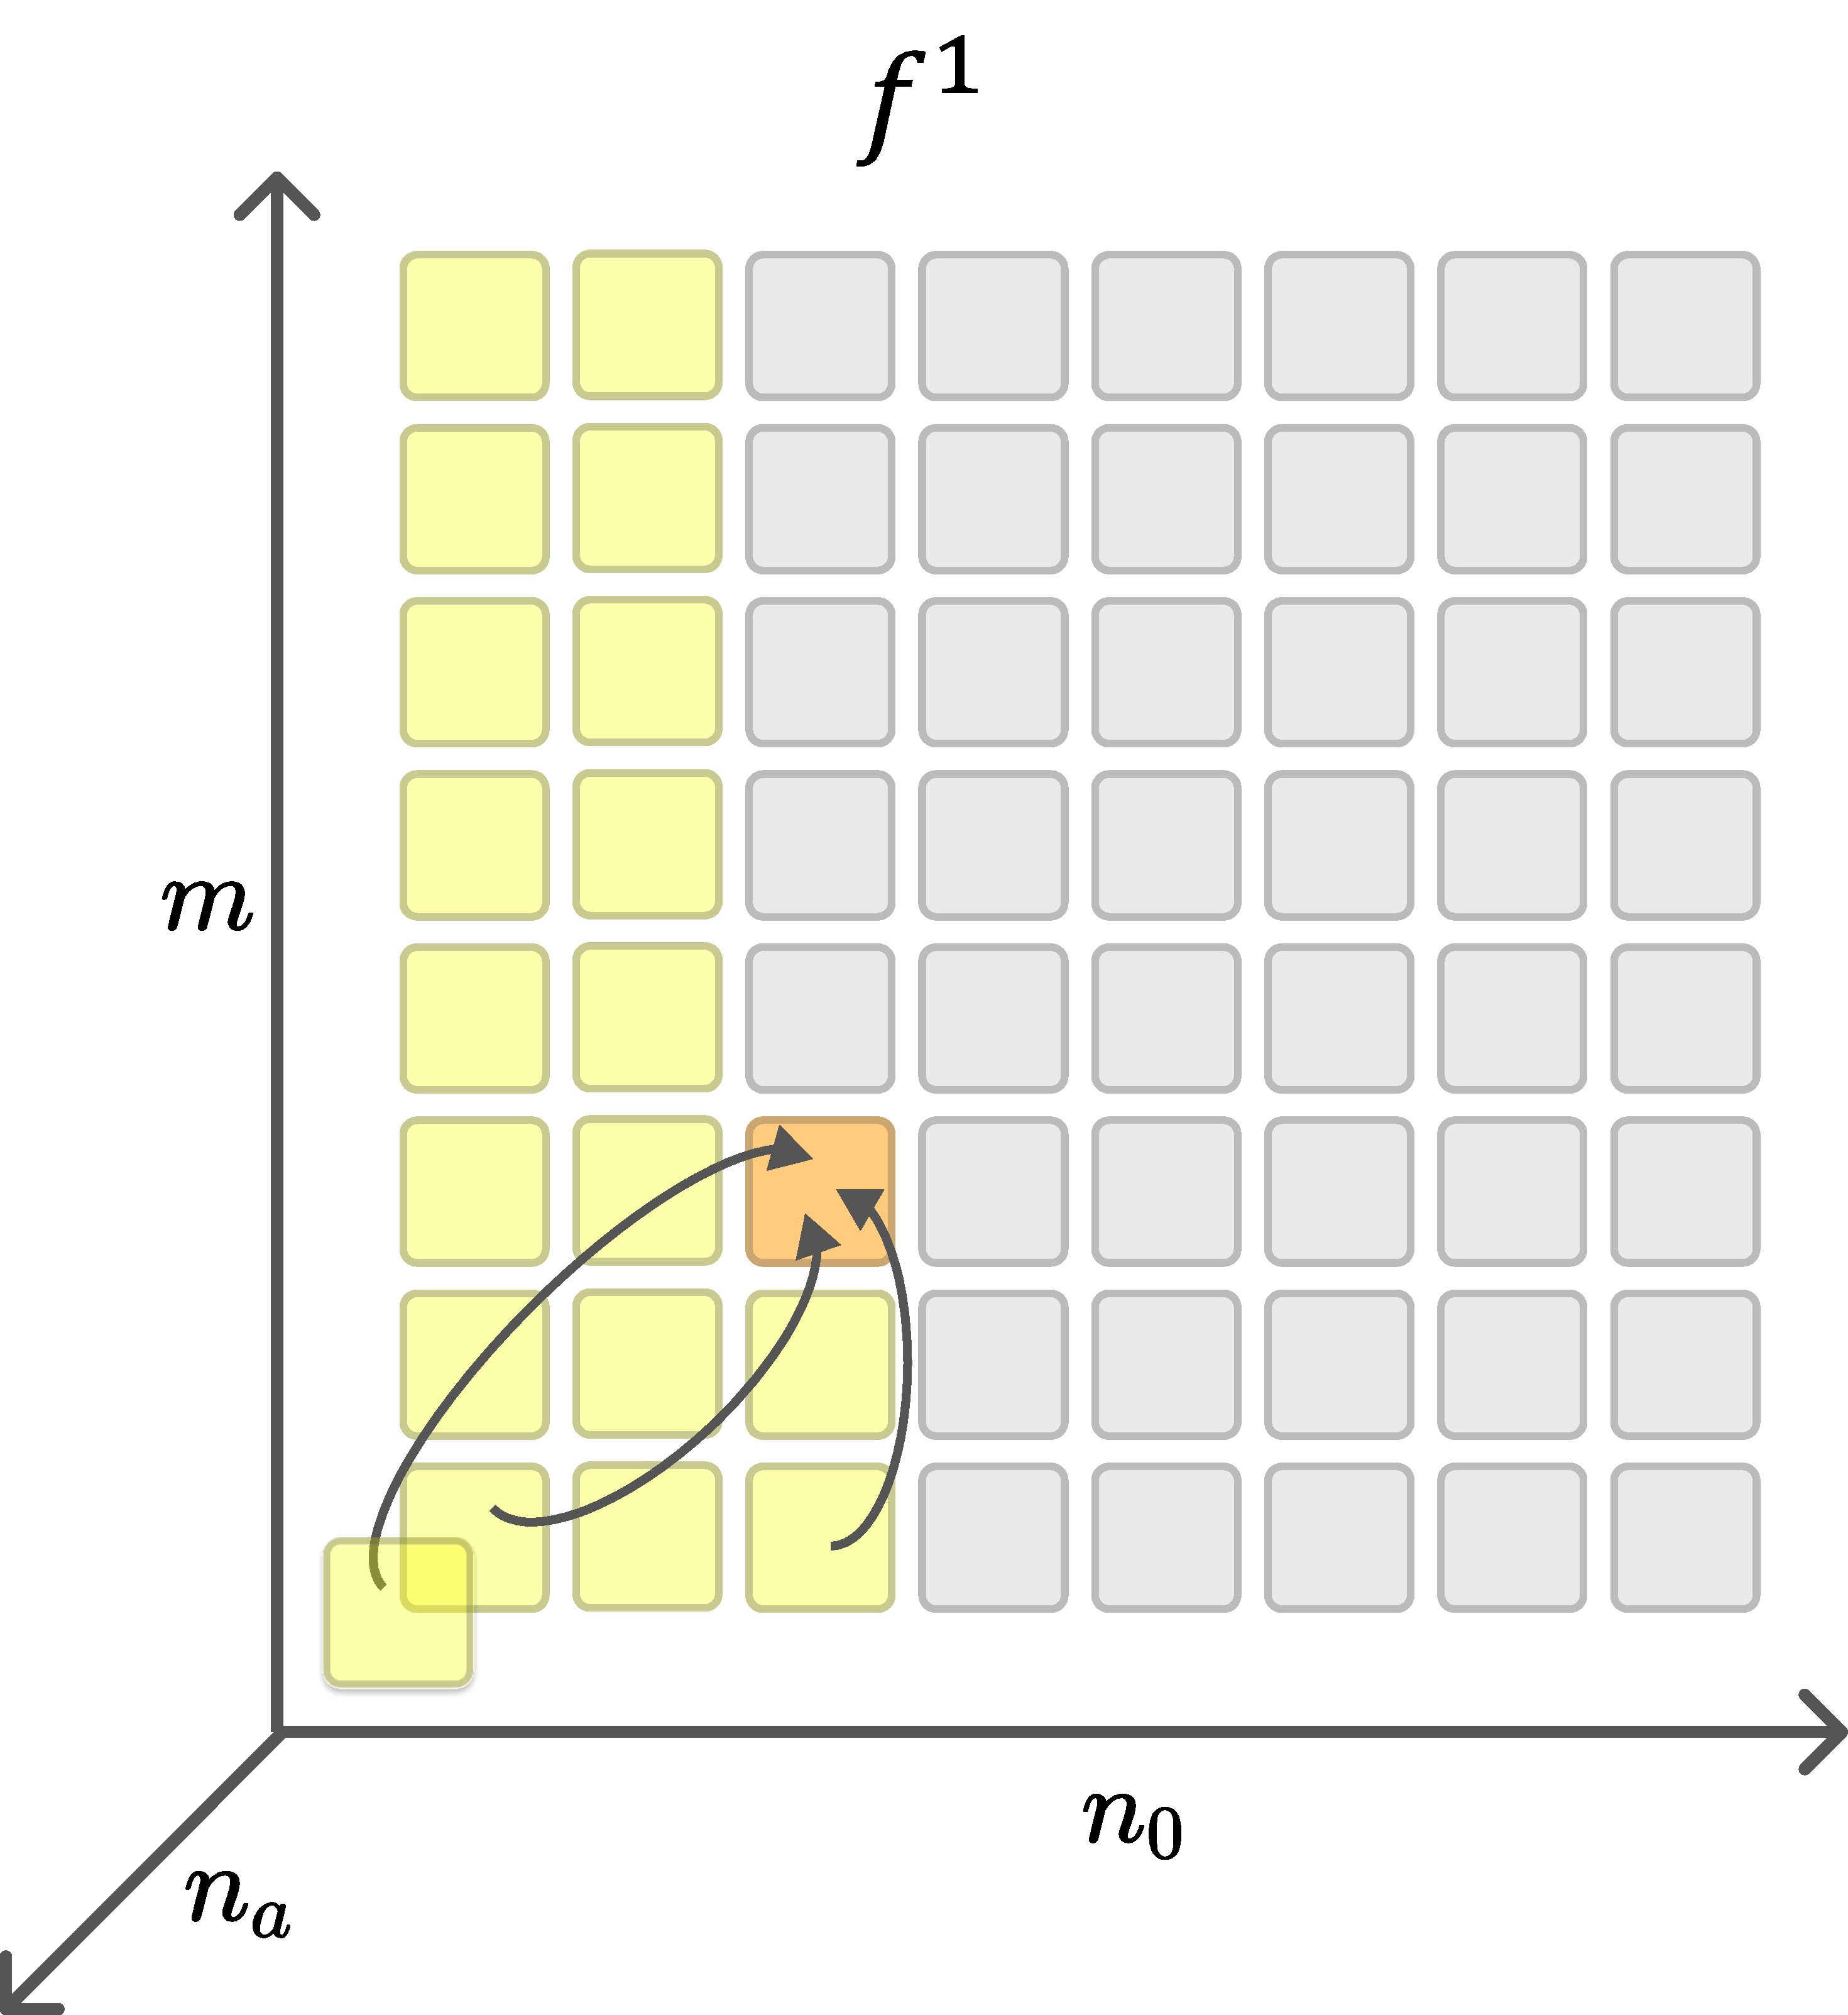
\includegraphics[width=0.30\textwidth]{Picture1.pdf}
    \caption{Approximate representation of the recursive relationship in f parameters}
    \label{recu}
\end{figure}

The closed analytical form of the master integral \ref{MasInt} is not known. However, Its value, and by extension values of other $f$ functions, can be effectively calculated with arbitrarily large precision by analyzing the behavior of its Taylor expansion.

When expanded into a series the master integral \ref{MasInt} takes the form \cite{metoda}:

\begin{equation}
    f\left(r\right) = \sum_{m=1}^{\infty}{\left[f_{m}^{(1)}\left(ln\left(r\right)+\gamma_E\right)+f_{m}^{(2)}\right]}
    \label{taylor}
\end{equation}
Here $\gamma_E$ represents the Euler constant, and parameters $f_{n}^{(1)}$ and $f_{n}^{(2)}$ are real constants. 

As shown in \cite{metoda} there exists a recursive relationship between the $f$ constants. Considering their relationship with the master integral recursive equations describing analogous parameters in the Taylor expansion of other $f$ functions can be obtained. The specific derivation of these relationships is beyond the scope of this thesis, but the approximate representation of these recursive relation for the parameter $f_{n}^{(1)}$ is presented on figure \ref{recu}.  

Initially all the $n$ parameters aside form $n_0$ are fixed at zero. Values of  $f_{1}^{(1)}(n_0 = 0)$ and $f_{1}^{(1)}(n_0 = 1)$ are then computed numerically. After that every value of $f_{m}^{(1)}(n_0 = 0)$ and $f_{m}^{(1)}(n_0 = 1)$ can be computed. After that values for $f_{2}^{(1)}(n_0 = 0 ; n_0 = 1)$ are computed, allowing one to fill in the missing values for $f_{1;2}^{(1)}(n_0 = 0 ; n_0 = 1)$. Using a different recursive relation the values of $f_{1}^{(1)}\left(n_{\left(n_1,n_2,n_3,n_4\right)} = 1\right)$ can be obtained. An analogous process to the one used for $f_{m}^{(1)}(n_0 = 1)$ can then be used to calculate the values of $f_{m}^{(1)}\left(n_{\left(n_1,n_2,n_3,n_4\right)} = 1\right)$. At that point yet another recursive relation allow one to calculate the values of the rest of the $f^{(1)}$ parameters. Only after calculating all the required $f^{1}$ values one can start calculating values of $f^{2}$, as the relationships describing them depend on $f^{1}$.

After all the required numeric values of $f^{(1)}$ and $f^{(2)}$ are calculated the approximated value of the $f$ functions can be easily obtained by plugging said coefficients into the previously defined series \ref{taylor}

\chapter{H2SOLV}
\label{h2solv chapter}

H2SOLV\cite{H2SOLV} is a piece of software allowing one to perform precise numerical calculations of two-electron diatomic systems

\section{Algorithmic description of the program}

The program in question implements the method described in chapter \ref{rob} allowing one to perform calculations of expected values of operator in two-electron diatomic molecules in a streamlined and efficient fashion. 

The program performs numerically calculates the value of each of the $f$ functions, so working with a full basis is impossible. 

In order to make the calculations feasible, a parameter bounding the number of functions comprising the given subset of a full basis is introduced. It will further be denoted as $\Omega$.  The subbasis defined by $\Omega$ will consist of functions $\psi_{n_0 n_1 n_2 n_3 n_4}$ for which

\begin{equation}
    \Omega \geq n_0+n_1+n_2+n_3+n_4
    \label{omegaDef}
\end{equation}

The program takes the distance between the nuclei $r_{AB}$, the charge of each nucleus and $\Omega$ as input

The program can operate in two modes: in the first one it uses the simplex method to optimize the non-linear parameters $y$, $x$, $u$ and $w$, therefore defining an optimal basis for the given system. It tries to find a combination of those values that gives the lowest energy for a given value of $r_{AB}$.

The second mode allows it to use the previously computed parameters to calculate the values of operators given to it during compilation. The operators are fed to the program in the form of equations defining their matrix represented in the $f$ function formalism.

Allowing all the non-linear parameters to be fully independent of one another might in some cases prove to be unpractical. For that reason the H2SOLV implements some special simplified methods for special degenerated basis

\section{James-Coolidge}

In this configuration the program assumes that parameters $x$ and $y$ are set to $0$. In that form the basis is equivalent to that first defined by James \& Coolidge \cite{JamesCoolidge}, hence the name. Here the basis functions degenerate to 

\begin{multline}
    \psi_{n_0 n_1 n_2 n_3 n_4} \left( r_{1A}, r_{1B}, r_{2A}, r_{2B}, r_{12} \right) = e^{-u\left(r_{1A}+r_{1B}\right)-w\left(r_{2A}+r_{2B}\right)}r_{12}^{n_0}{\left(r_{1A}-r_{1B}\right)}^{n_1}\\
    {\left(r_{2A}-r_{2B}\right)}^{n_2}{\left(r_{1A}+r_{1B}\right)}^{n_3}{\left(r_{2A}+r_{2B}\right)}^{n_4}
    \label{JC form}
\end{multline}

Here the exponential part of the functions depends on the sum of the distances of the electrons from each of the nuclei, ensuring that both nuclei can have a similar input into the final form of the wave function.

This configuration should allow the program to effectively optimize the basis in configurations where the nuclei are placed relatively close to each other.

\section{Ionic}

In this configuration the program assumes that $x=y$ and $u=v$. Therefore, the basis functions degenerate to

\begin{multline}
    \psi_{n_0 n_1 n_2 n_3 n_4} \left( r_{1A}, r_{1B}, r_{2A}, r_{2B}, r_{12} \right) = e^{-2x\left(r_{1A}+r_{2A}-r_{1B}-r_{2B}\right)-2u\left(r_{1A}+r_{1B}+r_{2A}+r_{2B}\right)}\\
    r_{12}^{n_0}{\left(r_{1A}-r_{1B}\right)}^{n_1}{\left(r_{2A}-r_{2B}\right)}^{n_2}{\left(r_{1A}+r_{1B}\right)}^{n_3}{\left(r_{2A}+r_{2B}\right)}^{n_4}
    \label{ionic form}
\end{multline}

It can be observed that if a constraint $x=u$ is also imposed the functions degenerate further to

\begin{multline}
    \psi_{n_0 n_1 n_2 n_3 n_4} \left( r_{1A}, r_{1B}, r_{2A}, r_{2B}, r_{12} \right) = e^{-4xr_{1A}-4ur_{2A}}\\
    r_{12}^{n_0}{\left(r_{1A}-r_{1B}\right)}^{n_1}{\left(r_{2A}-r_{2B}\right)}^{n_2}{\left(r_{1A}+r_{1B}\right)}^{n_3}{\left(r_{2A}+r_{2B}\right)}^{n_4}
    \label{ionic  degen form}
\end{multline}

In that case the exponential part of the function becomes dependent solely on the distance of the electrons from the first nuclei. In such state the base akin to a basis suitable for representing a single nucleus ion, hence the name.

The symmetry of this configuration should allow the program to effectively optimize the basis in configurations where the nuclei are placed relatively far apart.
\chapter{Electric dipole moment}

\begin{figure}[H]
    \center
    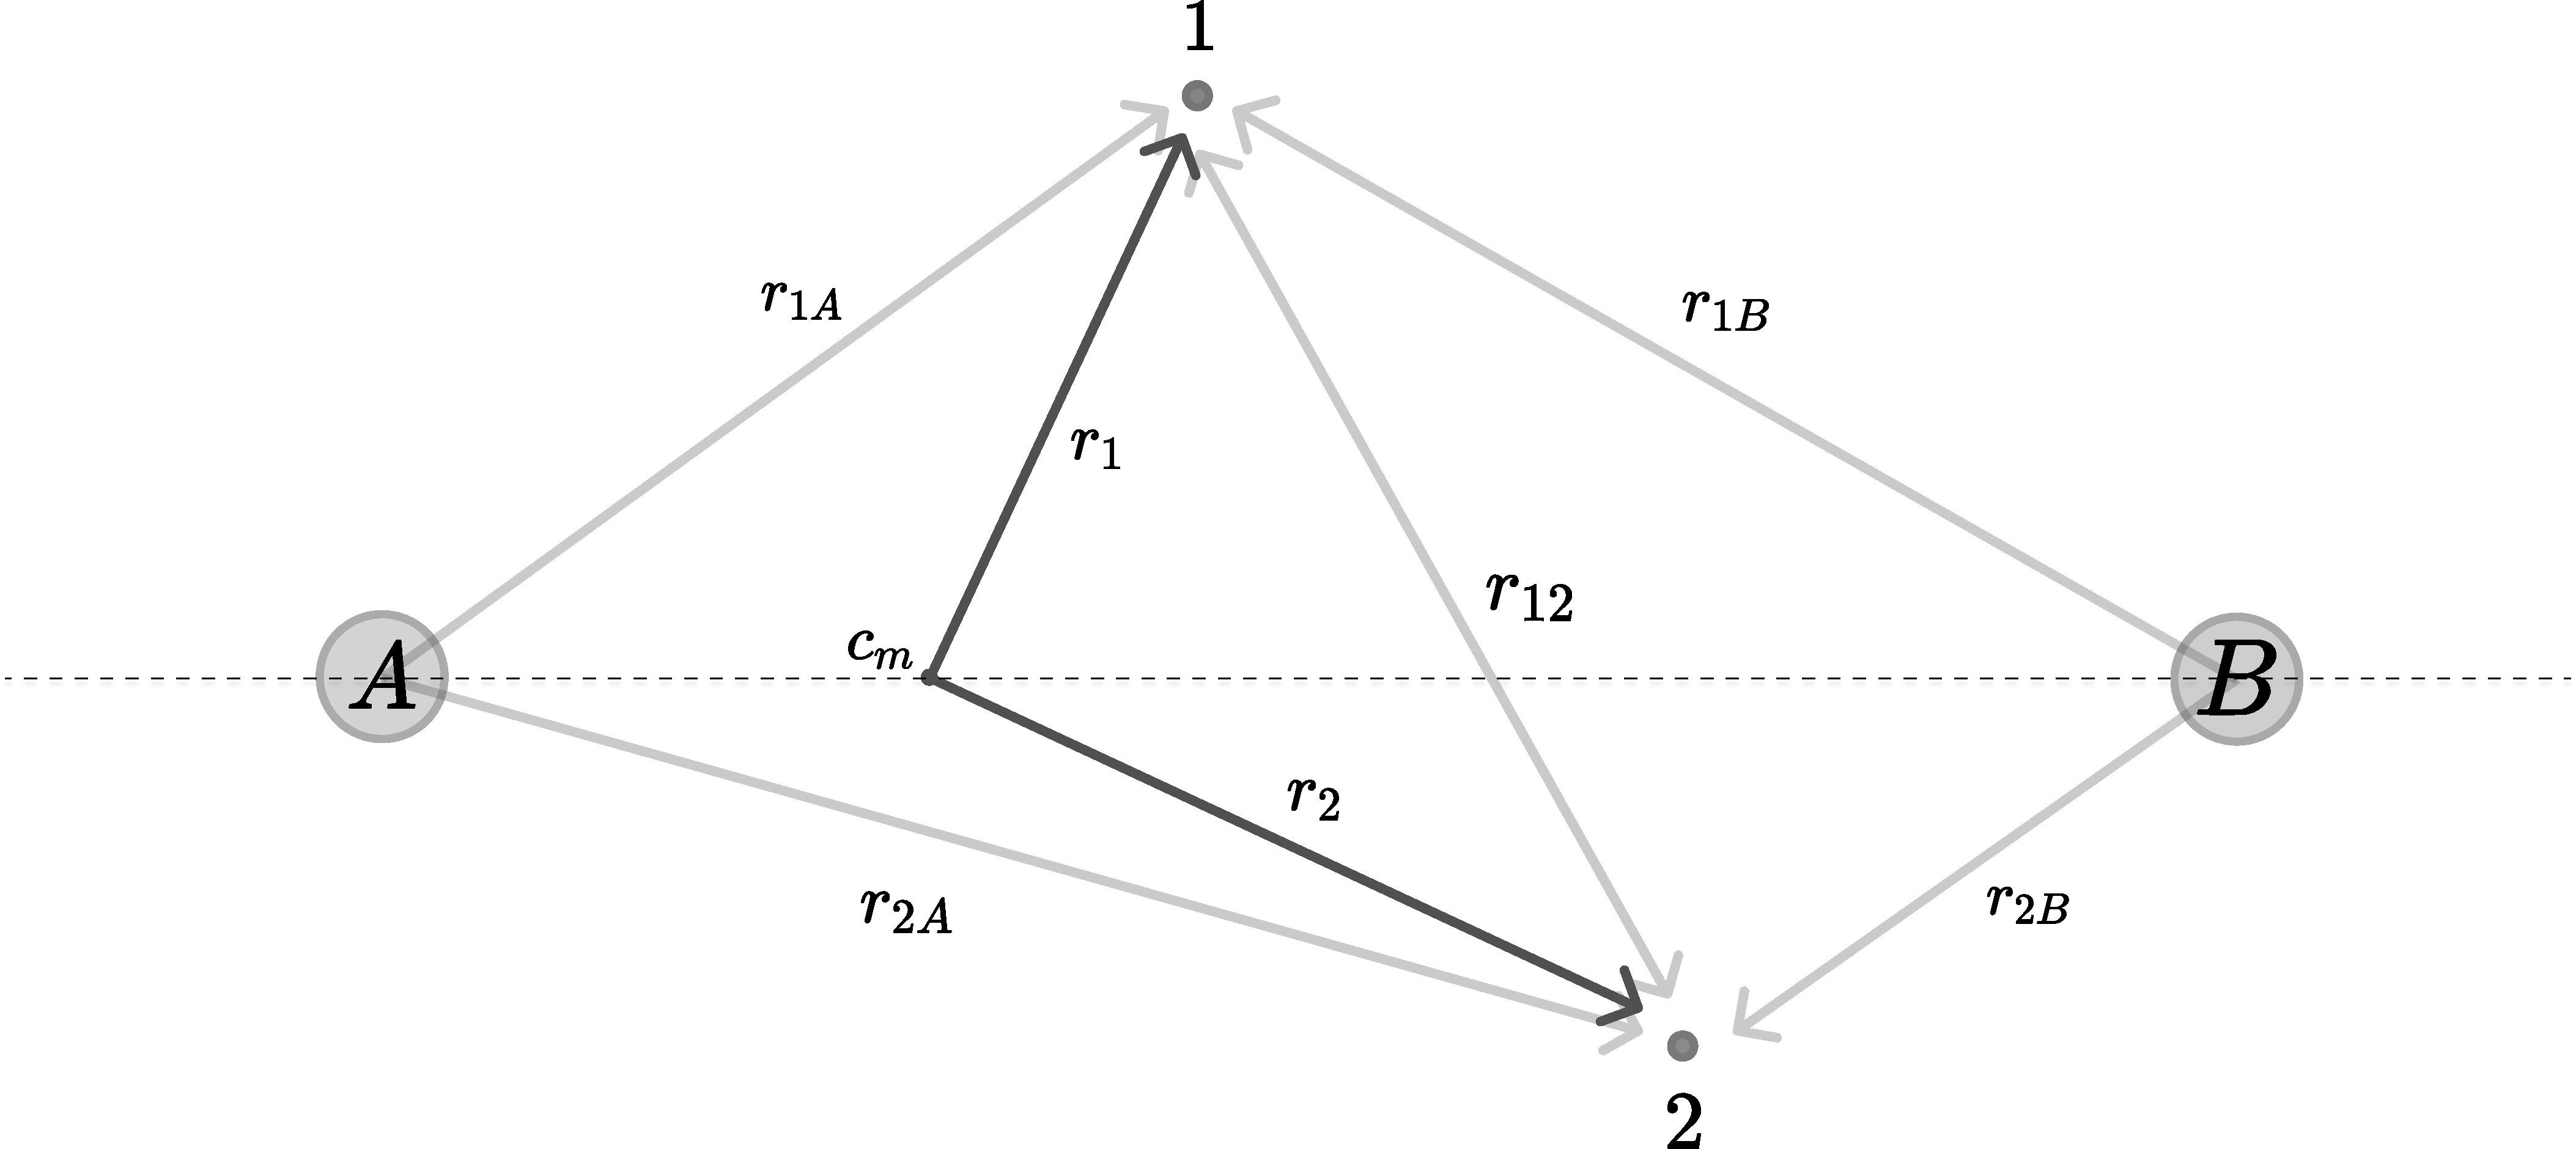
\includegraphics[width=0.6\textwidth]{systemVec.pdf}
    \caption{Visual representation of the system}
\end{figure}

Electric dipole moment of the charged particle is described by the operator $qr$, where $r$ is the position of the particle, and $q$ is its charge. Therefore, in the case of a two electron particle the 
permanent dipole moment between states $\Psi$ and $\Phi$, later referred to as $M$, is given by the formula \cite{Moper}
\begin{equation}
    \bra{\Psi}\left(\mathbf{r_1} + \mathbf{r_2}\right)\Ket{\Phi}
    \label{Meq}
\end{equation}

Here $r_1$ and $r_2$ represent the position of the two electrons

The above-mentioned formula \ref{Meq} can be restated in the previously defined formalism of $f$ function.

It can be observed that, due to the symmetry of the system, input to the permanent moment originating from the components of the position vector not parallel to the axis described by the nuclei will inevitably cancel out during integration. Therefore, during further calculations only the position vectors component parallel to the aforementioned axis will be taken into account. It will further be referred to as $r_z$. In turn operator \ref{Meq} is equivalent to 

\begin{equation}
    \bra{\Psi}\left({r_z}_1 + {r_z}_2\right)\Ket{\Phi}
    \label{MeqRz}
\end{equation}

Assuming the origin of the coordinates' system is placed in the center of mass of the two nuclei $r_z$ can be written as

\begin{equation}
    r_z = \frac{r_a^2 - r_b}{2r_{AB}} - \frac{M_a-M_b}{M_a + M_b}r_{AB}
    \label{rz}
\end{equation}

Therefore, the final form of the permanent electric moment in the f function formalism is given by

\begin{multline}
    M_{kl} = \left(\left(\left(f\left(1 + n_1,n_2,1 + n_3,2 + n_4,3 + n_5\right)\right.\right.\right. - \\
    f\left(1 + n_1,n_2,3 + n_3,2 + n_4,1 + n_5\right) + \\
    f\left(1 + n_1,1 + n_2,n_3,3 + n_4,2 + n_5\right) - \\
    f\left(1 + n_1,1 + n_2,2 + n_3,3 + n_4,n_5\right) - \\
    f\left(1 + n_1,2 + n_2,1 + n_3,n_4,3 + n_5\right) + \\
    f\left(1 + n_1,2 + n_2,3 + n_3,n_4,1 + n_5\right) - \\
    f\left(1 + n_1,3 + n_2,n_3,1 + n_4,2 + n_5\right) + \\
    f\left(1 + n_1,3 + n_2,2 + n_3,1 + n_4,n_5\right)\left.\left.\right)/32\right) +\\
    \left(\left(M_a - M_b\right)*\left(\left(f\left(1 + n_1,n_2,n_3,2 + n_4,2 + n_5\right)\right.\right.\right. -\\ 
    f\left(1 + n_1,n_2,2 + n_3,2 + n_4,n_5\right) - \\
    f\left(1 + n_1,2 + n_2,n_3,n_4,2 + n_5\right) + \\
    \left.\left.\left.\left.f\left(1 + n_1,2 + n_2,2 + n_3,n_4,n_5\right)\right)\right)/\left(16*\left(M_a + M_b\right)\right)\right)\right)*r_{AB}
    \label{MFform}
\end{multline}

Note that the operator had to be multiplied by $R_{AB}$ as to adjust its units.

\chapter{Example calculations for the  \texorpdfstring{HeH\textsuperscript{+}}{TEXT}  molecule}

\section{Description of the system}

\begin{figure}[H]
    \center
    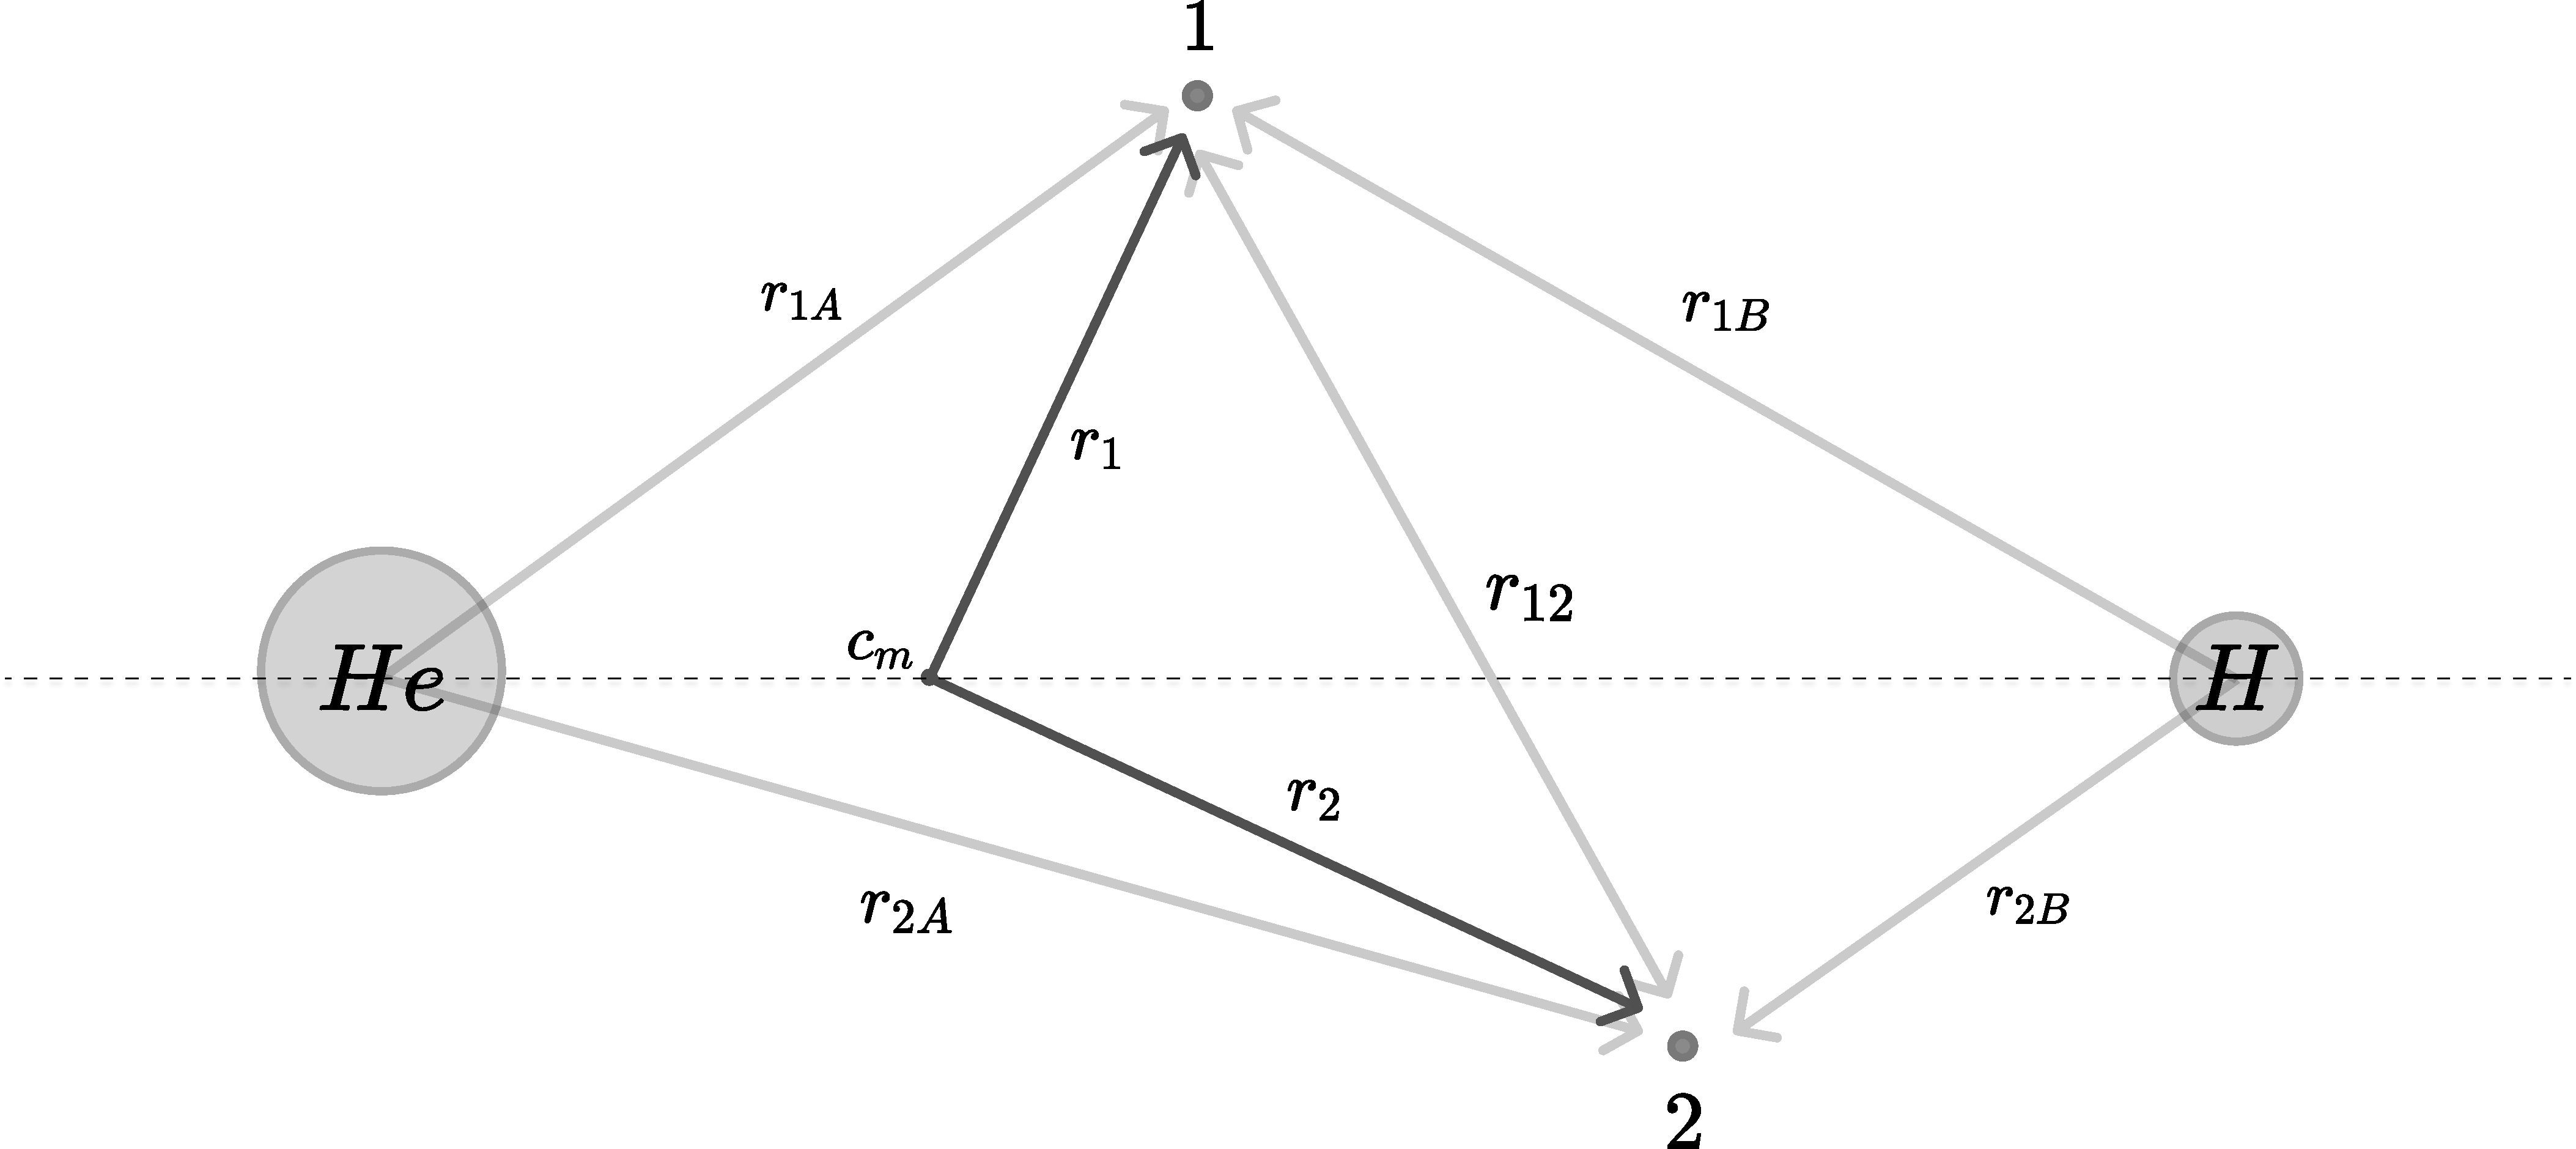
\includegraphics[width=0.8\textwidth]{heh+.pdf}
    \caption{Visual representation of the molecule }
    \label{hehp}
\end{figure}

The HeH\textsuperscript{+} molecule consists of two electrons and two nuclei:  helium 4 nucleus(alpha particle) with a charge of 2 and a mass of $7294.2995365$ a.u. and a hydrogen nucleus with a charge of 1 and mass of $1836.15267247$ a.u. \cite{SCHWARTZ}

\section{Calculated quantities}

This thesis will attempt to provide accurate values of ground state energy and the permanent dipole moment as dependent of $R_{AB}$ for the molecule in question. In case of HeH\textsuperscript{+} the ground state is a singlet state with $1{}^{1}\Sigma^{+}$ symmetry.

\section{Expected behavior of the system}
\label{expectations}

\subsection{Ground state energy}

As the distance between the nuclei grows the behavior oh the system should start to resemble the system comprised of two  completely independent nuclei. In such a degenerated system one should expect the two electrons to stay in proximity to the helium nucleus, as it has a greater charge than the helium nuclei. Therefore, the ground state energy of the system in question should asymptotically approach the energy of the ground state of the helium atom ($-2.903385831313$)\cite{SCHWARTZ} as $R_{AB}$ goes to $\infty$. As both of the nuclei have a positive charge one should expect the ground state energy of the system to approach $\infty$ as $R_{AB}$ goes to $0$

\subsection{Permanent moment}

The previously mentioned resemblance to the degenerated system allows one to also deduce the expected behavior of permanent moment for large values of $R_{AB}$. As previously discussed one should expect the electrons of the system to remain in proximity to the helium nuclei. The origin of the coordinate system is placed at the center of mass of the nuclei, so its distance from the helium nucleus increases linearly with $R_{AB}$. As the value of the permanent moment is directly dependent on the distance between the electrons and the center of the coordinate system one should expect the permanent moment to asymptotically approach a linear function as $R_{AB}$ goes to $\infty$ and for large R all electronic density is concentrated around helium

\chapter{Results}

\section{Final values and their uncertainties}

As $\Omega$ increases the subbasis it defines includes more functions from the full basis as given by \ref{KWdef}. This implies that the value of $\Omega$ has to be inversely proportional to the uncertainty of the calculated values and that these values become infinitely precise as $\Omega$ approaches $\infty$. It can be observed that for all values of $\Omega$ and $R_{AB}$ the functions with the lower cumulative values of $n$ are the ones contributing most into the final form of the wave functions. This fact will be further discussed later, but based on that observation one can expect that the differences between the deltas of the calculated values will get progressively smaller with $\Omega$ and approach 0 as $\Omega$ approaches $\infty$

\subsection{Energy}

\begin{figure}[H]
    \center
    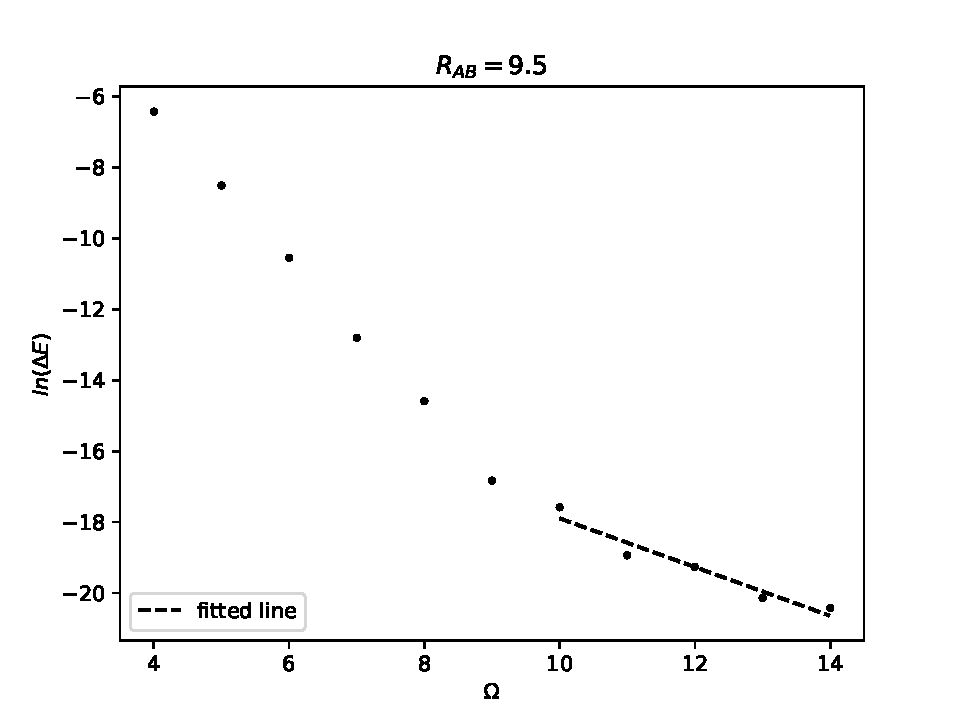
\includegraphics[width=0.8\textwidth]{E9.5.pdf}
    \caption{Graph of $ln\left(\Delta E\right)$ as dependent on $\Omega$ for  $R_{AB} = 9.5$}
    \label{delE fitted}
\end{figure}

When analyzing the behavior of the ground state energy differences between the neighboring values of omega decreases exponentially. As shown on the figure \ref{delE fitted} when examining the behavior of the natural logarithm of those differences can be approximated by the linear function. One can therefore evaluate the value of the ground state energy as it would be calculated for a full basis ($\Omega = \infty$) by fitting the linear function to the values mentioned previously, extrapolating the values of $\Delta E$ for $\Omega$ larger than the largest one used during calculations based on that fit and adding all of those differences to the value calculated for the largest $\Omega$. The value obtained in such a way will be treated as the actual value of the ground state energy, and the uncertainty will be calculated based on the variance of the fit parameters.

Note that for the data presented on graph \ref{delE fitted} the linear regression in not present when considering  $ln\left(\Delta E\right)$ for all the values of $\Omega$. This comes from the fact that the non-linear parameters for small omegas where better optimized, and therefore approach the exact value of the ground state energy more quickly. This was the case for all the non-linear parameters for all considered values of $R_{AB}$. In such case, fitting the linear function only to the last few data point allows one to avoid compromising the final calculated value of the ground state energy.

The dependence of $ln\left(\Delta E\right)$ on $\Omega$ was being represented by a linear function:

\begin{equation}
    y = ax+b
    \label{linear function}
\end{equation}

By fitting parameters $a$ and $b$ to the provided data points. $\Delta E$ was therefore given by

\begin{equation}
    \Delta E = e^{ax+b}
    \label{delEExp}
\end{equation}

Then, given the formula for the geometric series

\begin{equation}
    \sum_{k=s}^{k=\infty} r^k = \frac{r^s}{1-r}
\end{equation}

one can infer that the final value of energy will be given by 

\begin{equation}
    E_{\infty} = E_{\Omega_{mx}} + e^b\frac{e^{a\Omega_{mx}}}{1-e^{a}}
\end{equation}

Here $\Omega_{mx}$ represents the maximal value of $\Omega$ used in calculations. 
The variance of the energy was then obtained by repeating the previously described calculations for $a\pm \Delta a$ and $b\pm \Delta b$ ($\Delta \left(ab\right)$ represents the variance of the corresponding parameter) and finding the biggest possible difference from the previously calculated value obtainable in this way.

\subsection{Transitional moment}

For $ln\left(\Delta E\right)$ defined analogously as in the previous paragraph no apparent analytical behavior could be observed. Here the value of $d_{\Omega_{mx}}$ was considered as the exact value of $d$ and, considering the characteristic of obtained data described at the beginning of the chapter, the variance of that value was assumed to be the $\left|d_{\Omega_{mx}}-d_{\Omega_{mx}-1}\right|$

\section{Calculated values}

The calculations for all analyzed values of $R_{AB}$ where performed with the ionic basis because it proved to be satisfactory for this specific system. The final calculated values are presented in Table \ref{Results}

\subsection{Energy}

\begin{figure}[H]
    \center
    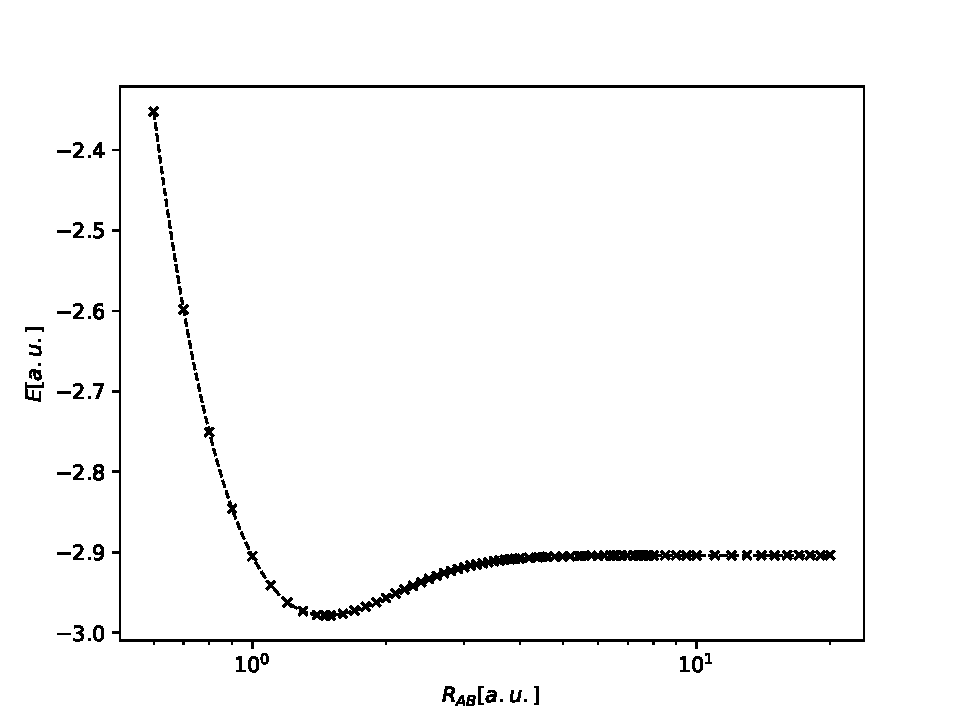
\includegraphics[width=0.99\textwidth]{14E.pdf}
    \caption{Graph of ground state energy as dependent on $R_{AB}$. Here $R_{AB}$ is presented in logarithmic scale. Crosses indicate numerical data}
    \label{E full}
\end{figure}

\begin{figure}[H]
    \center
    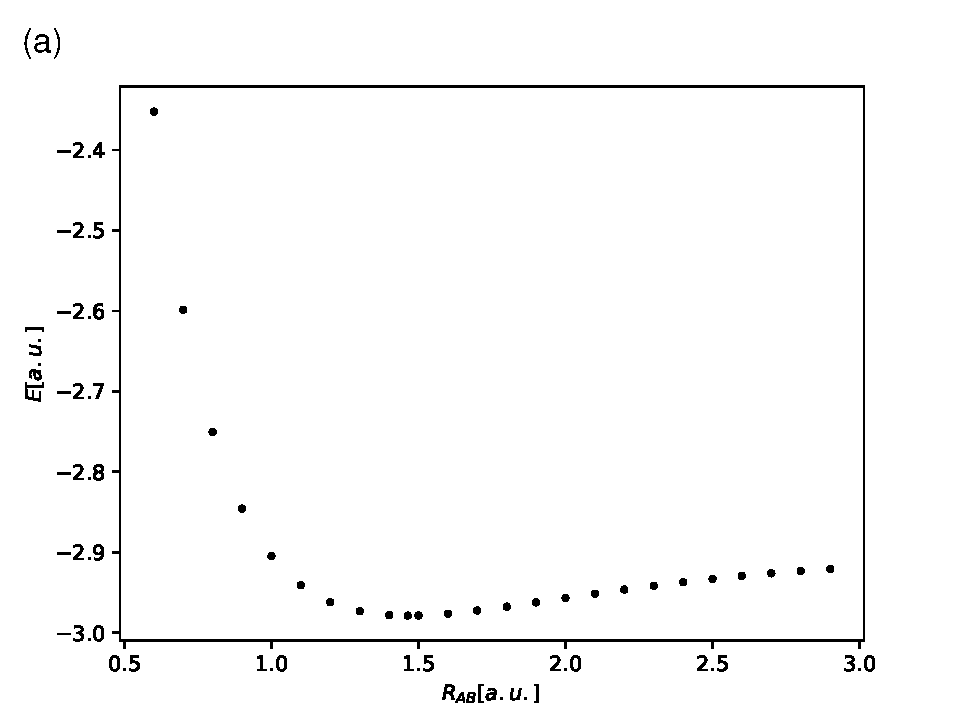
\includegraphics[width=0.49\textwidth]{14E_beginning.pdf}
    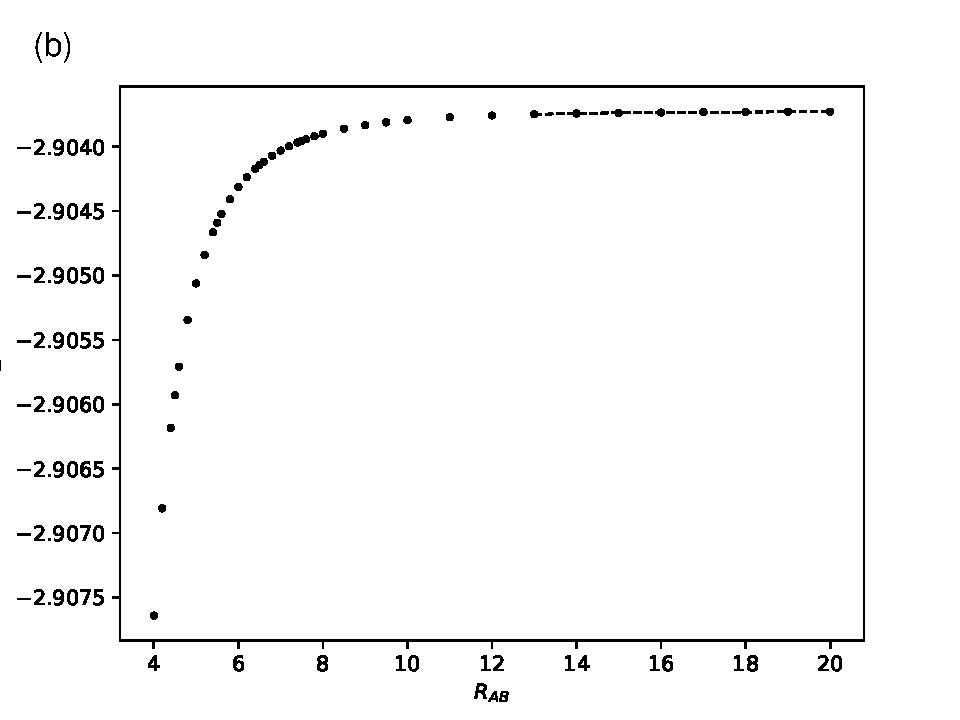
\includegraphics[width=0.49\textwidth]{14E_ending.pdf}
    
\includegraphics[width=0.49\textwidth]{empty.pdf}
    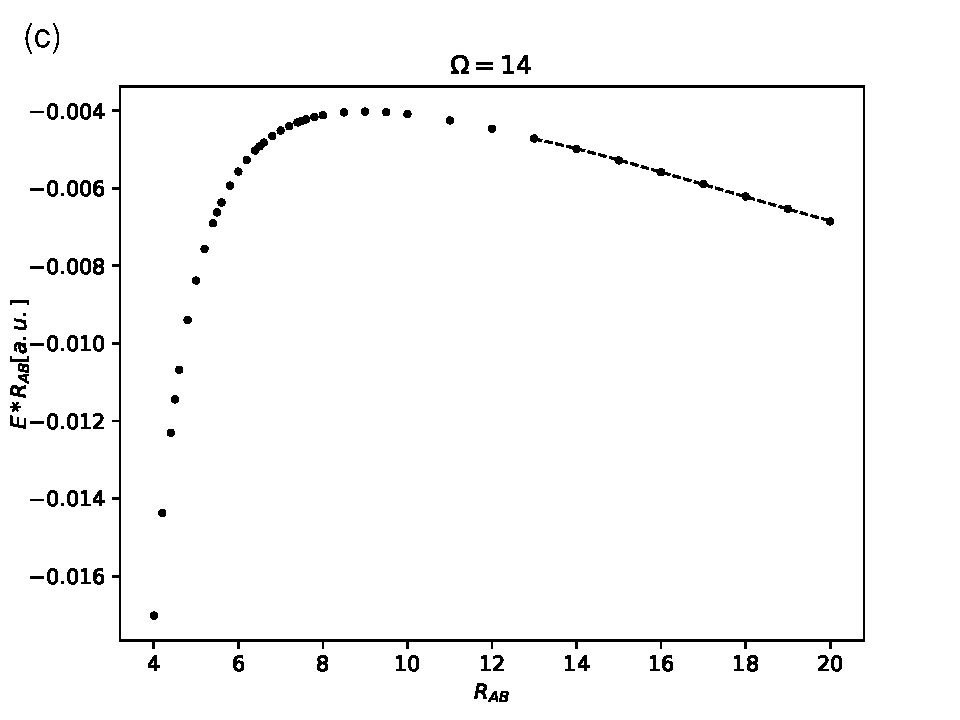
\includegraphics[width=0.49\textwidth]{14_ending_dos.pdf}
    \caption{Graphs of ground state energy as dependent on $R_{AB}$ calculated for $\Omega = 14$. Graph (a) shows the energy values for small $R_{AB}$. Graphs (b) and (c) energy values for large $R_{AB}$.}
    \label{E partial}
\end{figure}

The calculated values of ground sate energies seemed to approach $\infty$ as $R_{AB}$ approached $0$. For the examined values of $R_{AB}$ the energy was lowest for $R_{AB} = 1.463283$ reaching a value of $-2.978708310000(474)$. From that point as $R_{AB}$ grew the energy asymptotically approached a certain limit. The highest $R_{AB}$ considered was $R_{AB} = 20$, where the calculated energy was $-2.90372871900(1742)$. This behavior is consistent with expectations outlined in \ref{expectations}

\subsection*{Approximation for large $R_{AB}$}

As one should expect the ground state energy of the system to asymptotically approach the ground state energy of the helium atom $ E_{He}=-2.903385831313(3)$ as $R_{AB}$ goes to $\infty$ one can approximate the behavior of that value for large $R_{AB}$ with

\begin{align*} 
    E = E_{He} + \frac{a}{R_{AB}} + \frac{b}{{R_{AB}}^2} + \frac{c}{{R_{AB}}^3} + O\left({R_{AB}}^{-4}\right)\\
    \left(E - E_{He}\right){R_{AB}} = a + \frac{b}{{R_{AB}}} + \frac{c}{{R_{AB}}^2} + O\left({R_{AB}}^{-3}\right)\\\\
\end{align*}

Fitting $\left(a + \frac{b}{{R_{AB}}} + \frac{c}{{R_{AB}}^2}\right)$ to $\left(E - E_{He}\right)R_{AB}$ for $R_{AB} \geq 13$ returned a function

\begin{equation}
    \left(E - E_{He}\right)R_{AB} \approx -1.52(7) + \frac{0.272(9)}{{R_{AB}}} - \frac{0.0166(3)}{{R_{AB}}^2}
\end{equation}

The fitted function is presented on graph $(c)$ in \ref{E partial} Therefore for large values of $R_{AB}$ $ E\left({R_{AB}}\right)$ can be well approximated by

\begin{equation}
    E\left({R_{AB}}\right) \approx E_{He}- \frac{1.52(7)}{{R_{AB}}} + \frac{0.272(9)}{{R_{AB}}^2} - \frac{0.0166(3)}{{R_{AB}}^3}
\end{equation}

This approximation is plotted on graph $(b)$ in \ref{E partial}

\subsection{Transitional moment}

\begin{figure}[H]
    \center
    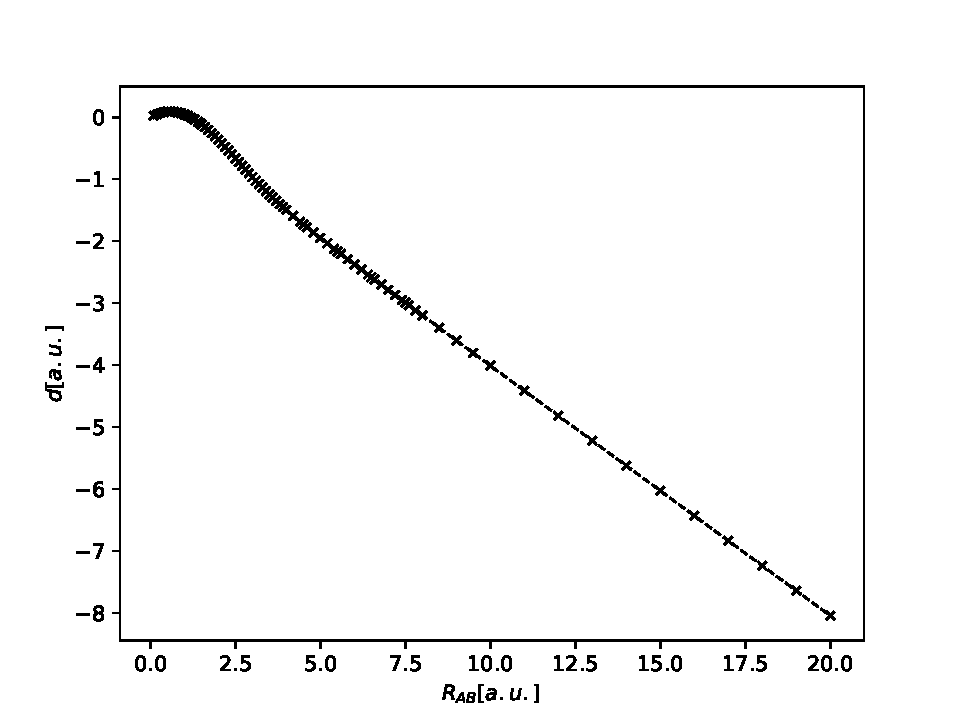
\includegraphics[width=0.99\textwidth]{14D.pdf}
    \caption{Graph of permanent moment as dependent on $R_{AB}$ calculated for $\Omega = 14$}
    \label{D full}
\end{figure}

\begin{figure}[H]
    \center
    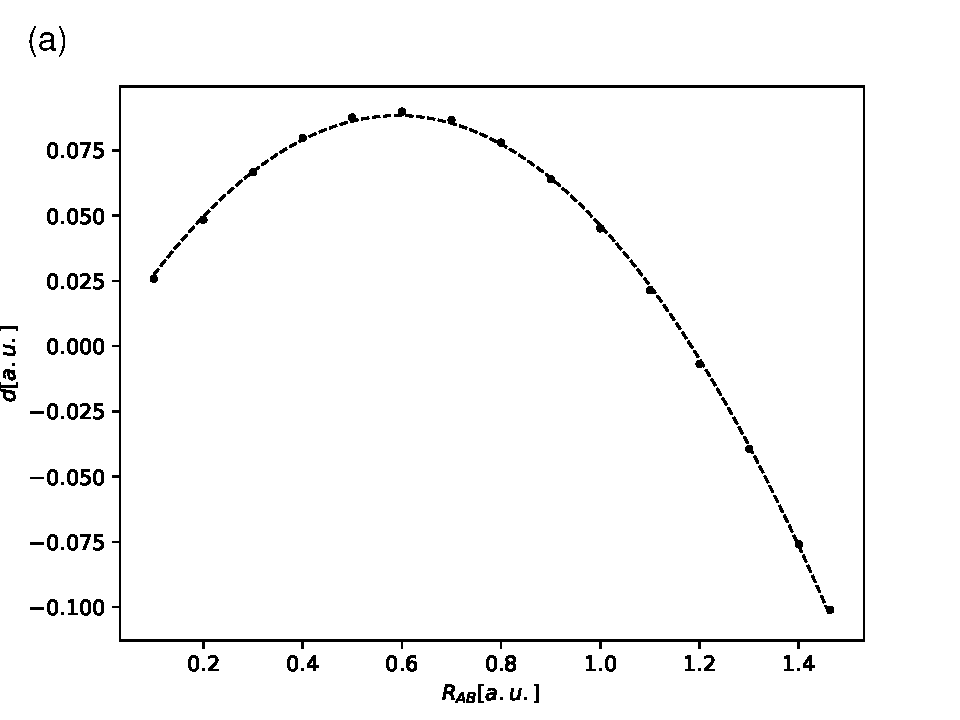
\includegraphics[width=0.49\textwidth]{14D_partial.pdf}
    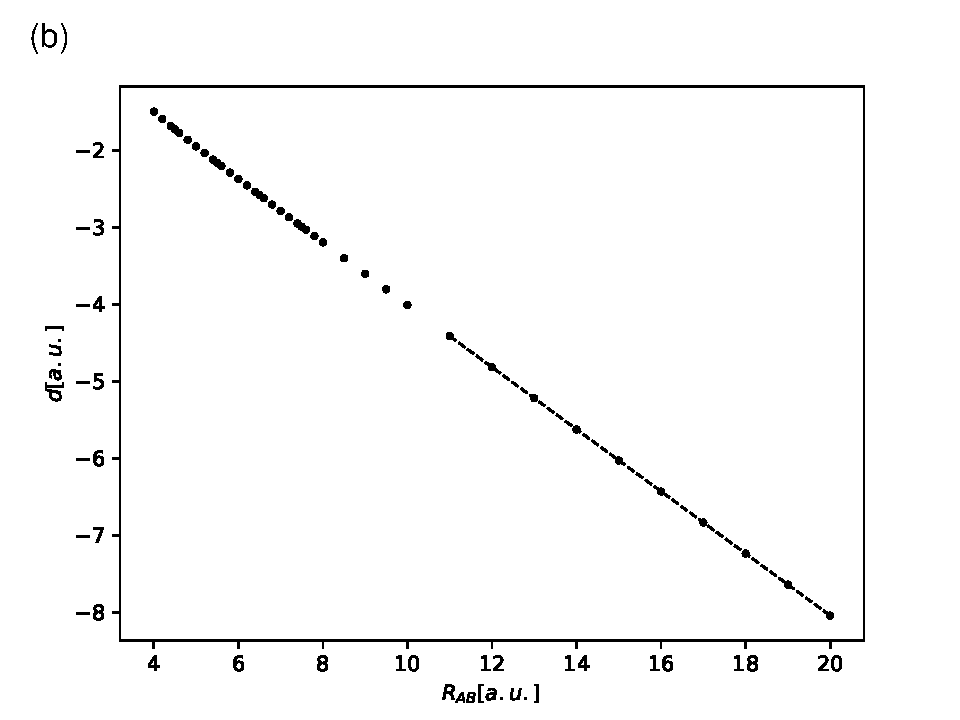
\includegraphics[width=0.49\textwidth]{14_partial2.pdf}
    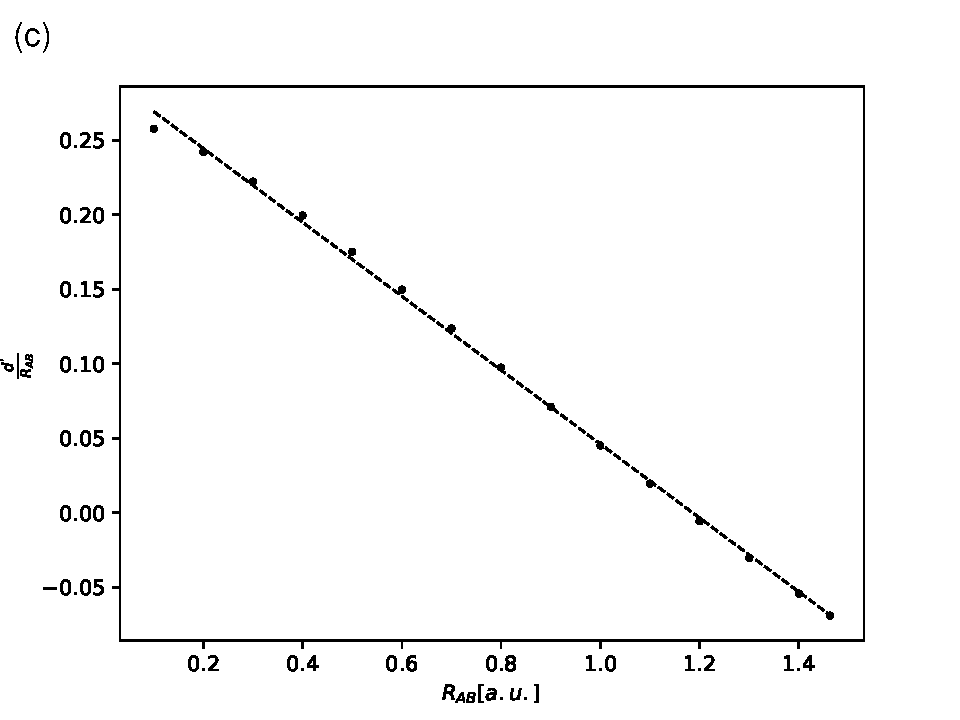
\includegraphics[width=0.49\textwidth]{14_partial_uno.pdf}
    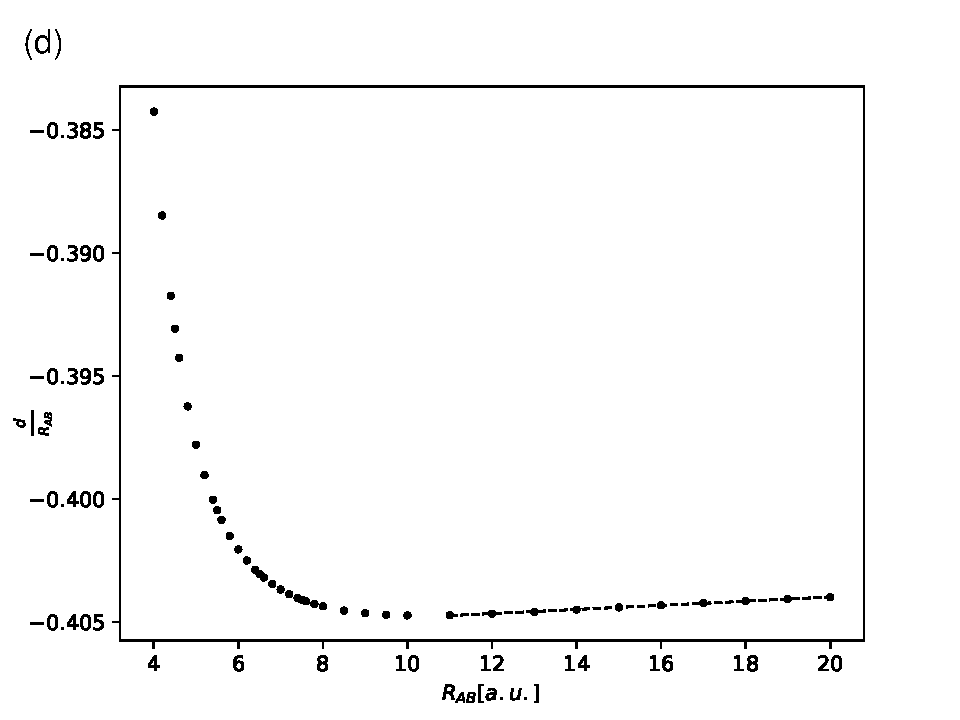
\includegraphics[width=0.49\textwidth]{14_partial2_uno.pdf}
    \caption{Graphs of the permanent moment as dependent on $R_{AB}$ calculated for $\Omega = 14$ with the fitted polynomials. $(a)$ shows the values of the permanent moment for small values of $R_{AB}$ with a fitted second order polynomial. $(b)$ shows the values of the permanent moment for large values of $R_{AB}$ with a fitted linear function. $(c)$ shows the dependency of the permanent moment as divided per $R_{AB}$ for small $R_{AB}$. $(d)$ shows the dependency of the permanent moment as divided per $R_{AB}$ for large $R_{AB}$. }
    \label{D partial}
\end{figure}

% [-0.25238788  0.29865978] [0.00137852 0.00163798]

The calculated values of ground sate energies seemed to approach $0$ as $R_{AB}$ approached $0$. For the examined values of $R_{AB}$ the moment was largest for $R_{AB} = 0.6$ reaching the value of $0.08986970428(12)$. From that point forward the $d$ decreased seemingly asymptotically to a certain linear function. The highest $R_{AB}$ considered was $R_{AB} = 20$, where the calculated moment was $-8.04062165500(38)$. This behavior is consistent with expectations outlined in \ref{expectations}

\subsection*{Approximation for small $R_{AB}$}

Knowing that $d\left(0\right) = 0$ one can approximate the behavior of $d$ for small values of $R_{AB}$ with

\begin{align*} 
    d = b {R_{AB}} + a {R_{AB}}^2  + O\left({R_{AB}}^{3}\right)\\
    \frac{d}{R_{AB}} = b  + a {R_{AB}} + O\left({R_{AB}}^{2}\right)
\end{align*}

Fitting $\left(b  + a {R_{AB}}\right)$ to $\frac{d}{R_{AB}}$ for $R_{AB} \leq 1.5$ returned a function
\begin{equation}
    \frac{d}{R_{AB}} \approx -0.253240(6)R_{AB}+0.30022(1)
\end{equation}

Therefore, $d\left({R_{AB}}\right)$ for small values of $R_{AB}$ can be approximated with

\begin{equation}
    d\left({R_{AB}}\right) \approx -0.253240(6)R_{AB}^2+0.30022(1)R_{AB}
    \label{smallD}
\end{equation}

These fits were plotted on graphs $(a)$ and $(c)$ in \ref{D partial}

\subsection*{Approximation for large $R_{AB}$}

When analyzing the behavior of $d$ for large values of $R_{AB}$ one can take advantage of the fact that as $R_{AB}$ approaches $\infty$ $d$ has to approach the permanent dipole moment of ionized hydrogen atom or "bare hydrogen nucleus" as measured with the origin of the coordinate system set at $hR_{AB}$ where $h$ is some constant. As for the symmetry of that system that value has to be equal to $0$ at $R_{AB} = 0$. Therefore, when analyzing the behavior of $d$ for large values of $R_{AB}$ one can perform a polynomial fit to $\frac{d}{R_{AB}}$ 

fitting a second order polynomial to $\frac{d}{R_{AB}}$ returned a function

\begin{equation}
    \frac{d}{R_{AB}}\approx 2.01956(3)*10^{-7}R_{AB}^2+7.7991(2)*10^{-5}R_{AB} + -0.4056194(1)
\end{equation}

This relationship is plotted on $(d)$ in \ref{D partial}

As previously mentioned we expect the transition moment to asymptotically approach a linear function as $R_{AB}$ goes to infinity. Therefore, one can deduce that for large $R_{AB}$ $(d)$ is well approximated by 

\begin{equation}
    d\approx -0.4056194(1)R_{AB}
\end{equation}

This approximation is plotted on graph $b$ in \ref{D partial}.

\chapter{Wave functions}

\section{Plots of the wave functions}

The final form of the symmetrized wave function is given by 

\begin{equation}
    \Psi = \sum_i c_i\left(1+P_{12}\right) \phi_i
    \label{wave function}
\end{equation}

Where $c$ represents the calculated parameters multiplying each of the basis functions, $\psi_i$ represents its corresponding function from the basis and $P_{12}$ represents the symmetry operator responsible for interchanging the electrons present in the system.

The square of the wave function represents the probability of measuring the position of the electron to be that specific spot in space. As the final symmetrized wave function is a function dependent six variables (every electron can potentially occupy any point in the three-dimensional space) it is difficult to visualize in its entirety in a convincing and understandable manner. Representing a specific cross-section of that function is however more realistic.

It can be observed that in the section between the nuclei on the line containing both of those nuclei the following relationships hold true

\begin{align*} 
    R_{AB} = R_{1A}+R_{1B}\\
    R_{AB} = R_{2A}+R_{2B}\\
    R_{12} = \left| R_{1A} - R_{2A} \right|
\end{align*}

Therefore, in that space the basis functions as described in\ref{KWdef} becomes

\begin{multline}
    \psi_{n_0 n_1 n_2 n_3 n_4}\left(r_{1A},r_{1B}\right) = e^{-y\left(r_{1A}-r_{1B}\right)-x\left(r_{2A}-r_{2B}\right)-\left(u+v\right)R_{AB}}\\
    {\left| R_{1A} - R_{2A} \right|}^{n_0}{\left(2 r_{1A}-R_{AB}\right)}^{n_1}{\left(2 r_{2A}-R_{AB}\right)}^{n_2}{R_{AB}}^{n_3+n_4}
    \label{degen}
\end{multline}

One can now see that on that specific section of space the basis functions degenerate to two variable functions. Those degenerated basis functions, and consequently the final wave function of the electrons, can easily be plotted.

\begin{figure}[H]
    \center
    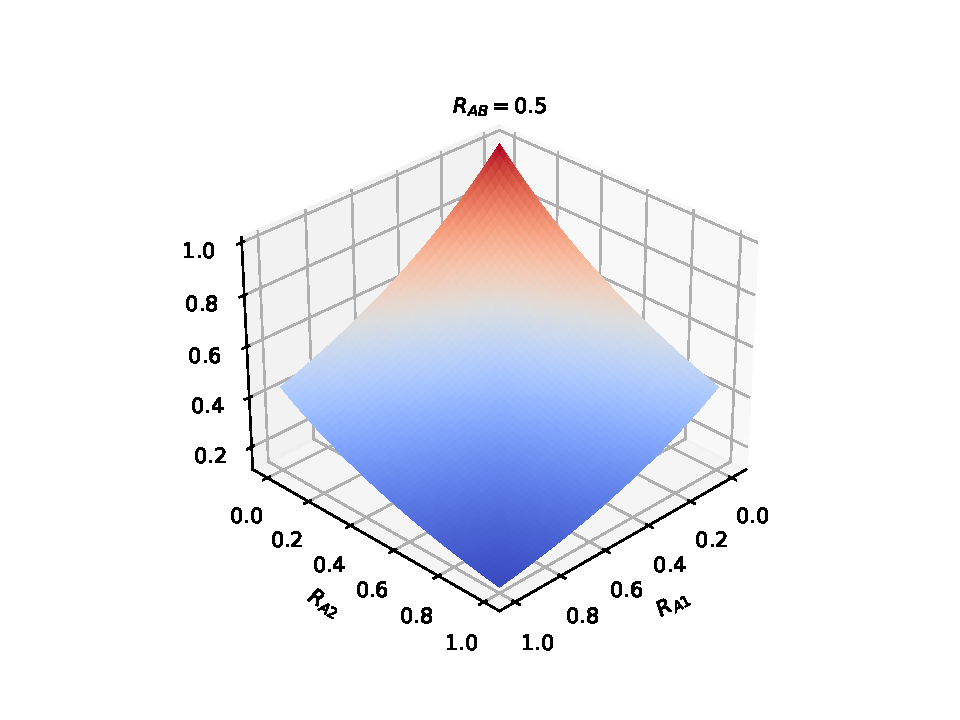
\includegraphics[width=0.49\textwidth]{0,5 (2).pdf}
    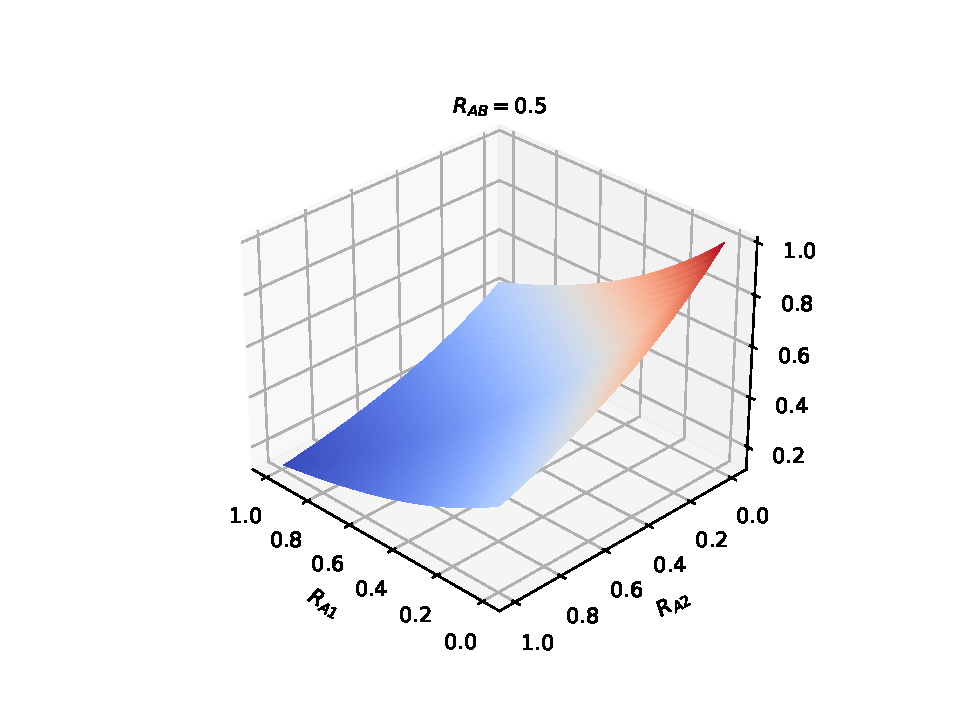
\includegraphics[width=0.49\textwidth]{0,5 (3).pdf}
    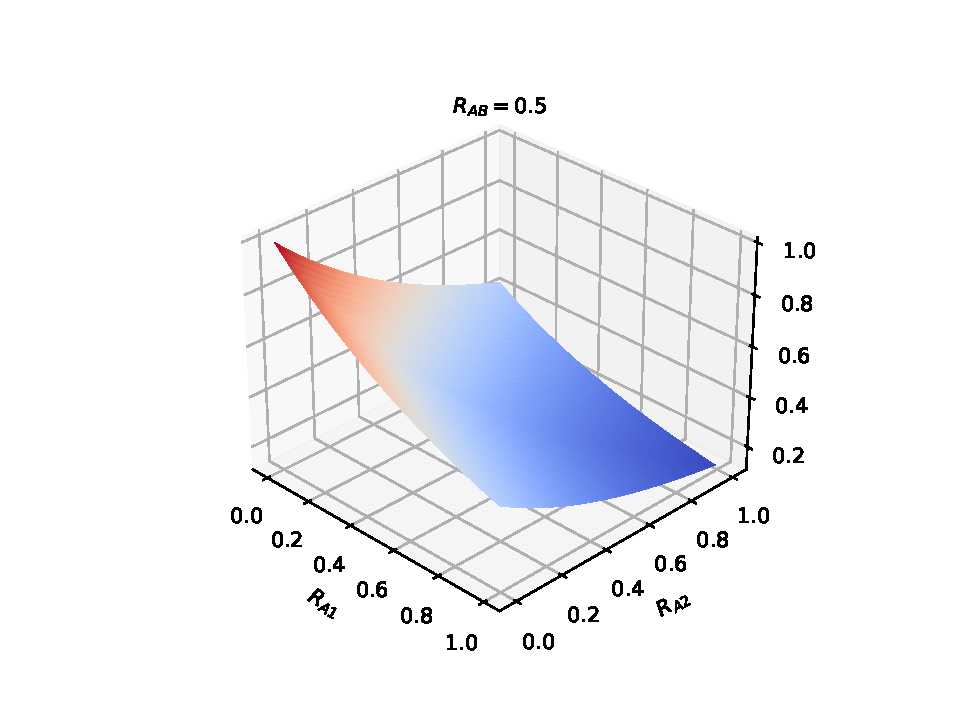
\includegraphics[width=0.49\textwidth]{0,5 (1).pdf}
    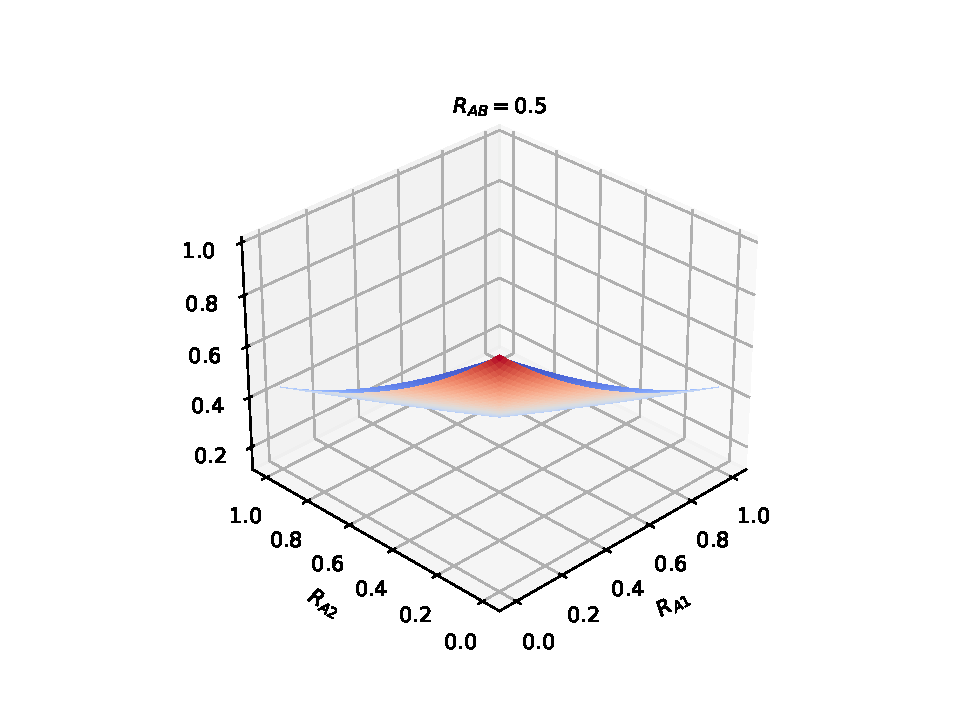
\includegraphics[width=0.49\textwidth]{0,5 (4).pdf}
    \caption{
        Auxiliary representation of the behavior of the squared value of the wave function in the section between the nuclei on the line containing both of those nuclei for $r_{AB} = 0.5$}
    \label{wave 0.5}
\end{figure}

\begin{figure}[H]
    \center
    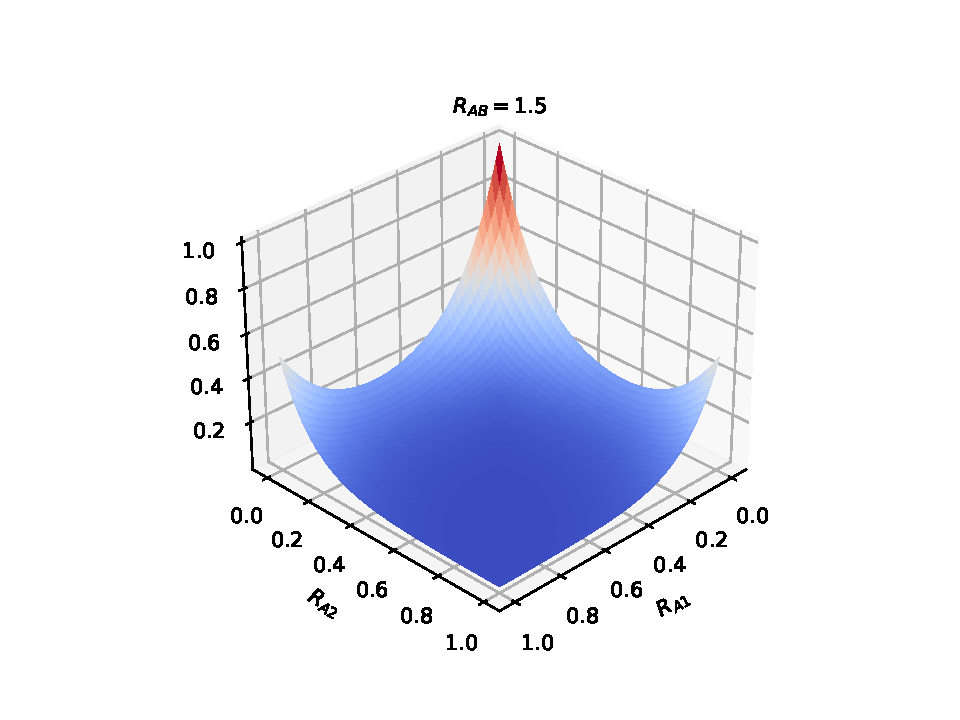
\includegraphics[width=0.49\textwidth]{1.5 (2).pdf}
    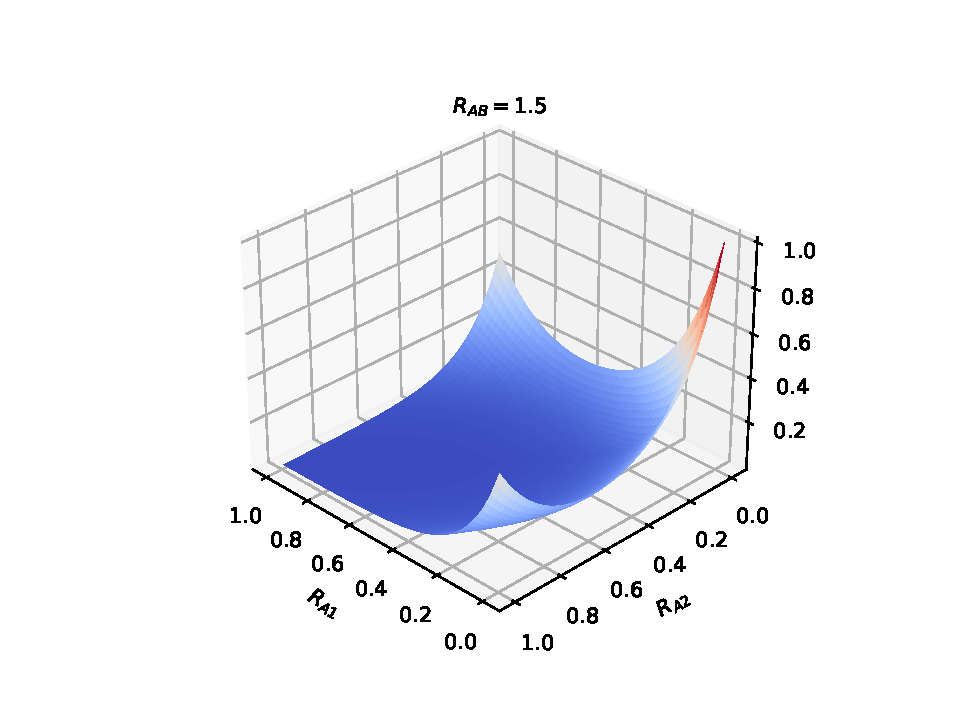
\includegraphics[width=0.49\textwidth]{1.5 (3).pdf}
    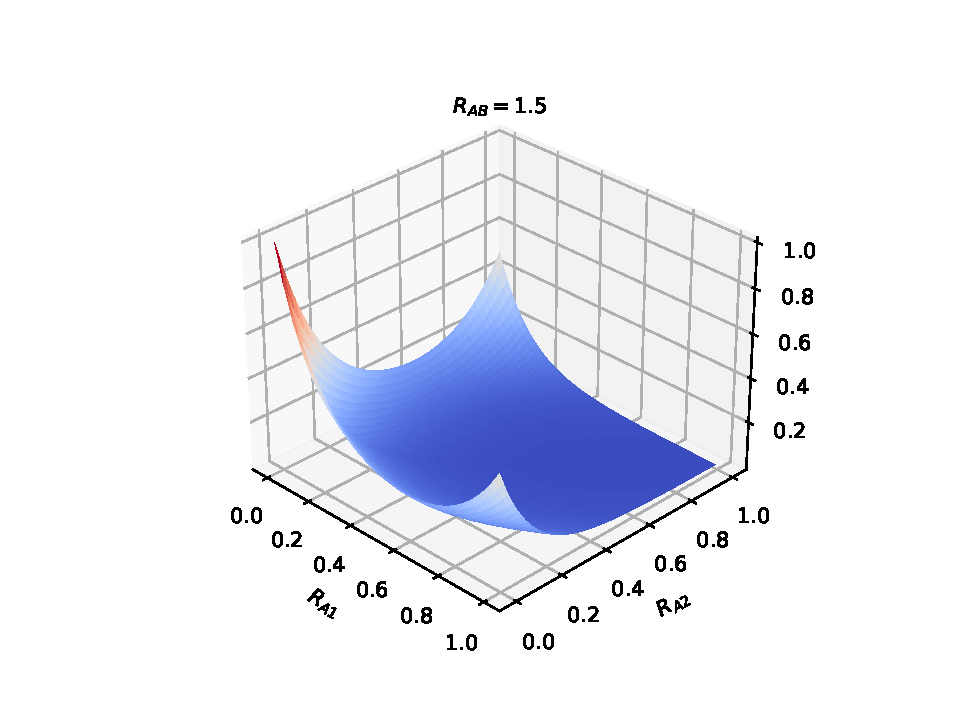
\includegraphics[width=0.49\textwidth]{1.5 (1).pdf}
    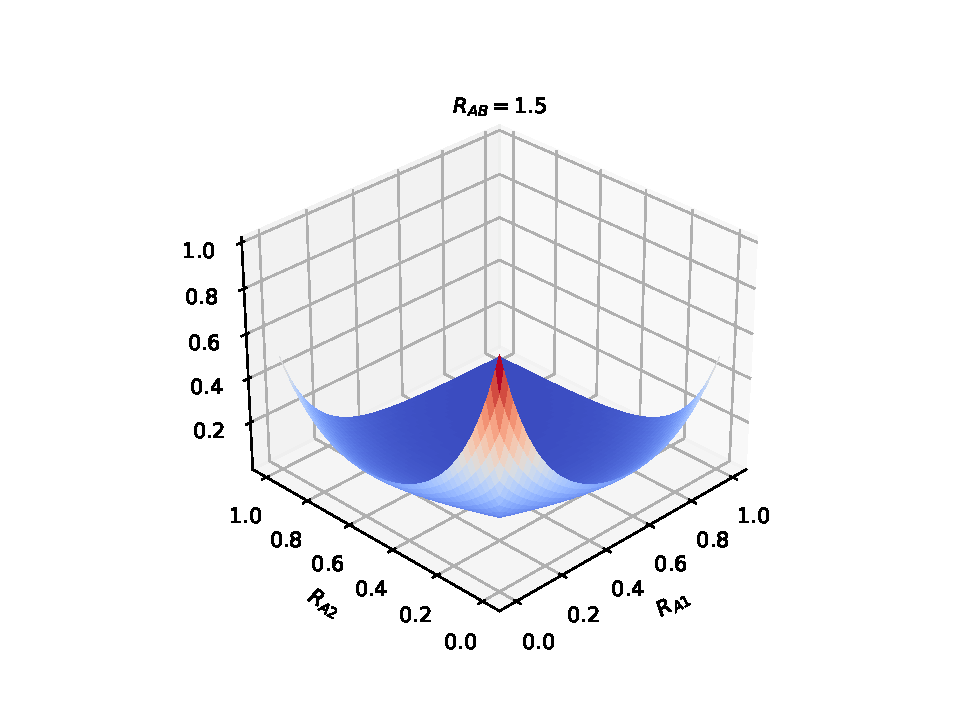
\includegraphics[width=0.49\textwidth]{1.5 (4).pdf}
    \caption{
        Auxiliary representation of the behavior of the squared value of the wave function in the section between the nuclei on the line containing both of those nuclei for $r_{AB} = 1.5$}
    \label{wave 1.5}
\end{figure}

\begin{figure}[H]
    \center
    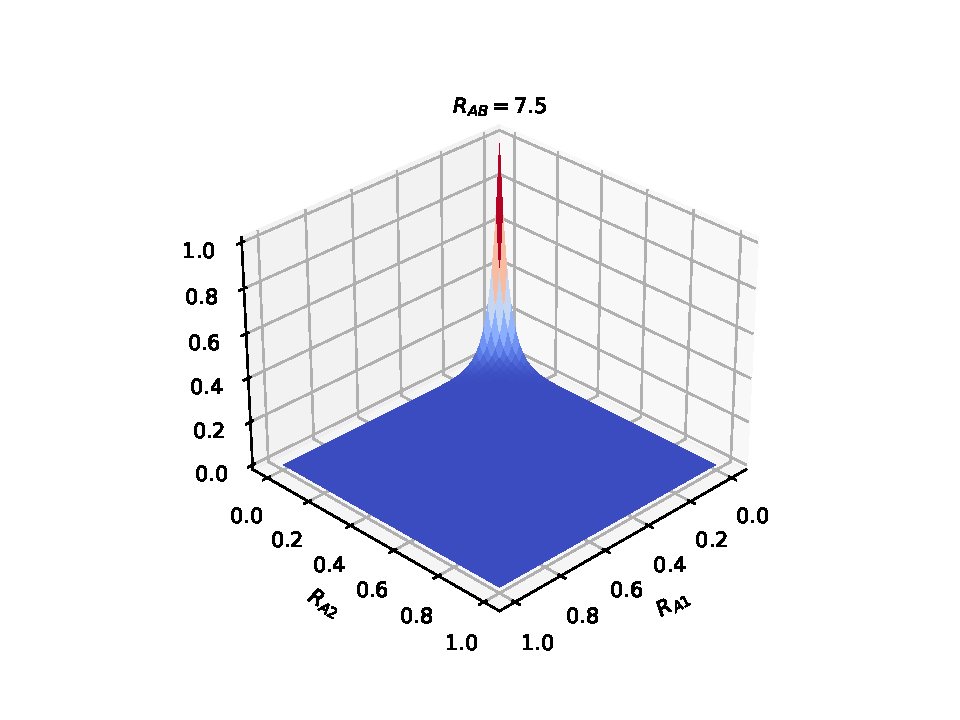
\includegraphics[width=0.99\textwidth]{7.5 (1).pdf}
    \caption{
        Auxiliary representation of the behavior of the squared value of the wave function in the section between the nuclei on the line containing both of those nuclei for $r_{AB} = 7.5$}
    \label{wave 7.5}
\end{figure}

\begin{figure}[H]
    \center
    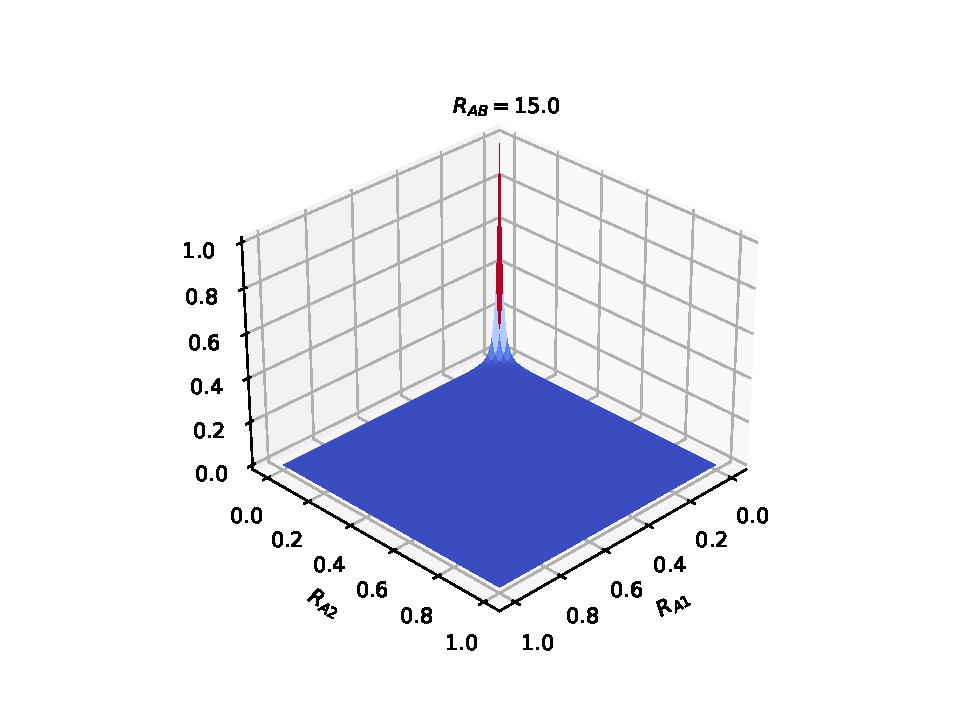
\includegraphics[width=0.99\textwidth]{15 (1).pdf}

    \caption{
        Auxiliary representation of the behavior of the squared value of the wave function in the section between the nuclei on the line containing both of those nuclei for $r_{AB} = 15$}
    \label{wave 15}
\end{figure}

Graphs \ref{wave 0.5}\ref{wave 1.5}\ref{wave 7.5}\ref{wave 15} present the plots of the final wave functions in the previously defined region for different values of $R_{AB}$. As these graphs don't represent the entire wave function at every point in space the units of the $z$ value where assumed to be arbitrary and have been normalized so that the maximal plotted value was $1$. $R_{2A}$ and $R_{1A}$ where scaled similarly. Here $0$ represents the position of the helium nucleus, whereas $1$ represents the position of the hydrogen nucleus. 
For small values of $R_{AB}$ measuring one of the electrons to be near the helium atom is relatively likely, but not as much as measuring the same electron to be near the helium atom. Measuring both electrons near the hydrogen nucleus is the least likely possibility of those presented. It can be observed that as $R_{AB}$ grows both of the electrons become more likely to concentrate around the helium nucleus. For $R_{AB} = 15$ measuring any of the electrons to be away from the helium atom is orders of magnitude less likely than measuring it to be close to the helium nuclei  This behavior is consistent with expectations presented in chapter \ref{expectations}. 

\section{Non-linear parameters}
The previously discussed degeneration of the two the one representing a helium atom can also be deduced from analyzing the optimized non-linear parameters. As mentioned in \ref{h2solv chapter} when parameters $u$ an $x$ in the ionic base are equal to one another the exponential part of the function depends solely on the distance of the electrons from the first nucleus (in this case helium). For $R_{AB}=20$ and $\Omega=14$ the optimized non-linear parameters are

\begin{align*} 
    x=1.246519767\\
    y=1.246519767\\
    u=1.253389667\\
    w=1.253389667\\
\end{align*}

So the basis function take the form of

\begin{multline}
    \psi_{n_0 n_1 n_2 n_3 n_4} \left( r_{1A}, r_{1B}, r_{2A}, r_{2B}, r_{12} \right) = e^{-2.49991\left(r_{1A}+r_{2A}\right)}e^{-0.0068699\left(r_{1B}+r_{2B}\right)}\\
    r_{12}^{n_0}{\left(r_{1A}-r_{1B}\right)}^{n_1}{\left(r_{2A}-r_{2B}\right)}^{n_2}{\left(r_{1A}+r_{1B}\right)}^{n_3}{\left(r_{2A}+r_{2B}\right)}^{n_4}
\end{multline}

Hence the input of the part dependent on the distance of the electrons form the hydrogen atom into the exponential part of the functions becomes negligible. For that reason the aforementioned basis is better suited for describing a single particle, allowing one to deduce these specific condition the system will likely be degenerated

For $R_{AB}=0.5$ and $\Omega=14$ the optimized non-linear parameters are

\begin{align*} 
    x=0.528981950\\
    y=0.528981950\\
    u=1.503050277\\
    w=1.503050277\\
\end{align*}

Here the basis function takes the form of 

\begin{multline}
    \psi_{n_0 n_1 n_2 n_3 n_4} \left( r_{1A}, r_{1B}, r_{2A}, r_{2B}, r_{12} \right) = e^{-2.03203\left(r_{1A}+r_{2A}\right)}e^{-0.974068\left(r_{1B}+r_{2B}\right)}\\
    r_{12}^{n_0}{\left(r_{1A}-r_{1B}\right)}^{n_1}{\left(r_{2A}-r_{2B}\right)}^{n_2}{\left(r_{1A}+r_{1B}\right)}^{n_3}{\left(r_{2A}+r_{2B}\right)}^{n_4}
\end{multline}

So the contribution of the hydrogen-dependent part of the exponential part of the function is more significant and therefore will have a not negligible input into the final form of the wave function    

\section{Discontinuity of the first derivative}

When inspecting the provided representations of the wave function a ridge along the line $R_{A1} = R_{A2}$ can be observed. This effect is present for all values of $R_{AB}$, and can be interpreted in a way that supports the notion that the obtained wave function forms are correct. Purely mathematically the effect originates from the term ${\left| R_{1A} - R_{2A} \right|}^{n_0}$ present in \ref{degen}. Here $R_{1A} - R_{2A}$ changes sign at the line described previously. In theoretical discussions the emergence of this effect can be explained by the Kato cusp condition that states that in a Coulomb potential the electron density has to have a cusp at the position of the particle\cite{Kato2011OnTE}. 
This property of the final wave function is a direct consequence of the explicitly correlated nature of the Kołos-Wolniewicz basis \ref{KWdef} and is one of the reasons why the basis is practical for describing two-electron systems


\chapter*{Summary}
\label{sec:summary}
\addcontentsline{toc}{chapter}{\nameref{sec:summary}}

The method discussed in the thesis provides a highly efficient way of calculating expected values of operators in two-electron diatomic particles The explicitly correlated nature of the Kołos-Wolniewicz basis it uses provides a good representation of the diatomic system, allowing the method to provide accurate results even if a relatively small subbasis is actually used during calculations. H2SOLV, a program implementing said method, allows one to obtain results with arbitrarily large precision. The ability to place constraints on the parameters defining the used subbasis makes the software versatile, allowing it to accurately calculate expected values of operators for a plethora of two atom particles. In some cases the extrapolating a value of the operator as calculated for a full basis can also be performed. The calculations of the permanent dipole moment and the ground state energy for the HeH\textsuperscript{+} performed using the program resulted in highly accurate(relative $10^{-10}$ precision) results that were consistent with expectations. The obtained wave functions were also behaved as theorized.

\newpage

% Please add the following required packages to your document preamble:
% \usepackage{longtable}
% Note: It may be necessary to compile the document several times to get a multi-page table to line up properly
% Final calculated values of permanent moment and energy with their uncertainties as extrapolated to complete basis set

\begin{longtable}[c]{lllll}
    \caption{Final calculated values of permanent moment and energy with their uncertainties as extrapolated to complete basis set}
    \label{Results}\\
    \hline
    \textbf{$R_{AB}[a.u.]$} & \textbf{$E[a.u.]$} & \textbf{$\Delta E \left(10^{10}\right)$} & \textbf{$d[a.u.]$} & \textbf{$\Delta d \left(10^{10}\right)$} \\ \hline
    \endfirsthead
    %
    \endhead
    %
    \hline
    \endfoot
    %
    \endlastfoot
    %
    0.1 & 12.8615512504  & 2.91   & 0.0257692303   & 1.14    \\
    0.2 & 3.1468614016   & 1.16   & 0.04845396304  & 0.76    \\
    0.3 & 0.1313796277   & 1.32   & 0.06667912778  & 0.49    \\
    0.4 & -1.2269260362  & 1.31   & 0.07982699005  & 0.31    \\
    0.5 & -1.94250013051 & 0.37   & 0.08759858282  & 0.65    \\
    0.6 & -2.3522984534  & 1.04   & 0.08986970428  & 0.12    \\
    0.7 & -2.5985865692  & 1.10   & 0.08663582018  & 0.01    \\
    0.8 & -2.7506630365  & 1.10   & 0.07798456023  & 0.16    \\
    0.9 & -2.8456470144  & 1.29   & 0.06407581492  & 0.33    \\
    1.0 & -2.90480442896 & 0.53   & 0.0451230635   & 5.38    \\
    1.1 & -2.9409376742  & 2.02   & 0.02137489205  & 0.76    \\
    1.2 & -2.9620474658  & 2.72   & -0.00690208042 & 0.99    \\
    1.3 & -2.9732784781  & 3.49   & -0.0394369962  & 1.29    \\
    1.4 & -2.9780118529  & 4.27   & -0.0759636387  & 1.67    \\
    1.463283                & -2.9787083100      & 4.74                                   & -0.1010236855      & 1.98                                   \\
    1.5 & -2.9785067356  & 5.00   & -0.1162236415  & 2.18    \\
    1.6 & -2.9762909893  & 5.62   & -0.1599643085  & 2.82    \\
    1.7 & -2.9724063622  & 6.12   & -0.2069322869  & 3.63    \\
    1.8 & -2.9675661261  & 6.50   & -0.2568649909  & 4.63    \\
    1.9 & -2.9622584850  & 6.75   & -0.3094819453  & 5.85    \\
    2.0 & -2.9568155526  & 6.91   & -0.3644781031  & 7.30    \\
    2.1 & -2.9514600380  & 8.97   & -0.4215207521  & 7.57    \\
    2.2 & -2.946337276   & 11.43  & -0.4802509544  & 7.69    \\
    2.3 & -2.941537505   & 14.30  & -0.5402896633  & 7.65    \\
    2.4 & -2.937111598   & 17.55  & -0.6012478751  & 7.41    \\
    2.5 & -2.933082339   & 21.14  & -0.6627395204  & 6.97    \\
    2.6 & -2.929452651   & 25.00  & -0.7243954049  & 6.32    \\
    2.7 & -2.926211683   & 29.04  & -0.7858764319  & 5.45    \\
    2.8 & -2.923339380   & 33.15  & -0.8468845762  & 4.38    \\
    2.9 & -2.920809917   & 37.22  & -0.9071705543  & 3.13    \\
    3.0 & -2.918594292   & 41.16  & -0.9665377189  & 1.71    \\
    3.1 & -2.916662255   & 44.87  & -1.0248422785  & 0.17    \\
    3.2 & -2.914983703   & 48.28  & -1.0819903799  & 1.47    \\
    3.3 & -2.913529665   & 51.33  & -1.1379328614  & 3.18    \\
    3.4 & -2.912272950   & 53.98  & -1.1926585660  & 4.91    \\
    3.5 & -2.911188534   & 56.19  & -1.2461870453  & 6.65    \\
    3.6 & -2.910253751   & 57.95  & -1.2985613303  & 8.36    \\
    3.7 & -2.909448335   & 59.27  & -1.349841256   & 10.02   \\
    3.8 & -2.908754357   & 60.13  & -1.400097632   & 11.62   \\
    3.9 & -2.908156102   & 60.57  & -1.449407404   & 13.13   \\
    4.0 & -2.907639892   & 60.60  & -1.497849803   & 14.55   \\
    4.2 & -2.906807934   & 73.96  & -1.592444183   & 23.26   \\
    4.4 & -2.906182473   & 87.02  & -1.684468942   & 32.58   \\
    4.5 & -2.905929164   & 93.18  & -1.729680940   & 37.47   \\
    4.6 & -2.905707946   & 98.97  & -1.774435440   & 42.52   \\
    4.8 & -2.90534411    & 109.07 & -1.862767353   & 53.06   \\
    5.0 & -2.90506192    & 116.82 & -1.949804964   & 64.19   \\
    5.2 & -2.90484047    & 140.09 & -2.035816214   & 81.15   \\
    5.4 & -2.90466461    & 163.70 & -2.12100959    & 100.41  \\
    5.5 & -2.90459021    & 156.29 & -2.16335152    & 103.82  \\
    5.6 & -2.90452335    & 186.24 & -2.20554637    & 122.11  \\
    5.8 & -2.90440864    & 206.38 & -2.28955114    & 146.32  \\
    6.0 & -2.90431455    & 223.02 & -2.37312039    & 172.96  \\
    6.2 & -2.90423665    & 288.54 & -2.45632924    & 223.69  \\
    6.4 & -2.90417159    & 346.86 & -2.53923663    & 285.42  \\
    6.5 & -2.90414305    & 404.91 & -2.58059224    & 358.21  \\
    6.6 & -2.90411683    & 389.33 & -2.62188919    & 359.53  \\
    6.8 & -2.90407041    & 415.49 & -2.70432425    & 446.76  \\
    7.0 & -2.90403081    & 430.10 & -2.78657197    & 546.60  \\
    7.2 & -2.90399683    & 406.45 & -2.86865702    & 757.95  \\
    7.4 & -2.90396751    & 338.17 & -2.9505998     & 1027.88 \\
    7.5 & -2.90395435    & 247.45 & -2.9915232     & 1420.73 \\
    7.6 & -2.90394209    & 279.29 & -3.0324172     & 1354.16 \\
    7.8 & -2.90391995    & 253.06 & -3.1141238     & 1651.97 \\
    8.0 & -2.90390058    & 19.12  & -3.19573149    & 782.32  \\
    8.5 & -2.90386179    & 225.86 & -3.3993839     & 1085.28 \\
    9.0 & -2.9038331657  & 7.04   & -3.60260910    & 293.74  \\
    9.5 & -2.903811670   & 46.69  & -3.80549946    & 218.29  \\
    10  & -2.9037952417  & 3.04   & -4.008122792   & 77.94   \\
    11  & -2.9037725364  & 2.25   & -4.412761466   & 19.21   \\
    12  & -2.9037582572  & 1.94   & -4.8168104630  & 4.44    \\
    13  & -2.9037489058  & 1.94   & -5.22044677667 & 0.94    \\
    14  & -2.9037425732  & 1.92   & -5.6237853227  & 2.31    \\
    15  & -2.9037381600  & 1.91   & -6.0269034856  & 2.77    \\
    16  & -2.903735016   & 17.71  & -6.4298549807  & 5.54    \\
    17  & -2.903732716   & 17.53  & -6.8326780637  & 4.91    \\
    18  & -2.903731006   & 17.44  & -7.2354005929  & 4.44    \\
    19  & -2.903729712   & 17.41  & -7.6380432503  & 4.08    \\
    20  & -2.903728719   & 17.42  & -8.0406216550  & 3.80    \\ \hline
\end{longtable}





\newpage
\bibliographystyle{unsrt}
\bibliography{ref}

\end{document}
"""



